%!TEX program=xelatex
%!TEX program=bibtex
%!TEX program=xelatex
%!TEX program=xelatex
% !Mode:: "TeX:UTF-8"
\documentclass[master,openany,twoside,a4paper,AutoFakeBold]{sudathesis}
\usepackage{tikz-dependency}
\usepackage{graphicx}
\usepackage{tikz}
\usepackage{tikz-qtree}
\usepackage{caption}
\usepackage{bbm}
\usepackage{letltxmacro}

\usepackage{pgfplots}
\usepackage{dashrule}
%\usepackage{colortbl}
%\usepackage{arydshln}
%\usepackage{multirow}
%\usepackage{multicol}
%\usepackage[SlantFont,BoldFont,CJKchecksingle,CJKnumber]{xeCJK}
%\setmainfont[BoldFont=SimHei ,ItalicFont=KaiTi_GB2312]{SimKai}
%\newcommand\fontnamekai{KaiTi_GB2312}

\usepackage{graphics}
\usepackage{pdfpages}

\newfontfamily\tgtermes{TeX Gyre Termes}
\makeatletter
  \begingroup
    \tgtermes
    \DeclareFontShape{\f@encoding}{\rmdefault}{m}{sc}{%
      <-> ssub * \f@family/m/sc}{}
    \DeclareFontShape{\f@encoding}{\rmdefault}{bx}{sc}{%
      <-> ssub * \f@family/bx/sc}{}
  \endgroup
\makeatother

\begin{document}

% 用户信息
% !Mode:: "TeX:UTF-8"

% 学院中英文名,中文不需要“学院”二字
% 院系英文名可从以下导航页面进入各个学院的主页查看
% http://www.buaa.edu.cn/xyykc/index.htm
\school
{计算机科学与技术学院}{School of XXX}

% 专业中英文名
\major
{计算机科学与技术~~~}{XXXX Engineering}

% 方向中英文名
\direct
{自然语言处理~~}{XXXX Engineering}

% 论文中英文标题
% Research on Chinese Named Entity Recognition With Noise Training Data
\thesistitle
{快速精准的句法分析方法研究}{Research on Fast and Accurate Syntactic Parsing Methods}

% 作者中英文名
\thesisauthor
{张宇~~~~}{Yu Zhang}

% 导师中英文名
\teacher
{李正华}{Zhenghua Li}


% 班级
\class{XXXX}

% 学号
\studentID{20184227035}

% 单位代码
\unicode{10285}

% 论文时间,用于首页
\thesisdate{2021}{3}

%\includepdf{content/mangshen-fengmian.pdf}

% 中英封面、提名页、授权书
\maketitle

% 正文前页码是大写罗马字母
\pagenumbering{Roman}
% 前言页眉页脚样式 % 摘要
\pagestyle{cnfrontmatter}
% !Mode:: "TeX:UTF-8"

% 中英文摘要
\begin{cabstract}
	句法分析任务是句子理解的重要中间过程之一.
	其中,概率估计一直是句法分析领域的一个核心问题.
	然而,无论是神经网络方法还是深度学习时代以前的方法,采用基于全局概率模型的句法分析工作都非常少,主要的原因在于树形条件随机场(TreeCRF)推断的高复杂度.
	在本文中,我们提出将TreeCRF应用到依存句法和成分句法这两个主要的句法分析任务.
	为了解决TreeCRF的低效问题,关键的想法是批次化树结构的推断算法,并且用基于自动求导的反向传播代替Outside算法.
	目前句法模型被不断简化,采用局部损失目标是当前句法分析方法的一个趋势,我们则进一步在一阶TreeCRF的基础上采用了高阶拓展.
	高阶TreeCRF进一步增加了算法复杂度,为此,我们还提出利用基于平均场变分推断的近似推断算法代替精确推断的TreeCRF方法,从而增加了解析效率.

	具体而言,本文的研究内容主要包含三个方面:
	\begin{enumerate}

		\item 基于TreeCRF的高阶依存句法分析方法

		      本文提出将TreeCRF方法应用到神经依存句法分析器当中,并进一步提出了一个二阶TreeCRF的扩展.
		      导致TreeCRF低效的主要瓶颈在于Inside-Outside算法,尤其是Outside算法的计算.
		      为了解决这个问题,一方面,我们提出对Inside算法进行批次化,从而利用GPU的并行计算能力来加速,将算法复杂度从$O(n^3)$降低到了$O(n^2)$.
		      另一方面,我们还提出将复杂的Outside算法用高效的反向传播代替,显著提升了效率,使得一阶和二阶模型的速度分别达到了500和400句每秒.
		      我们在13个语言的27个数据集上进行了详细实验,结果表明了TreeCRF和高阶建模的有效性.

		\item 基于TreeCRF的高阶成分句法分析方法

		      本文提出将高阶TreeCRF应用到成分句法分析中.
		      为了解决效率问题,我们应用了和依存模型中一致的批次化技术和反向传播来加速.
		      此外,我们提出一个简单的两阶段解析方法,和前人的一阶段解析相比结果相当,但是更加高效.
		      我们还参考了依存句法的模型架构和参数设置,提出用双仿射打分机制替换传统打分方法,发现在双向LSTM编码器中引入的诸如Dropout的策略改进可以极大提升解析的性能.
		      在中英文三个基准数据集上的实验结果表明,我们提出的模型结果显著超越了现有方法,并且一阶和二阶模型的速度分别达到了1,092和598句每秒.
		      我们的模型在使用BERT之后达到了现有最好的结果.

		\item 基于变分推断的高效句法分析方法

		      为了解决精确推断的TreeCRF方法高复杂度的问题,本文提出在依存句法和成分句法分析中引入基于平均场变分推断的近似方法.
		      相比于高阶TreeCRF方法,变分推断将算法在GPU上的复杂度从$O(n^2)$降低到了$O(n)$,大大提升了模型效率.
		      在中英文共五个数据集上的实验结果表明,我们的二阶变分推断方法在性能上显著超越了一阶模型,达到了和二阶TreeCRF模型可比较的水平,与此同时在依存句法和成分句法上的解析速度分别达到了1,126句每秒和905句每秒,大大超越了精确推断的二阶TreeCRF.
		      此外,使用BERT之后,我们的变分推断方法的结果达到或接近了现有的最佳结果.

	\end{enumerate}

	综上,我们在依存和成分句法这两种句法分析任务上提出应用TreeCRF以及一个二阶TreeCRF拓展,显著提升了句法分析器的性能.
	我们采用批次化以及反向传播等加速技术,解决了TreeCRF的效率问题.
	本文同样还探究了变分法等近似方法对解析效率的影响.
	我们发现变分法在保持高阶模型的性能的同时,大大加快了解析速度.

	\vskip 21bp
		{\heiti\zihao{-4} 关键词:}
	句法分析,
	依存句法分析,
	成分句法分析,
	树形条件随机场,
	变分推断

	\begin{flushright}
		作~~~~~~~~者:***

		指导老师:***

	\end{flushright}
\end{cabstract}




\pagestyle{enfrontmatter}
% !Mode:: "TeX:UTF-8"

\begin{eabstract}
	Syntactic parsing is one of the most important intermediate processes of sentence comprehension.
	However, in both deep learning (DL) and pre-DL eras, very few works have adopted global probabilistic models, mainly due to the high complexity of probabilistic inference algorithm for syntax trees.
	In this thesis, we propose to apply TreeCRF to dependency and constituency parsing.
	Compared with previous works, the advantage of TreeCRF is to obtain tree/subtree probabilities, which is more useful for downstream tasks.
	The main bottleneck leading to the inefficiency of TreeCRF lies in the Inside-Outside algorithm, especially the calculation of the Outside pass.
	To solve this, on the one hand, we propose to batchify the Inside algorithm, so as to utilize the parallel computing power of GPU to speed up.
	On the other hand, we also propose to replace the complex Outside algorithm with efficient back-propagation.
	In deep learning era, models are greatly simplified.
	It's a trend to adopt local loss (classification) for both dependency and constituency parsing.
	We propose a high-order extension based on the first-order TreeCRF.
	High order modeling further increases the time complexity.
	To this end, we also try to apply the approximate mean field variational inference algorithm as an alternative to exact inference of TreeCRF method, improving the parsing efficiency greatly.
	We conduct experiments on several benchmark datasets of dependency and constituency parsing, and find that exact inference of high-order TreeCRF brings significant improvement.
	The proposed variational inference method achieves or approaches the performance of high-order TreeCRF method, and greatly improves the parsing speed.
	
	Overall, the main research content of this thesis includes three aspects:
	
	\begin{enumerate}
		\item We propose a TreeCRF-based high-order method for dependency parsing.
		      This thesis proposes a second-order TreeCRF extension to Biaffine Parser that adopts a local training objective, and uses adjacent sibling subtrees as second-order features.
		      To integrate second-order subtree scores more effectively, inspired by biaffine scorer, we propose a novel triaffine structure for scoring.
		      Second-order TreeCRF method causes severe efficiency issues.
		      To overcome this, we propose to batchify the Inside algorithm and use the GPU parallel computing ability to reduce the time complexity from $O(n^3)$ to $O(n^2)$.
		      In addition, we replace the complex Outside algorithm with back-propagation based on auto-differentiation, which significantly improves the efficiency and speed up the model to 400 sentences/s.
		      We conduct extensive experiments on 27 datasets in 13 languages.
		      Results show that second-order models lead to better convergence performance, perform well on global metrics, and is especially useful for partially annotated data.
		\item We propose a TreeCRF-based high-order method for constituency parsing.
		      This thesis proposes to apply high-order TreeCRF to constituency parsing.
		      To solve the efficiency issue, we apply batchification techniques and back-propagation consistent with the dependency model to accelerate.
		      Moreover, we propose a simple two-stage parsing approach, which has comparable results with previous one-stage methods, but is more efficient.
		      We also refer to the model architecture and parameter settings of dependency models, and propose to replace the traditional scoring method with a biaffine scoring mechanism.
		      We find that the parsing performance can be largely improved via better encoder settings like Dropout configuration, leading to similar results with current state-of-the-art Transformer encoder.
		      Experimental results on three Chinese and English benchmark datasets show that our proposed models significantly surpass existing methods.
		      In terms of parsing speed, our first-order and second-order models can parse over 1,092/598 sentences/s.
		      After using BERT, our models achieve new state-of-the-art performance on all datasets.
		\item We propose an efficient syntactic parsing method based on variational inference.
		      In order to deal with the high complexity of the TreeCRF method for exact inference, this thesis proposes to introduce an approximate method based on mean field variational inference for dependency and constituency parsing.
		      Compared with high-order TreeCRF, variational inference reduces the time complexity on GPU from $O(n^2)$ to $O(n)$, improving the model efficiency greatly.
		      We design different factor graphs and corresponding variational inference updating algorithms for dependency and constituency parsing.
		      Experimental results on five Chinese and English datasets show that our second-order variational inference method significantly outperforms the first-order model, and achieves comparable results with second-order TreeCRF models.
		      Meanwhile, our models can parse over 1,126 and 905 sentences/s on dependency parsing and constituency parsing respectively, greatly surpassing the exact inference of second-order TreeCRF methods .
		      Moreover, after using BERT, our variational inference method achieves or approaches the performance of current state-of-the-art models.
	\end{enumerate}
	
	In summary, we propose an efficient second-order TreeCRF extension for both dependency and constituency parsing, achieving the current state-of-the-art performance.
	We also apply the variational method to syntactic parsing.
	We find it greatly improves the parsing speed while has a similar performance to exact high-order modeling.
	\vskip 21bp
	{\bf\zihao{-4} Key words: }
	Syntactic Parsing,
	Dependency Parsing,
	Constituency Parsing,
	TreeCRF,
	Variational Inference
\end{eabstract}

\begin{flushright}
	Written by ***
	
	Supervised by ***
\end{flushright}


% 目录不设置页眉和页码
\makeatletter
\let \asas \ps@plain
\let \ps@plain \ps@empty
\makeatother
\pagestyle{empty}

% 生成目录
\tableofcontents
\setcounter{secnumdepth}{4}

\makeatletter
\let \ps@plain \asas
\let\asas\relax
\makeatother
\clearpage  %目录3页以上,使用cleardoublepage

% 正文页码样式
\mainmatter
% 正文页眉页脚样式
\pagestyle{mainmatter}
% 正文页码是阿拉伯数字
\pagenumbering{arabic}

% % 正文


\chapter{绪论}
\label{cha:intro}

\section{研究背景和意义}

自然语言处理(Natural Language Processing, NLP)是目前人工智能方兴未艾的领域之一。
一个完整的自然语言处理句子分析流程主要分为三个部分:1)词法分析;2)句法分析;3)语义分析。
其中词法分析包含了词性标注(Part-of-Speech Tagging)、命名实体识别(Named Entity Recognition, NER)以及消歧(Disambiguation)等子任务,中文中由于词语之间没有天然边界,还需要额外进行中文分词。
句法分析的目的是以句法树的形式刻画句子结构,主要包含了依存句法(Dependency Parsing)和成分句法(Constituency Parsing)分析这两种范式。
语义分析则是为了理解句子的内含语义,包含语义角色标注(Semantic Role Labeling, SRL)、语义依存分析(Semantic Dependency Parsing, SDP)和抽象语义表示(Abstract Meaning Representation, AMR)等子任务。

上述的三个流程通常以管道的方式进行,而句法分析作为连接词法和语义分析的中间步骤,具备十分重要的研究价值。
目前存在着多种句法分析文法,例如组合范畴文法(Combinatorial Categorical Grammars, CCGs),成分文法(Constituency Grammars or Context Free Grammars, CFGs),以及依存文法(Dependency Grammars)。
其中依存文法对应的依存句法分析,和成分文法对应的成分句法分析是目前最常见的句法分析范式,也是本文主要的研究对象。

\begin{figure}[tb]
  \begin{center}
    \begin{dependency}%[arc edge, arc angle=80, text only label, label style={above}] %, hide label]
      %\begin{dependency} %[arc edge, arc angle=80] %, text only label, label style={above}] %, hide label]
      \begin{deptext}[column sep=.2cm] %[row sep=0.4cm, column sep=.22cm] %column sep=.2cm,
        \$$_0$ \& I$_1$ \& saw$_2$ \& Sarah$_3$ \& with$_4$ \&a$_5$ \& telescope$_6$ \\
        %\textsl{Gap:} \& $0.9$ \& $0.5$ \& $0.7$ \&[.4cm] $0.1$ \& $0.9$ \& $0.8$ \\
      \end{deptext}
      \depedge[edge style={black}]{3}{2}{nsubj}
      \depedge[edge style={black}]{3}{4}{dobj}
      \depedge[edge style={black}]{5}{7}{pobj}
      \depedge[edge style={black}]{7}{6}{det}
      \depedge[edge style={draw={rgb,255:red,76; green,114; blue,176}, thick}, label style={draw={rgb,255:red,76; green,114; blue,176}, text={rgb,255:red,76; green,114; blue,176}, semithick}]{1}{3}{root}
      \depedge[edge style={draw={rgb,255:red,76; green,114; blue,176}, thick}, label style={draw={rgb,255:red,76; green,114; blue,176}, text={rgb,255:red,76; green,114; blue,176}, semithick}]{3}{5}{prep}
    \end{dependency}
    \caption{
      一个完整依存树的例子.
      对于局部标注的场景,仅有一部分的弧被标注,例如图中两个粗蓝弧.
    }
    \label{fig:dep-tree-example} %
  \end{center}
\end{figure} %
依存句法分析的目的是识别句子中词语的修饰关系。
如图\ref{fig:dep-tree-example}所示,给定一个句子$\boldsymbol{x}=w_0,w_1,\cdots,w_n$,一棵依存树被定义为$\boldsymbol{t}=\{(i\rightarrow j,l)\mid 0\le i \le n,0 < j \le n,l \in \mathcal{L}\}$,其中$(i\rightarrow j,l)$是一条从头(head)$w_i$到修饰词(modifier)$w_j$的弧,弧的标签为$l \in \mathcal{L}$。
有标签树$\boldsymbol{t}$可以进一步被分解为$(\boldsymbol{y},\boldsymbol{l})$,即一棵无标签树$\boldsymbol{y}$和树上所有标签组成的序列$\boldsymbol{l}$。
得益于基准数据集宾州书库(Penn Treebank, PTB)的发布,以及深度学习技术的发展,目前依存句法分析技术得到了广泛研究。
其中计算自然语言学习会议(Conference on Computational Natural Language Learning, CoNLL)连续多年针对依存句法任务发布了评测任务,尤其是近年来依托通用依存(Universal Dependencies, UD) \citep{nivre-etal-2017-universal}项目发布的多语言评测比赛,大大推动了依存句法分析技术的进步。
由于结构简单、形式直观的特点,依存句法分析一直被广泛的应用在多个其他任务中,例如机器翻译 \citep{zhang-etal-2019-syntax}、关系抽取 \citep{song-etal-2019-leveraging}、意见挖掘 \citep{zhang-etal-2020-syntax}等等。

\begin{figure}[tb!]
	\centering
	\begin{subfigure}[b]{0.45\textwidth}
		\centering
		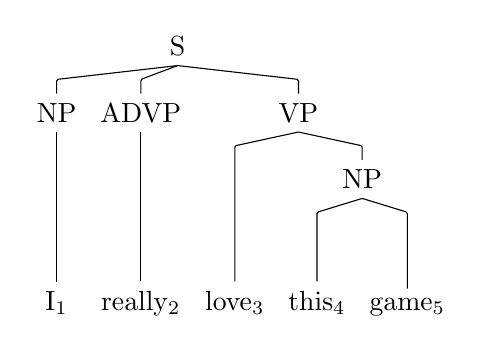
\begin{tikzpicture} [
				level distance=24pt,
				every tree node/.style={align=center,anchor=base},
				frontier/.style={distance from root=92pt},
				edge from parent/.style={draw,edge from parent path={(\tikzparentnode.south) {[rounded corners=0.5pt]-- ($(\tikzchildnode |- \tikzparentnode.south) + (0, -5pt)$) -- (\tikzchildnode)}}}
			]
			\Tree
			[.S
				[.NP I$_1$ ]
				[.ADVP really$_2$ ]
				[.VP love$_3$ [.NP this$_4$ game$_5$ ] ]
			];
		\end{tikzpicture}
		\caption{原始句法树}
		\label{fig:con-original-tree}
	\end{subfigure}
	\hfill
	\begin{subfigure}[b]{0.45\textwidth}
		\centering
		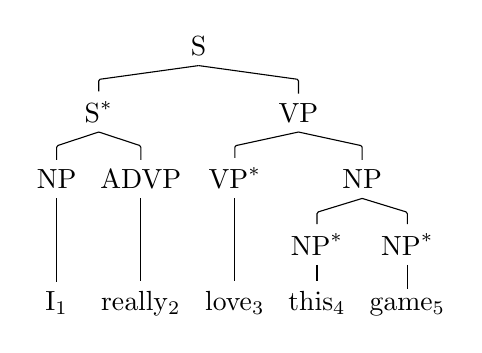
\begin{tikzpicture} [
				level distance=24pt,
				every tree node/.style={align=center,anchor=base},
				frontier/.style={distance from root=92pt},
				edge from parent/.style={draw,edge from parent path={(\tikzparentnode.south) {[rounded corners=0.5pt]-- ($(\tikzchildnode |- \tikzparentnode.south) + (0, -5pt)$) -- (\tikzchildnode)}}}
			]
			\Tree
			[.S
				[.$\textrm{S}^\ast$ [.NP I$_1$ ] [.ADVP really$_2$ ] ]
				[.VP
					[.$\textrm{VP}^\ast$ love$_3$ ]
					[.NP [.$\textrm{NP}^\ast$ this$_4$ ] [.$\textrm{NP}^\ast$ game$_5$ ] ]
				]
			];
		\end{tikzpicture}
		\caption{遵循乔姆斯基范式的左二叉化句法树}
		\label{fig:con-binaried-tree}
	\end{subfigure}
	\caption{
		成分句法树的例子.
		其中词性在这里被忽略
	}
	\label{fig:con-tree-full-figure}
\end{figure}

成分句法则旨在构建一个层次化的树结构。
如图\ref{fig:con-tree-full-figure},其中每个叶子结点是输入句子的每个词,而非终端结点作为区块(Constituents),如$\texttt{VP}_{3,5}$。
正式地,给定一个由$n$个词组成的句子$\boldsymbol{x}=w_1,\dots,w_{n}$,如图~\ref{fig:con-original-tree}所示,一棵成分句法树可以表示为$\boldsymbol{t}=\{((i, j),l)\mid 1\le i \le n,i \le j \le n,l \in \mathcal{L}\}$,其中$((i,j),l) \in \boldsymbol{t}$是一个包含$w_{i}...w_{j}$的区块,对应的句法标签为$l \in \mathcal{L}$。
本文中,为了方便模型处理,我们还将原始的树转换为了符合乔姆斯基范式(Chomsky Normal Form, CNF)的二叉树形式,如图~\ref{fig:con-binaried-tree}所示。
成分句法分析相比于依存句法而言,研究历史更加悠久,尽管目前没有依存句法技术那么流行,但是以其分析技术为基础衍生出了一系列在其他任务上的解析方法,例如UCCA语义分析 \citep{jiang-etal-2019-hlt}、嵌套命名实体识别 \citep{fu-etal-2021-nested}等等。

目前,针对句法分析任务,已经有大量的句法分析范式被提出,主要的有生成式方法、判别式方法,以及基于转移的方法、基于图的方法等等。
其中,基于图的方法尝试对每棵可能的句法树进行打分,然后选择一棵分值最高的树作为输出。
最简单的一阶方法将句法树分值分解为每个独立变量的分值之和,极大简化了模型建模。
与其他方法相比,基于图的方法无需设计复杂的转移系统,容易集成丰富的特征,可以达到很高的准确率,一直以来都是最流行的句法分析方法之一,因此也是本文所主要关注的句法分析方法。

传统的句法分析方法十分依赖于离散特征的人工设计和结构化建模。
由于缺乏对输入句子上下文的捕获能力,传统方法不得不手动设计诸如前缀、后缀、词性等特征,作为词输入的补充信息。
此外,显式的的树约束也是不可或缺的,模型依赖于Max Margin或TreeCRF等训练方法来全局最大化一棵树的分值/概率。

最近,由于深度神经网络的强大上下文编码能力,句法分析器的方法愈来愈有简单化的趋势。
作为依存句法和成分句法领域各自最有代表性的模型,\citet{dozat-etal-2017-biaffine}的依存句法分析器Biaffine Parser 和\citet{stern-etal-2017-minimal}的成分句法分析器正是符合这样的潮流。
其中Biaffine Parser: 1)采用了一个诸如双向LSTM或Transformer \citep{vaswani-2017-attention}这样强大的编码器;2)采取了简单的头选择训练损失函数。
类似地,\citet{stern-etal-2017-minimal}在双向LSTM编码器的基础上采取了Max Margin训练目标最大化正确树的分值,而\citet{gaddy-etal-2018-whats}更进一步,直接采取二分类方法判断短语树的每个组块是否存在。
这些方法由于建模简单,速度很快,因此一直是当前最为流行的句法分析方法。

有鉴于此,我们尝试在本文中将传统方法与现代的句法分析器做一个连接。
首先,我们在章节~\ref{cha:dep-crf}和章节~\ref{cha:con-crf}中采用了TreeCRF代替了当前流行的局部训练损失目标或者Max Margin方法。
与这些方法相比,TreeCRF的主要优势在于可以获得树/子树概率。
不同于没有上下界的分值,树/子树概率是评估解析置信度的更好指标,此外也可以作为一种软特征方便地作为下游任务的输入 \citep{zhang-etal-2019-syntax,zhang-etal-2020-syntax}。
主要限制TreeCRF应用的原因在于Inside-Outside算法的高复杂度问题,尤其是Outside过程,一般两倍慢于Inside。
对此,我们主要从两个方面尝试解决:
1)我们为Inside算法设计了精巧的批次化方法,使得TreeCRF能够利用GPU的并行计算能力大大加速;
2)得益于集成了自动求导机制的深度学习库的出现,我们无需和前人一样需要在CPU上进行完整的Inside-Outside过程得到梯度,而是将Outside过程由高效的反向传播机制代替。

此外,已经有很多工作证明,在模型中引入包含更多变量交互的高阶特征可以极大提升句法分析的准确率 \citep{mcdonald-pereira-2006-online,chen-manning-2014-fast,ji-etal-2019-graph}。
因此在章节~\ref{cha:dep-crf}和章节~\ref{cha:con-crf}中,我们在一阶模型的基础上引入了一个高阶TreeCRF的拓展。
为了能够对二阶子树特征打分,我们还参考Biaffine打分器为其设计了一个Triaffine机制。
结果表明,高阶TreeCRF在大多数数据集上都带来了显著的提升。

尽管可以应用批次化技术,高阶TreeCRF仍不可避免地加剧了推断算法效率低下的问题。
在机器学习社区中,研究者在针对推断算法高复杂度或者不可精确推断问题时,一个通常的做法是尝试采用近似推断算法。
因此在章节~\ref{cha:vi}中,我们还尝试了利用近似的平均场变分推断(Mean Field Variational Inference, MFVI)方法来代替高阶TreeCRF。
和其他同样在句法分析中广泛应用的近似推断算法,例如循环置信传播 \citep{smith-eisner-2008-dependency}和对偶分解 \citep{martins-etal-2009-concise},相比,MFVI的效率更高,收敛更快,并且通常可以达到更好的结果 \citep{wang-etal-2019-second}。
此外,MFVI能够方便的得到树/子树的概率,这保留了TreeCRF的优势。
我们在依存句法和成分句法分析两种范式中分别设计了两种不同的因子图以及变分推断迭代算法,结构表明MFVI在达到和高阶TreeCRF相接近的性能的同时,显著提升了句法模型的解析速度。

\section{数据集和评价指标}

\begin{table}[tb!]
    \centering
    \caption{依存句法分析数据集的数据统计,包含句子数和标签数.}
    \begin{tabular}{lrrr|c}
        \toprule
                & \#Train & \#Dev & \#Test & \#labels \\[1pt]
        \midrule
        % \\[-8pt]
        PTB     & 39,832  & 1,700 & 2,416  & 45       \\
        CoNLL09 & 22,071  & 1,762 & 2,556  & 41       \\
        NLPCC19 & 29,991  & 4,098 & 8,295  & 22       \\
        \bottomrule
    \end{tabular}
    \label{table:dep-statistics}
\end{table}

\noindent\textbf{数据.}
对于依存句法分析,我们在13个语言的27个数据集上进行了实验和分析,包含两个广泛使用的数据集:英语的斯坦福依存规范 \citep{chen-manning-2014-fast}的宾州树库(Penn Treebank, PTB)和中文的CoNLL09数据 \citep{hajic-etal-2009-conll}。
我们还采用了公开于NLPCC19跨领域句法分析任务的中文数据集 \citep{peng-etal-2019-overview},其中一共包含了四个源领域和三个目标领域。
方便起见,我们直接合并了四个领域的Train/Dev/Test数据到更大的数据集。
这些数据的一个特征是大部分句子都是利用基于主动学习的局部标注得到的。
表~\ref{table:dep-statistics}列出了相关数据的统计信息。
最后,遵循 \citet{ji-etal-2019-graph}和 \citet{zhang-etal-2019-empirical},我们在Universal Dependencies (UD) v2.2和v2.3上进行了实验。
我们采用了\citet{zeman-etal-2018-conll}使用的300维多语言预训练词向量,并采用CharLSTM表示作为输入。
对于UD2.2,为了和\citet{ji-etal-2019-graph}公平比较,我们和CoNLL18任务一样 \citep{zeman-etal-2018-conll},使用了毛文本,并且直接使用了他们的句子分割和符号化的结果。
对于UD2.3,为了与\citet{zhang-etal-2019-empirical}比较,我们报告的结果使用了正确词性。

对于成分句法分析,我们主要在三个中文和英文的数据集上进行实验。
前两个数据集,即PTB和CTB5.1,是句法分析社区中比较常用的两个数据集。
我们遵循了传统的Train/Dev/Test数据分割。
考虑到CTB5.1的Dev/Test都只有大约350句,为了得到更加稳定一致的结果,我们还在更大的CTB7数据上进行了实验,相关的数据分割设置参考了官方手册建议。
表~\ref{table:con-statistics}列出了相关数据的统计信息,其中UD的数据较多,因此不一一列举。
可以看到CNF转换引入了很多新的区块标签,其中大部分(大约75\%)都源于连续单链的折叠过程。

\begin{table}[tb!]
    \centering
    \caption{成分句法分析数据集的数据统计,包含句子数和标签数.
        对于``\#labels'',我们列出了原始树和CNF树对应的标签数.}
    \begin{tabular}{lrrr|cc}
        \toprule
               & \multirow{2}{*}{\#Train} & \multirow{2}{*}{\#Dev} & \multirow{2}{*}{\#Test} & \multicolumn{2}{c}{\#labels}       \\
               &                          &                        &                         & original                     & CNF \\[1pt]
        \midrule
        % \\[-8pt]
        PTB    & 39,832                   & 1,700                  & 2,416                   & 26                           & 138 \\
        CTB5.1 & 18,104                   & 352                    & 348                     & 26                           & 162 \\
        CTB7   & 46,572                   & 2,079                  & 2,796                   & 28                           & 265 \\
        \bottomrule
    \end{tabular}
    \label{table:con-statistics}
\end{table}

\noindent\textbf{评价指标.}
对于依存句法分析,我们使用无标签/有标签附着分值(Unlabeled/Labeled Attachment Score, UAS/LAS)作为主要的评价指标,其中UAS指头正确的词数占总词数之比,LAS则进一步还要求词的头正确的同时弧上的标签也正确。
评价时,PTB中的词性会被忽略掉。
对于局部标注的NLPCC19数据,我们采用了官方的评价脚本,直接忽略了没有正确头标注的词。
我们采用了Dan Bikel的随机解析评价比较器来进行显著性检验。

对于成分句法分析,在解析之后,我们将最佳的CNF树转化为\textit{n}-ary树再进行评价。
这里有必要提及一些有用的细节。
由于解码算法没有相应的约束,预测的最佳CNF树可能包含很多不合法的产生式。
以图~\ref{fig:con-binaried-tree}为例,模型可能输出$\texttt{VP}_{3,5} \rightarrow \texttt{PP}^{\ast}_{3,3} ~ \texttt{NP}_{4,5}$,其中 $\texttt{VP}$和$\texttt{PP}^{\ast}$是不兼容的。
在\textit{n}-ary后处理过程中,我们直接忽略了``$\mathtt{\ast}$''符号之前具体的字符串$\texttt{PP}$。
有鉴于此,如果解码的时候增加一定的约束,结果有可能进一步提高,这里我们留待作为后续的工作。
我们使用了标准的区块级别的准确率、召回率和$\mathrm{F}_1$值($\mathrm{P}$/$\mathrm{R}$/$\mathrm{F}_1$)作为评价指标,并使用\texttt{EVALB}工具\footnote{\url{https://nlp.cs.nyu.edu/evalb}}来评价。
特别地,一个例如$\texttt{VP}_{3,5}$的预测区块如果出现在了正确树中,那就被认为是正确的.\footnote{
	由于一些研究者可能会实现他们自己的评价脚本,为了比较的公平,需要澄清一些细节:
	1)一些诸如\texttt{\{-NONE-\}}的空区块在预处理的时候被移除了;
	2)评价的时候作为根结点的区块(英语里是\texttt{\{TOP,S1\}},中文里是空字符串) 被忽略了;
	3)包含一些例如\texttt{\{:,``,'',.,?,!\}}这些标点的区块也被忽略了;
	请注意中文标点会作为正常的字符被评价;
	4)一些在同一集合中的标签,例如\texttt{\{ADVP,PRT\}},被认为是等价的.}

\section{相关工作}
\label{sec:relworks}

\subsection{依存句法分析}

目前依存句法分析的两种主流方法分别是基于图的方法和基于转移的方法。
\textbf{基于图的方法}旨在从一个有向完全图中找到一棵概率(分值)最大的树,\textbf{基于转移的方法}将句法树的构建转化为一个移进和归约的动作序列,并寻求得到最优序列。

\citet{mcdonald-etal-2005-online}首先提出了基于图的训练方法。
他们提出采用基于动态规划的Eisner算法从有向完全图中得到分值最大的投影树,然后用Max Margin方法来训练。
后来\citet{mcdonald-etal-2005-non}将方法拓展到了非投影树解析领域,使用了ChuLiu/Edmods算法 \citep{chu-1965-shortest}得到分值最高的树。
由于学习和解码算法的复杂度很高,基于图的方法在给树打分时需要很强的独立性假设,其中最简单的弧分解假设认为树的每条弧相互独立(称为一阶模型),相应的树分值为所有弧的分值之和。
后来有研究者提出放宽独立性假设,将邻接兄弟、祖父、共同父亲等子结构的分值也引入树的打分中,基于此,他们提出了一系列的二阶 \citep{mcdonald-pereira-2006-online,carreras-2007-experiments}、三阶 \citep{koo-collins-2010-efficient}模型,并在依存句法上得到了可观的准确率提升。
解码时一阶方法通常采用Eisner和MST算法来进行投影/非投影解码,高阶方法在使用一阶算法解码时一般需要结合最小贝叶斯风险(Minimum Bayesian Risk, MBR )解码 \citep{smith-smith-2007-probabilistic}。
值得一提的是\citet{mcdonald-pereira-2006-online}发现二阶非投影解析是NP-hard问题,无法设计相应的动态规划结构融入高阶分值,因此基于图的高阶方法仅限于投影解析。

基于转移的方法则旨在将寻找句法树归约为搜索一个最优动作序列的问题。
一个转移系统一般由一个栈以及一个队列组成,分别储存部分解码的序列和未处理的词,接着系统定义了一系列的动作进行入栈/出栈、合并子树等操作,最终消耗完毕所有词,得到一棵完整句法树。
常见的转移系统有Arc-standard和Arc-eager等。
原始的基于转移的方法采用了局部的贪心算法来逐步预测每个动作,这可能导致错误传播(error propagation)的问题。
后来\citet{zhang-clark-2008-tale,huang-etal-2009-bilingually}引入了全局训练方法,并在解码时采用集束搜索(beam search),显著提升了准确率,达到和基于图方法相近的性能。

进入到深度学习时代,得益于神经网络编码器上下文编码能力的进步,有大量的工作尝试了不同的神经网络模型,
\citet{chen-manning-2014-fast}首先将前馈神经网络引入到基于转移的方法中,\citet{kiperwasser-goldberg-2016-simple,wang-chang-2016-graph}在基于图的模型中引入了双向LSTM编码器,\citet{li-etal-2019-attentive}则首次将Transformer用于依存句法分析模型,依存句法分析的性能得到了飞跃。
其中,\citet{dozat-etal-2017-biaffine}在3层双向LSTM编码器的基础上,采用了一个简单的基于头选择的训练目标,首次将PTB的LAS性能推进到了94.08。
这些模型大都采用了简单的一阶基于图的模型,而基于转移的方法渐渐式微,其中\citet{ma-etal-2018-stack}是最近的基于转移的工作之一,他们不再采用经典的转移系统,而是用Seq2Seq框架结合Pointer Network,达到了和基于图模型相近的性能。

近期开始有研究者探索将传统的结构化学习和高阶建模技术应用到在神经网络中。
\citet{zhang-etal-2019-empirical}探索了在一阶Biaffine Parser上结构化学习的作用。
他们在多语言数据上比较了局部头选择损失、全局Max Margin损失和TreeCRF损失的性能。
他们表明全局的TreeCRF损失总体上要稍微好于Max Margin损失,并且对大多数语言而言,结构化学习带来了虽然不多但是显著的LAS提升。
他们表明结构化学习,特别是TreeCRF,极大地提升了句子级匹配的准确率,这与我们的观察相仿。

\citet{falenska-kuhn-2019-non}则提出了一个在依存句法上的分析性工作。
通过将\citet{kiperwasser-goldberg-2016-simple}的一阶基于图的方法扩展到二阶,他们尝试探究有多少结构化上下文被双向LSTM编码器捕捉。
他们拼接3层LSTM的在$i,k,j$位置的输出向量来给邻接兄弟子树打分,并采用了Max Margin训练损失和二阶Eisner解码算法 \citep{mcdonald-pereira-2006-online}。
基于他们相对负面的结果和分析,他们认为高阶建模是多余的,因为双向LSTM已经可以有效的隐式捕捉足够的结构化上下文。
在我们的工作中,我们使用了一个更强的基线模型,并且得到了相比于他们的工作更显著的UAS/LAS提升。
特别地,我们进行了深入的分析,表明显式建模高阶信息可以帮助句法模型,因此与双向LSTM编码器是互补的。

\citet{ji-etal-2019-graph}引入了高阶结构信息,并在Biaffine Parser \citep{dozat-etal-2017-biaffine}上用图神经网络来隐式建模。
他们使用了多层的图注意力网络(Graph Attention Network,GAT) \citep{velickovic-etal-2018-graph}作为组块,每层GAT的每个节点通过集聚邻居节点信息产生新的表示。
通过多次迭代,一个节点渐渐的收集到多跳的高阶信息作为单条弧打分的全局证据。
训练时他们遵循了原始的头选择训练损失。
与此相对的,我们的工作采用的全局的TreeCRF损失并显式地将高阶分值引入到了Biaffine Parser。

\subsection{成分句法分析}

成分句法分析领域最简单的\textbf{生成式模型}为概率上下文无关文法(Probabilistic Context-Free Grammars, PCFGs)。
PCFGs将一棵句法树的概率分解为所有产生式$A\rightarrow B_1B_2\dots B_n$的概率之积,其中$A$代表非终端结点,$B$代表一个终端/非终端结点,并寻求最大化该概率。
\citet{collins-1997-three}在基于简单的头发现规则(head-finding rules)下为每个非终端结点$A$引入词汇化标记得到$A(w)$,将概率上下文无关文法拓展为了词汇化的概率上下文无关文法(Lexicalized PCFGs)。
这推动了生成式模型的广泛流行。
\citet{matsuzaki-etal-2005-probabilistic}和\citet{petrov-etal-2006-learning}(Berkeley Parser)利用隐变量对非终端结点进行自动标记,并通过EM算法来训练产生细粒度的上下文无关规则,该方法首次超越了Lexicalized PCFGs方法。
最近的工作中,\citet{dyer-etal-2016-recurrent}提出了循环神经网络文法(Recurrent Neural Network Grammars, RNNGs),在一个自顶向下的转移系统的基础上额外附加了一个生成动作$\textsc{Gen}(\cdot)$,最终模型建模句子和句法树的联合概率$p(\boldsymbol{x},\boldsymbol{y})$。
\citet{kuncoro-etal-2017-recurrent}对RNNGs进行了详细的消融性分析,发现转移系统中的栈结构最为重要,相应的他们的Stack-only RNNGs达到了当时成分句法分析的最佳性能。

与生成式模型相对的为\textbf{判别式模型},其中包含两种代表性方法,即基于转移的方法和基于图的方法。
和依存句法类似,基于转移的方法包含了一个栈以及一个缓存来存放已有句法树和未处理词,转移系统根据当前动作逐步处理词汇,并根据当前状态预测下一个动作,最终归约出一棵句法树。
根据树的迭代和子树归约的次序不同,存在三类转移系统,分别为基于后序(post-order)遍历(或自底向上)、基于前序(pre-order)遍历(或自顶向下)以及基于中序(in-order)遍历 \citep{liu-zhang-2017-order}的转移系统。
解码时通常都采用集束搜索。
基于转移的方法通常会遇到两个问题:1)曝光偏置(\emph{exposure bias}),即训练时模型通常面对的都是正确的动作,而解析时可能得到错误预测,根据错误动作继续进行预测时结果可能会越来越差;2)损失函数不匹配(\emph{loss mismatch}),转移系统的训练采用了局部动作级别损失而忽视了全局的结构指标。
对于第一个问题,通常的解决办法为动态指导(dynamic oracle),即在预测偏离正确树之后指导模型向着错误相对更少的状态转移,例如在标签预测时,将不存在于正确树的区块的标签的答案设计为$\emptyset$,\citet{cross-huang-2016-span}应用了动态指导并给出了详细证明。
对于第二个问题,\citet{fried-klein-2018-policy}采取了策略梯度(policy gradient)的方法解决,策略梯度定义了一个风险函数(通常为负$\mathrm{F}_1$值),训练时模型用期望风险最小化的训练目标代替了局部动作损失。

我们的成分句法分析器基于判别式的高性能基于双向LSTM编码器的现代神经网络分析器 \citep{stern-etal-2017-minimal},在基于图的模型上利用了minus feature \citep{cross-huang-2016-span}进行区块的打分。
最近有很多工作都参考了\citet{stern-etal-2017-minimal}。
\citet{gaddy-etal-2018-whats}尝试分析什么样的,以及有多少上下文被双向LSTM隐式编码。
\citet{kitaev-klein-2018-constituency}将2层双向LSTM替换为自注意力层,并通过分离上下文和位置注意力,发现了可观的提升。
与此对应的,我们的工作表明通过合理的设置双向LSTM,例如Dropout策略,\citet{stern-etal-2017-minimal}的分析器可以超过\citet{kitaev-klein-2018-constituency}的结果。
请注意\citet{kitaev-klein-2018-constituency}的工作中使用了很大的词向量。

与此同时,近期有许多工作没有显式考虑结构化约束或者CKY解码,极大简化了成分句法分析任务。
\citet{gomez-rodriguez-vilares-2018-constituent}通过对每个词设计复杂的标签编码树信息,尝试采用序列标注方法解决成分句法分析任务。
\citet{vilares-etal-2019-better}通过一系列的增强技术,例如多任务学习和策略梯度,进一步增强了序列标注方法。
\citet{shen-etal-2018-straight}提出对于正确树中的每个邻居词对预测一个数值距离,并应用自底向上的贪婪解码找到一棵最优的树。
然而,所有上面的工作仍然在解析性能上极大的落后于主流的方法。

\subsection{TreeCRF加速方法}

TreeCRF方法在计算句法树概率时需要在全局空间上对句法树的分值进行归一化,这带来了效率低下的问题,因此目前关于TreeCRF的句法分析的工作相对较少。
\citet{finkel-etal-2008-efficient}首先提出了一个基于非神经网络的引入丰富特征的TreeCRF成分句法分析器。
\citet{durrett-klein-2015-neural}拓展了\citet{finkel-etal-2008-efficient}的工作,使用一个带非线性激活的前馈神经网络来打分产生式。
这两个工作都在CPU上显式进行了Inside-Outside计算,带来了严重的效率问题。

与此对应的,和TreeCRF类似进行结构化学习,但是无需全局归一化的Max Margin方法相对要更加流行。
\citet{taskar-etal-2004-max}首次在依存句法上提出Max Margin解析,训练时最大化正确句法树和其他可能句法树的分值间隔,后来\citet{mcdonald-etal-2005-online,mcdonald-etal-2005-online}都采用了这种学习目标,而近期的代表性工作中,\citet{wang-chang-2016-graph,kiperwasser-goldberg-2016-simple}均采用了Max Margin训练。
当前流行的成分句法模型 \citep{stern-etal-2017-minimal,kitaev-klein-2018-constituency,zhou-zhao-2019-head}通常也采用了Max Margin训练方法。

最近也有工作提出对TreeCRF等结构化学习算法进行加速。
\citet{zhang-etal-2017-dependency-parsing,jiang-etal-2018-supervised,li-etal-2019-semi-supervised}作为最近的基于TreeCRF的工作,采用了Cython Programming并结合多线程,在CPU上加快了Inside-Outside的计算。
类似地,\citet{kitaev-klein-2018-constituency}将Cython Programming应用到了Max Margin训练上。
而在本文中,我们从两个方面来加速TreeCRF算法:1)批次化技术;2)用基于自动求导的反向传播代替Outside算法。

对于序列标注任务而言,批次化很直接,并且已经被很好的解决,比如NCRF++的实现\footnote{\url{https://github.com/jiesutd/NCRFpp}},但是在树形结构中这个要复杂得多。
我们首次提出分别在依存和成分句法上批次化树形结构的Inside和Viterbi(Eisner/CKY)计算,以便于利用GPU加速。

\citet{eisner-2016-inside}在成分句法分析上提出了一个关于Outside算法和反向传播机制等价性的理论证明,并同样讨论了其他类似于依存文法的范式。
我们在本文的工作中借鉴了他们的理论性工作,在依存和成分文法中用反向传播完全取代了Outside算法,显著提升了解析效率。
作为一个经验性分析,我们相信我们的尝试能够让TreeCRF在现实系统中应用起来。

Torch-Struct\footnote{\url{https://github.com/harvardnlp/pytorch-struct}} \citep{rush-2020-torch}是我们的方法之外一个同期独立完成的工作,他们同样为依存句法和成分句法实现了批次化的Eisner/CKY算法,并且和我们一样,将Outside算法用Inside过程以及基于自动求导的反向传播代替。
然而,Torch-Struct旨在实现通用目的的结构化预测算法。
与此不同的是,我们着力于复杂的解析器模型,并力求达到依存句法分析和成分句法分析在准确率和效率上的最佳性能。
此外,Torch-Struct关注于一阶算法,而我们分别还在两种句法分析范式中引入了二阶的Eisner/CKY算法,并做了大量的针对性实验和分析。

\subsection{近似推断方法}
针对句法分析的推断算法,我们关注于两个问题:1)最大后验概率推断(Maximun \textit{a posteriori} inference, MAP inference),即得到后验概率最大化的句法树;2)边缘概率推断(Marginal inference),即得到句法树中每个变量的边缘概率。
尽管为推断算法引入高阶特征,能够帮助模型准确率的提升 \citep{mcdonald-pereira-2006-online,carreras-2007-experiments,koo-collins-2010-efficient,ma-zhao-2012-fourth},
然而这种通常导致两种情况:1)相应的精确推断算法有很高的复杂度;2)无法得到一个可精确推断的动态规划算法来计算目标结构的概率。
对于前者,我们可以考虑批次化方法和自动求导等技术,利用GPU并行计算的能力,降低算法复杂度。
而对于后一种情况,通常我们不得不考虑近似方法。
由于不可精确推断问题的广泛存在,因此一直以来近似推断算法在NLP社区都有很多都应用。

\citet{martins-etal-2009-concise}将依存句法分析问题近似为整数线性规划(Integer Linear Programming, ILP)问题。
与传统算法相比,他们利用了大量的局部和全局的丰富特征,例如兄弟、祖父特征和价键特征,作为线性约束,用ILP来求解,保证输出是一棵合法的依存树。
\citet{koo-etal-2010-dual}将非投影依存句法分析形式化为对偶分解(Dual Decomposition, DD)问题,将一个难以求解的问题分解为若干个可求解的子问题,例如可以将输出树的问题分解到单条弧、邻接兄弟、双头等子结构上 \citep{martins-etal-2011-dual}。

另一个和本文采用的平均场变分推断高度相关的方法是循环置信传播(Loopy Belief Propagation, LBP)。
LBP定义了一个包含多种局部和全局特征的由变量和因子构成的因子图,接着算法迭代式地让因子(变量)收集邻居变量(因子)的信息,最终收敛后得到后验概率。
\citet{smith-eisner-2008-dependency,gormley-etal-2015-approximation}在依存句法分析上引入了LBP。
除了上面提到的兄弟(\textsc{Sib})、祖父(\textsc{Grand})因子,他们还引入了丰富的全局因子,例如\textsc{Exactly1}约束每个词有且仅有一个头,\textsc{Tree}要求所有词必须组成一棵树等等。
\citet{naradowsky-etal-2012-grammarless}将LBP引入到了成分句法分析,也采用了类似的高阶因子(如\textsc{Tree})在成分句法上的变体。
与精确算法相比,LBP可以用可接受的复杂度引入大量全局因子,并为模型带来了可观的性能收益。

还有一些工作同时使用了上述的近似算法。
\citet{auli-lopez-2011-comparison}在组合范畴文法中同时采用了LBP \citep{smith-eisner-2008-dependency}以及DD \citep{koo-etal-2010-dual},取得了最佳性能,并对两种方法做了经验性比较。
\citet{martins-etal-2010-turbo}提出了在非投影依存句法分析中同时利用了LBP \citep{smith-eisner-2008-dependency}以及ILP \citep{martins-etal-2009-concise}方法,表明两种方法采用了一致的因子图,并在局部近似的目标函数的理念上是相一致的。

近期在神经网络模型上,涌现出了大量的关于近似推断在语义角色标注 \citep{li-etal-2020-high}、序列标注 \citep{wang-etal-2020-ain}等结构化预测任务等上的应用。
\citet{wang-etal-2019-second}首次在基于图的语义依存分析上提出了二阶模型,并采用LBP和MFVI作为近似算法,观察到了两种推断算法相似的性能提升。
\citet{wang-tu-2020-second}首次在依存句法分析中引入了MFVI,他们采用了兄弟、组合和共同父亲这三种二阶特征。
我们的依存模型中采用的基于头选择的MFVI参考了\citet{wang-tu-2020-second}的更新方法,但是为了和精确推断算法公平比较,本文中我们只保留了兄弟特征。
上述工作引入了近似推断算法之后都达到了和精确推断可比较的结果,同时速度上大大提升,这和我们的发现是一致的。

\section{章节和内容安排}

本文共分为五个章节,各章节具体安排如下:

第一章:绪论.
本章介绍本文中每个工作的任务背景和意义,并阐述一下与工作相关的有关文献的进展和内容,以及与我们方法的对比。

第二章:基于树形条件随机场的高阶依存句法分析方法.
本章在当前最佳的依存句法分析器的基础上,提出了一个二阶树形条件随机场的拓展,进一步提升了句法分析的性能。
为了解决效率问题,我们还提出了批次化技术在GPU上对训练和解码算法进行加速,以及用高效的反向传播代替Outside算法。

第三章:基于树形条件随机场的高阶成分句法分析方法.
本章将树形条件随机场的应用到了神经成分句法分析器当中。
我们应用了和依存模型一样的加速方法解决了树形条件随机场效率低下的问题。
我们提出了一个简单的两阶段解析方法,来进一步提升分析器的效率。
参考依存句法的模型架构和参数设置,我们还为解析器引入了新的打分方法,以及有效的Dropout策略,使得解析器达到了新的最佳水平。

第四章:基于变分推断的高效句法分析方法.
本章在前面章节提出的高阶句法分析器的基础上,提出利用平均场变分推断方法来近似推断后验概率。
与精确推断的高阶TreeCRF方法相比,变分推断显著降低了复杂度,并达到了和高阶TreeCRF接近或相当的结果。

第五章 总结与展望.
本章总结本文的主要内容,并展望后续可能的句法分析方法。

\chapter{基于TreeCRF的高阶依存句法分析}\label{cha:dep-crf}

本章深入详细的比较了与当前最佳的Biaffine Parser所采用的局部训练相比,基于全局TreeCRF训练的方法的效果,并首次提出了在神经依存句法分析器上应用一个二阶TreeCRF的拓展.
由于高复杂度和低效一直以来都是困扰TreeCRF的广泛应用的一个重要原因,因此我们提出了一个能够高效批次化Inside算法和Eisner算法的方法,来支持TreeCRF在GPU上的大规模张量并行计算.
并且,我们还通过反向传播机制,避免了复杂Outside算法的计算.
我们在13个语言的27个数据集上进行了实验,实验结果和分析表明,在深度学习时代之前的技术,诸如结构化学习(全局TreeCRF损失函数)和高阶建模仍然是有益的,并且可以进一步在最好的Biaffine Parser的基础上提升性能,尤其是在局部标注的场景下.

\section{引言}
依存句法分析任务是NLP领域的一个基础性任务,由于其简洁性,以及可以方便地在多语言上获得句法和语义信息的特性,目前在这一任务上已经有了大量的研究.
目前在依存句法分析任务上有两个主流方法,分别是基于转移(transition-based)的方法,和基于图(graph-based)的方法,这里我们的方法主要关注于基于图的解析方式.

在深度学习时代之前,基于图的解析依赖于很多手工特征的设计,比如词性、前缀、后缀等等.
与神经网络方法相比,以前的方法有两个显著的不同.
首先,对于非神经网络方法而言,结构化学习(structured learning)是不可或缺的,即训练时需要显式地建模树结构的约束.
通常此类方法采用的是Max Margin训练算法,首先用当前模型训练一棵分值最高的树,然后更新模型参数,以保证正确的树的分值要高于预测树.

第二个显著的区别在于高阶特征的使用.
高阶特征为模型带来了显著的提升.
基础的一阶模型将句法树的分值分解为若干条独立的弧的分值 \citep{mcdonald-etal-2005-online}.
后续的工作进一步引入了二阶依存弧对的分值,比如邻接兄弟 \citep{mcdonald-pereira-2006-online}和祖父-父亲-孩子这样的弧对 \citep{carreras-2007-experiments,koo-collins-2010-efficient},这些高阶扩展都带来了模型性能的显著提升\footnote{三阶和四阶模型的提升不大,这可能是由于特征稀疏的问题导致的 \citep{koo-collins-2010-efficient,ma-zhao-2012-fourth}.}.
但是这些高阶模型需要引入更复杂的解码算法,导致了模型更加低效.

相比之下,基于图的神经网络依存句法分析器的发展呈现出相反的趋势.
\citet{pei-etal-2015-effective}提出利用前馈神经网络来自动学习\citet{chen-manning-2014-fast}的若干特征组合,并计算子树得分.
他们的工作表明引入二阶邻接兄弟子树的分值显著提高了性能.
随后, \citet{wang-chang-2016-graph}和\citet{kiperwasser-goldberg-2016-simple}都建议使用双向LSTM作为编码器,以及在一阶模型中利用minus feature来对单条弧打分.
这三个代表性方法都采用了全局的Max Margin方法.
\citet{dozat-etal-2017-biaffine}提出了一种强大而高效的Biaffine Parser,并在各种数据集和语言上获得了最先进的精度.
Biaffine Parser也是一阶的,通过对每个词进行局部头选择(head selection)的方式 \citep{zhang-etal-2017-head},采用了更简单、更有效的非结构化训练方法.

基于这些对比,我们尝试在基于图的分析器的基础上,将前深度学习时代的一些方法与神经网络模型做一下连接.
这里要解决的\textbf{第一个问题}是:
\emph{
	以前的一些技术,比如结构化学习和高阶建模,能够进一步提升当前最佳的分析器Biaffine Parser的性能吗,如果可以,他们在哪些方面是有用的?
}\footnote{尽管最近的一些工作汇报了相比Biaffin Parser更高的性能,但是都引入了一些外部资源,比如大规模语言模型的上下文词表示.在相同网络和相同实验设置的场景下,这些工作的结果都是相近的.},

对于结构化学习而言,相比Max Margin方法,我们采用更复杂且更不常用的TreeCRF.
主要原因有两方面.
首先,概率分布估计一直是当前数据驱动的NLP方法的一个核心的问题 \citep{le-zuidema-2014-inside}.
如果将分析器的输出应用到更高层的任务,一棵句法树的概率$p(\boldsymbol{y}\mid\boldsymbol{x})$比没有上下边界的分值$s (\boldsymbol{x},\boldsymbol{y})$一般而言要更加有用.
其次,边缘概率是一种理论上比较可靠的方法来评估模型输出子树的置信度,可以用于最小贝叶斯风险(MBR)解码 \citep{smith-smith-2007-probabilistic},并且已经被证明了对于词级别基于局部标注句法树的主动学习(active learning) \citep{li-etal-2016-active}很有用.

尽管很有用,但是TreeCRF不如Max Margin那么流行,其中一个原因是由于Inside-Outside算法的高复杂度,尤其是Outside算法.
据我们所知,所有现存的模型都是在CPU上运算Inside-Outside算法.
而由于CPU/GPU巨大的效率差异,这一低效的问题在深度学习时代变得更加严重.
这就引发了\textbf{第二个问题}:
\emph{我们是否能够批次化Inside-Outside算法,并且直接在GPU上进行计算?}
如果这样的话,我们就能够利用诸如PyTorch这样的高效深度学习张量库来进行计算,并且将高效的TreeCRF应用到更多的场景 \citep{cai-etal-2017-crf,le-zuidema-2014-inside}.

总体而言,针对上面的两个问题,我们在本章节的贡献如下:
\begin{itemize}
	\item 我们第一次提出将二阶TreeCRF应用到神经依存句法分析中.
	      我们还提出了一个高效的Triaffine结构来对于二阶子树打分.
	\item 我们提出通过GPU上大规模的并行张量计算来批次化Inside算法,来进行更高效的TreeCRF损失函数的计算.
	      我们表明复杂的Outside算法对于梯度和边缘概率的计算而言已不再必须,相应的可以用高效的反向传播代替.
	\item 我们在13个语言的27个树库上进行了实验.
	      结果和分析都表明,在深度学习时代,结构化学习和高阶建模在许多方面对当前最好的Biaffine Parser仍然是有用的.
\end{itemize}

\section{基线模型}
\label{sec:dep-basic-model}

我们复现了当前最好的Biaffine Parser \citep{dozat-etal-2017-biaffine},并在两方面对其做了修改:1) 用CharLSTM代替原来的词性embedding,2) 用一阶Eisner算法 \citep{eisner-2000-iwptbook}代替原来的MST算法来进行投影树解码.

\subsection{打分方法}
图~\ref{fig:dep-framework}展示了我们的打分方法,一共由四个部分组成.

\noindent\textbf{输入向量.}
第$i$个输入向量可以分为两部分:词向量,以及词$w_i$的CharLSTM表示向量.
\begin{equation}
	\label{eq:input}
	\mathbf{e}_i=\mathrm{emb}({w_i}) \oplus \mathrm{CharLSTM}(w_i)
\end{equation}
其中$\mathrm{CharLSTM}(w_i)$是由先将$w_i$输入到一个双向LSTM,然后拼接两个最后的隐向量获得 \citep{lample-etal-2016-neural}.
我们发现用$\mathrm{CharLSTM}(w_i)$替换原有的词性embedding会带来稳定的提升,并且也简化了实验流程,尤其是对于多语言实验而言,无需再用到词性标注器来额外生成输入句子的词性.

\noindent\textbf{双向LSTM编码器.}
为了编码句子级别的上下文,分析器对输入$\mathbf{e}_0 \dots \mathbf{e}_n$应用了三层双向LSTM.
顶层的第$i$个词的输出向量被表示为$\mathbf{h}_i$.

\noindent\textbf{MLP特征提取层.}
两个共享的MLP层被应用到了$\mathbf{h}_i$上来获取相应的低维向量,通过这种方式只保留句法相关的信息
\begin{equation}
	\label{mlp-arc}
	\mathbf{r}_i^{h}; \mathbf{r}_i^{m} =\mathrm{MLP}^{h/m} \left( \mathbf{h}_i \right)
\end{equation}
其中$\mathbf{r}_i^{h}$和$\mathbf{r}_i^{m}$是词$w_i$分别作为一条弧的头和修饰词的表示.

\noindent\textbf{Biaffine打分器.}
\citet{dozat-etal-2017-biaffine}首次提出通过biaffine attention计算一条依存弧$i \rightarrow j$的分值
\begin{equation} \label{eq:biaffine}
	\mathrm{s}(i\rightarrow j) =  \left[
		\begin{array}{c}
			\mathbf{r}_{j}^{m} \\
			1
		\end{array}
		\right]^\mathrm{T}
	\mathbf{W}^\textit{biaffine}  \mathbf{r}_{i}^{h}
\end{equation}
其中$\mathbf{W}^\textit{biaffine} \in \mathbb{R}^{(d+1) \times (d)}$.
这种计算方式在GPU上进行尤其高效.

\begin{figure}[tb]
	\centering
	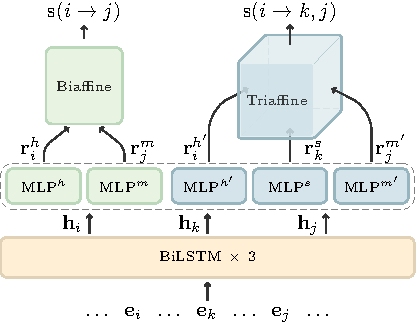
\includegraphics[scale=1.5]{figures/dep-framework.pdf}
	\caption{带二阶扩展的打分方法.}
	\label{fig:dep-framework}
\end{figure}

\subsection{局部头选择训练损失}
Biaffine Parser采用了一个简单的词级别非结构化损失函数,试着对每个词独立最大化正确头的局部概率.
在一个训练实例中,对于一个正确的头-依赖对$(w_i, w_j$),其对应的交叉熵损失为
\begin{equation} \label{eq:biaffine-loss}
	\mathit{L}(i\rightarrow j) = -\log{\frac{\exp(\mathrm{s}(i\rightarrow j))}{\sum_{0 \le i^{\prime} \le n} \exp(\mathrm{s}(i^{\prime}\rightarrow j))}}
\end{equation}
换句话说,模型的训练是基于一个简单的头选择目标,最终所有词的损失都被累加起来,而没有考虑任何树结构的约束.

\subsection{解码方法}
Biaffine Parser将骨干树的搜索和依存弧标签标注视为两个独立的任务.
这里为了方便我们采取了相同的两阶段解析策略.
首先,给定所有依存弧的分值,我们采用复杂度为$O(n^3)$的一阶Eisner算法来寻找最优的骨干句法树.
\begin{equation}
	\label{eq:map-decoding}
	{\boldsymbol{y}}^* = \arg\max_{\boldsymbol{y}} \mathrm{s}(\boldsymbol{x},\boldsymbol{y}) \equiv
	\sum_{i \rightarrow j \in \boldsymbol{y}}{\mathrm{s}(i\rightarrow j)}
\end{equation}
其次,给定最优的无标签骨干树,我们采用局部贪婪分类的方法为树中的每条弧分配一个标签,得到一棵最优的有标签树,具体细节可以参考\citet{dozat-etal-2017-biaffine}.

\begin{figure}[tb]
	\centering
	\begin{subfigure}[b]{0.45\textwidth}
		\centering
		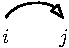
\includegraphics[scale=1.5]{figures/scoring-part/arc.pdf}
		\caption{单弧}
		\label{fig:scoring-part-arc}
	\end{subfigure}
	\begin{subfigure}[b]{0.45\textwidth}
		\centering
		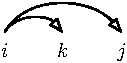
\includegraphics[scale=1.5]{figures/scoring-part/sib.pdf}
		\caption{邻接兄弟}
		\label{fig:scoring-part-sib}
	\end{subfigure}
	\caption{两种打分的子树结构.}
	\label{fig:scoring-part}
\end{figure}

\section{二阶TreeCRF}\label{dep-2o-treecrf}
我们从两方面极大拓展了Biaffine Parser:
使用概率TreeCRF来进行结构化训练,以及显式引入高阶子树的分值.

具体地,我们在基本的一阶模型的基础上引入了二阶邻接兄弟子树的分值:\footnote{
	我们还可以进一步扩展,引入祖父-父亲-孩子的子树分值,然后基于\citet{koo-collins-2010-efficient}提出的$O(n^4)$的Viterbi算法解码.
	这里我们留待作为未来的工作.
}
\begin{equation}\label{eq:dep-2otree-score}
	\mathrm{s}(\boldsymbol{x}, \boldsymbol{y}) = \sum_{i\rightarrow j \in \boldsymbol{y}}\mathrm{s}(i\rightarrow j) + \sum_{
		i\rightarrow \{k,j\} \in \boldsymbol{y}
	} \mathrm{s}(i\rightarrow \{k,j\})
\end{equation}
其中$k$和$j$是$i$的两个相邻的孩子,并且满足$i < k < j$或者$j < k < i$.
图\ref{fig:scoring-part}展示了两种我们要打分的子树结构.

作为一个概率模型,TreeCRF以下面的方式计算一棵树的条件概率
\begin{equation}\label{eq:prob-labeled}
	\begin{split}
		& p(\boldsymbol{y}\mid\boldsymbol{x})  = \frac{\exp(\mathrm{s}(\boldsymbol{x},\boldsymbol{y}))}{Z(\boldsymbol{x}) \equiv \sum_{\boldsymbol{y'} \in \mathcal{Y}(\boldsymbol{x})} {\exp(\mathrm{s}(\boldsymbol{x},\boldsymbol{y'}))}}
	\end{split}
\end{equation}
其中$\mathcal{Y}(\boldsymbol{x})$是输入句子$\boldsymbol{x}$对应所有合法的句法树,$Z(\boldsymbol{x})$通常被称为配分项(partition term).

训练时,TreeCRF应用了下面的损失函数来最大化给定$\boldsymbol{x}$正确句法树$\boldsymbol{y}$的条件概率.
\begin{equation}\label{eq:training-loss-treecrf}
	\begin{split}
		\mathit{L}(\boldsymbol{x},\boldsymbol{y}) &= -\log p(\boldsymbol{y}\mid\boldsymbol{x})  \\
		&= - \mathrm{s}(\boldsymbol{x}, \boldsymbol{y}) + \log Z(\boldsymbol{x})
	\end{split}
\end{equation}

\begin{figure}[tb]
	\centering
	\begin{subfigure}[b]{\textwidth}
		\begin{minipage}{\textwidth}
			\centering
			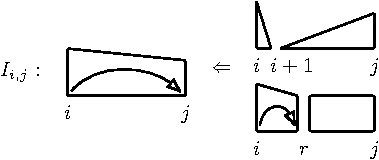
\includegraphics[scale=1.35]{figures/eisner-2o/a.pdf}
			\label{fig:eisner-2o-a}
		\end{minipage}
	\end{subfigure}
	\begin{subfigure}[b]{\textwidth}
		\begin{minipage}{\textwidth}
			\centering
			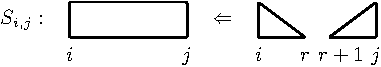
\includegraphics[scale=1.35]{figures/eisner-2o/b.pdf}
			\label{fig:eisner-2o-b}
		\end{minipage}
	\end{subfigure}
	\begin{subfigure}[b]{\textwidth}
		\begin{minipage}{\textwidth}
			\centering
			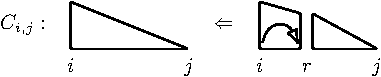
\includegraphics[scale=1.35]{figures/eisner-2o/c.pdf}
			\label{fig:eisner-2o-c}
		\end{minipage}
	\end{subfigure}
	\caption{基于自底向上动态规划的二阶Inside算法图示.}
	\label{fig:eisner-2o}
	% \vspace{-5pt}
\end{figure}

\subsection{基于Triaffine的二阶子树打分}
为了避免对原有打分方法有大的改动,我们采用了一个直接的扩展来获得邻接子树的分值.
首先,我们用三个额外的MLP层来进行和Biaffine所需要的类似的特征提取
\begin{equation}
	\label{mlp-sib}
	\mathbf{r}_i^{h'}; \mathbf{r}_i^{s}; \mathbf{r}_i^{m'} =\mathrm{MLP}^{h'/s/m'} \left( \mathbf{h}_i \right)
\end{equation}
$\mathbf{r}_i^{h'}; \mathbf{r}_i^{s}; \mathbf{r}_i^{m'}$是词$w_i$分别作为头,兄弟,和依赖对应的表示.\footnote{
	另一种方式是重用一阶部分头和依赖的表示,但是我们的前置实验表明这种方法的结果要更差一点
}

然后,我们提出了一个对Biaffine自然的扩展,Triaffine结构,来通过上述的三个向量计算分值\footnote{
	我们同样尝试了\citet{wang-etal-2019-second}的方法,他们用了三个biaffine操作来模拟三个输入向量的交互,但是这种方法的结果相对要差一点.
	篇幅限制我们省略了相应结果的汇报.
}
\begin{equation} \label{eq:triaffine}
	\mathrm{s}(i\rightarrow \{k,j\}) =
	\left[
		\begin{array}{c}
			\mathbf{r}_{k}^{s} \\
			1
		\end{array}
		\right]^\mathrm{T}
	{\mathbf{r}_{i}^{h'}}^\mathrm{T}
	\mathbf{W}^\textit{triaffine}
	\left[
		\begin{array}{c}
			\mathbf{r}_{j}^{m'} \\
			1
		\end{array}
		\right]
\end{equation}
其中$\mathbf{W}^\textit{triaffine} \in \mathbb{R}^{d' \times (d'+1) \times (d'+1)}$是一个三维的张量.
Triaffine可以方便的通过$\mathrm{einsum}$函数在GPU上高效计算.

\subsection{高效的TreeCRF计算方法}

如公式~\ref{eq:training-loss-treecrf}所示,计算TreeCRF损失的关键在于如何计算配分项$Z(\boldsymbol{x})$.
这个问题在前深度学习时代的非神经网络模型上已经被很好的解决了.
我们可以在Viterbi算法的基础上,直接用sum product操作取代max product操作,这样就可以用相同的多项式时间的复杂度得到$Z(\boldsymbol{x})$.
然而,对非神经网络模型而言,由于缺乏自动求导机制,单独的计算Inside算法仍然是不够的.
为了获取边缘概率,然后得到特征权重的梯度,我们还需要实现更加复杂的Outside算法,而这通常要两倍慢于Inside算法.
这可能是TreeCRF在非神经网络上不如Max Margin流行的主要原因.

\begin{algorithm}[tb]
    \begin{algorithmic}[1]
        \newlength{\commentindent}
        \setlength{\commentindent}{.3\textwidth}
        \renewcommand{\algorithmiccomment}[1]{\unskip\hfill\makebox[\commentindent][l]{$\rhd$~#1}\par}
        \LetLtxMacro{\oldalgorithmic}{\algorithmic}
        \renewcommand{\algorithmic}[1][0]{
            \oldalgorithmic[#1]
            \renewcommand{\ALC@com}[1]{
                \ifnum\pdfstrcmp{##1}{default}=0\else\algorithmiccomment{##1}\fi}%
        }
        \STATE \textbf{define:} $I,S,C \in \mathbb{R}^{n \times n \times B}$ \COMMENT{$B$ is \#sents in a batch}
        \STATE \textbf{initialize:} $C_{i, i}  = 0, 0 \le i \le n$

        \FOR [span width]{$w = 1$ \TO $n$}
        \STATE \textbf{Batchify:} $0 \le i$; $j=i+w \le n$
        \STATE $I_{i, j} = \log\left(\exp\left(C_{i, i}  +  C_{j, i+1}\right) ~ +\sum\limits_{i < r < j} \exp\left(I_{i, r} + S_{r, j}+ \mathrm{s}(i, r, j)\right)\right) + \mathrm{s}(i, j)$
        \STATE $S_{i, j} = \log \sum\limits_{i \le r < j} \exp\left(C_{i, r}  +  C_{j, r+1}\right) $ \\
        \STATE $C_{i, j} = \log \sum\limits_{i < r \le j} \exp\left(I_{i, r}  +  C_{r, j}\right)  $ \\
        \ENDFOR \COMMENT{refer to Fig.~\ref{fig:eisner-2o}}
        \RETURN $C_{0, n} \equiv \log Z(\boldsymbol{x})$
    \end{algorithmic}
    \caption{二阶Inside算法.}
    \label{alg:eisner-2o}
\end{algorithm}


据我们所知,所有以前的神经网络上TreeCRF解析的工作都显式地实现了Inside-Outside算法来进行梯度的计算 \citep{zhang-etal-2019-empirical, jiang-etal-2018-supervised}.
为了提升效率,这些计算通常被从GPU迁移到CPU,用Cython加速.

这里我们表明Inside算法可以被高效的批次化,从而充分利用GPU并行计算的能力.
图~\ref{fig:eisner-2o}和算法~\ref{alg:eisner-2o}展示了批次化版本的二阶Inside算法,这是\citet{mcdonald-pereira-2006-online}的二阶Eisner算法的一个直接扩展,将其中的max product操作用sum product取代.
为了简便,我们忽略了自右边位置$j$向左边位置$i$归并生成incomplete/complete/sibling区块的描述.

具体地,对一个批次中$B$个句子,我们首先将不同位置但是相同宽度的区块($i, j$)的分值打包成为一个大的张量.
接着,我们在GPU上通过高效的大规模张量并行操作来同时进行计算和归并.
我们还可以用类似的方式来批次化解码算法,这里省略细节.

值得注意的是,这里描述的技术同样可以在其他形式的文法里应用,比如CKY算法形式的成分句法分析 \citep{finkel-etal-2008-efficient,drozdov-etal-2019-unsupervised}.
具体在章节~\ref{cha:con-crf}中描述.

\subsection{通过反向传播完成的Outside算法}

\citet{eisner-2016-inside}以成分句法分析(短语结构)为例,对反向传播机制和Outside算法的等价性进行了理论证明.
这里我们同样在依存句法上验证了其等价性.

进一步地,我们同样发现边缘概率$p(i \rightarrow j\mid\boldsymbol{x})$直接与对$\log Z(\boldsymbol{x})$关于分值$\mathrm{s}(i\rightarrow j)$的偏导相关,这可以很方便的证明
\begin{equation}
	\label{eq:dep-partial-derivative}
	\begin{split}
		\frac{\partial \log Z}{\partial \mathrm{s}(i\rightarrow j)}
		& = \frac{\partial \log Z}{\partial Z} \cdot \frac{\partial Z}{\partial \mathrm{s}(i\rightarrow j)}\\
		& =\frac{1}{Z} \cdot \frac{\partial \sum_{\boldsymbol{y}} \exp \left(\mathrm{s}(\boldsymbol{x}, \boldsymbol{y}) \right)}{\partial \mathrm{s}(i\rightarrow j)}\\
		& =\frac{1}{Z} \cdot \frac{\partial \sum_{\boldsymbol{y}:i\rightarrow j \in \boldsymbol{{y}}} \exp \left(\mathrm{s}(\boldsymbol{x}, \boldsymbol{y}) \right)}{\partial \mathrm{s}(i\rightarrow j)}\\
		& =\frac{1}{Z} \cdot \frac{\sum_{\boldsymbol{y}:i\rightarrow j \in \boldsymbol{{y}}} \exp \left( \mathrm{s}(\boldsymbol{y}) -\mathrm{s}(i\rightarrow j)  \right)\cdot \partial \exp(\mathrm{s}(i\rightarrow j))}{\partial \mathrm{s}(i\rightarrow j)}\\
		& =\sum_{\boldsymbol{y}:i\rightarrow j \in \boldsymbol{{y}}} \frac{\exp \left( \mathrm{s}(\boldsymbol{y})\right)}{Z}\\
		&= \sum_{\boldsymbol{y}:i\rightarrow j \in \boldsymbol{{y}}} p(\boldsymbol{y}\mid\boldsymbol{x})\\
		&= p(i \rightarrow j\mid\boldsymbol{x})
	\end{split}
\end{equation}
因此偏导数等价于所有包含$i \rightarrow j$的弧的句法树的概率之和,即边缘概率$p(i \rightarrow j\mid\boldsymbol{x})$.
对于TreeCRF分析器,我们可以通过将解码算法中的分值用边缘概率代替,进行\textbf{最小贝叶斯风险}(Minimum Bayesian Risk, MBR)解码 \citep{smith-smith-2007-probabilistic},从而带来一个稳定的提升,相关推导见附录~\ref{cha:mbr-decoding}.

\subsection{局部标注处理}
\label{sub@sec:partial-annotation}

作为一个有吸引力的研究方向,很多研究证明构建或者收集局部标注数据很有效 \citep{nivre-etal-2014-squibs,hwa-1999-supervised,pereira-schabes-1992-inside-outside},在依存句法分析中,一个句子可以关联一个局部标注树.
当结合主动学习(active learning)时,局部标注可以发挥更大的作用,由于只需要标注部分较难的子树结构,这样可以极大减轻标注者的标注负担.
\citet{li-etal-2016-active}中有关于这部分的详细调研.
此外,\citet{peng-etal-2019-overview}最近基于这方面的研究公开了一个局部标注的多领域中文树库.

那么问题就变成了如何利用局部标注数据来训练模型.
\citet{li-etal-2016-active}基于这个目的提出扩展TreeCRF到局部标注场景,并在非神经网络模型上取得了不错的效果.
这里我们借鉴他们的研究到了神经网络模型中.
我们尤其关注于在结构化学习和高阶建模上利用局部标注数据.

对基本的基于一阶局部训练方法的Biaffine Parser来说,利用局部标注最直接的方式是忽略未标注的词.
与此相对的是,树结构约束允许标注弧影响未标注词的概率分布,并且高阶建模进一步促进了词之间的交互.
因此,直觉上结构化学习和高阶建模都是非常有用的.

对于局部标注,我们和\citet{li-etal-2016-active}一样,定义训练的目标函数如下:
\begin{equation}
	\label{eq:training-loss-treecrf-partial}
	\begin{split}
		\mathit{L}(\boldsymbol{x}, {\boldsymbol{y}^p}) &= -\log \sum\limits_{\boldsymbol{y} \in \mathcal{Y}(\boldsymbol{x}); \boldsymbol{y} \supseteq {\boldsymbol{y}^p}} p(\boldsymbol{y}\mid\boldsymbol{x})  \\
		&= - \log \frac{Z(\boldsymbol{x}, {\boldsymbol{y}^p}) \equiv \sum\limits_{\boldsymbol{y} \in \mathcal{Y}(\boldsymbol{x}); \boldsymbol{y} \supseteq \boldsymbol{y}^p} \exp(\mathrm{s}(\boldsymbol{x},\boldsymbol{y}))}{Z(\boldsymbol{x})}
	\end{split}
\end{equation}
其中$Z(\boldsymbol{x}, {\boldsymbol{y}^p})$ 只包含所有与给定局部标注树兼容的句法树,并且可以用和$Z(\boldsymbol{x})$类似的方式进行高效的计算.

\begin{figure}[tb]
	\centering
	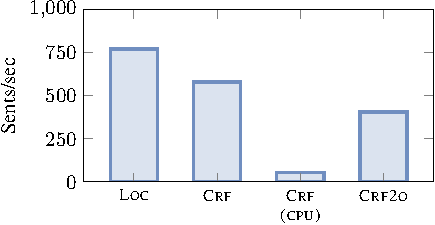
\includegraphics[scale=1.2]{figures/dep-speed.pdf}
	\caption{
		PTB的test数据上的速度比较.
	}
	\label{fig:speed}
\end{figure}

\section{实验结果及分析}\label{sec:dep-exps}

\begin{table}[tb!]
  \centering
  \begin{tabular}{llcccc}
    \toprule
                             &                        & \multicolumn{2}{c}{Dev} & \multicolumn{2}{c}{Test}                                                                       \\
                             &                        & UAS                     & LAS                      & UAS                              & LAS                              \\[2pt]
    \hline
    \\[-15pt]
    \multirow{10}{*}{PTB}    & Biaffine17             & -                       & -                        & 95.74                            & 94.08                            \\
                             & F\&K19                 & -                       & -                        & -                                & 91.59                            \\
    %    \cite{ma-hovy-2017-neural}        & 94.88 & 92.98 \\
    %    \cite{ma-etal-2018-stack}         & 95.87 & 94.19 \\
                             & Li19                   & 95.76                   & 93.97                    & 95.93                            & 94.19                            \\
                             & Ji19                   & 95.88                   & 93.94                    & 95.97                            & 94.31                            \\
                             & Zhang19                & -                       & -                        & -                                & 93.96                            \\[3pt]
                             & \textsc{Loc}           & 95.82                   & 93.99                    & 96.08                            & 94.47                            \\
                             & \textsc{Crf} w/o MBR   & 95.74                   & 93.96                    & 96.04                            & 94.34                            \\
                             & \textsc{Crf}           & 95.76                   & 93.99                    & 96.02                            & 94.33                            \\
                             & \textsc{Crf2o} w/o MBR & \textbf{95.92}          & \textbf{94.16}           & \textbf{96.14}                   & \textbf{94.49}                   \\
                             & \textsc{Crf2o}         & 95.90                   & 94.12                    & 96.11                            & 94.46                            \\[2pt]
    \hline
    \\[-15pt]
    \multirow{7}{*}{CoNLL09} & Biaffine17             & -                       & -                        & 88.90                            & 85.38                            \\
                             & Li19                   & 88.68                   & 85.47                    & 88.77                            & 85.58                            \\[3pt]
                             & \textsc{Loc}           & 89.07                   & 86.10                    & 89.15                            & 85.98                            \\
                             & \textsc{Crf} w/o MBR   & 89.04                   & 86.04                    & 89.14                            & 86.06                            \\
                             & \textsc{Crf}           & 89.12                   & 86.12                    & 89.28                            & 86.18\rlap{$^\dagger$}           \\
                             & \textsc{Crf2o} w/o MBR & 89.29                   & 86.24                    & 89.49                            & 86.39                            \\
                             & \textsc{Crf2o}         & \textbf{89.44}          & \textbf{86.37}           & \textbf{89.63}\rlap{$^\ddagger$} & \textbf{86.52}\rlap{$^\ddagger$} \\[2pt]
    \hline
    \\[-15pt]
    \multirow{5}{*}{NLPCC19} & \textsc{Loc}           & 77.01                   & 71.14                    & 76.92                            & 71.04                            \\
                             & \textsc{Crf} w/o MBR   & 77.40                   & 71.65                    & 77.17                            & 71.58                            \\
                             & \textsc{Crf}           & 77.34                   & 71.62                    & 77.53\rlap{$^\ddagger$}          & 71.89\rlap{$^\ddagger$}          \\
                             & \textsc{Crf2o} w/o MBR & 77.58                   & 71.92                    & 77.89                            & 72.25                            \\
                             & \textsc{Crf2o}         & \textbf{78.08}          & \textbf{72.32}           & \textbf{78.02}\rlap{$^\ddagger$} & \textbf{72.33}\rlap{$^\ddagger$} \\
    \bottomrule
  \end{tabular}
  \caption{主要结果. 我们在test上基于\textsc{Loc}做显著性检验,其中``$\dagger$''代表$\mathrm{p} < 0.05$,``$\ddagger$''代表$\mathrm{p} < 0.005$.
    Biaffine17: \cite{dozat-etal-2017-biaffine}; F\&K19: \cite{falenska-kuhn-2019-non};
    Li19: \cite{li-etal-2019-attentive}; Ji19: \cite{ji-etal-2019-graph};
    Zhang19: \cite{zhang-etal-2019-empirical}.
  }
  \label{table:dev-test}
\end{table}




\noindent\textbf{参数设置.}
我们直接采用了\citet{dozat-etal-2017-biaffine}的大部分参数设置,包含Dropout和初始化策略.
对于CharLSTM,和\citet{lample-etal-2016-neural}一样,输入字向量的维度是50,输出向量的维度是100.
对于二阶模型,我们设置$\mathbf{r}^{h'/s/m'}_i$的维度为100(进一步提升到300带来的提升很小).
我们训练模型最多1,000次迭代,并且如果在dev上的性能连续100次不提升那就停止训练.

\noindent\textbf{模型定义.}
\textsc{Loc}使用了局部交叉熵训练损失函数,并且解码时使用Eisner算法来获取最优的投影树.
\textsc{Crf}和\textsc{Crf2o}各自代表一阶和二阶TreeCRF模型.
$\textsc{Loc}^{\textsc{mst}}$代表基本的基线模型,但是解码时采用和\citet{dozat-etal-2017-biaffine}一样的MST算法输出非投影树.

\subsection{效率比较}

图~\ref{fig:speed}在PTB的测试集上比较了不同模型的解析速度.
为了能够公平比较,我们在相同的机器上运行所有的模型,模型的配置为Intel Xeon CPU (E5-2650v4, 2.20GHz)以及GeForce GTX 1080 Ti GPU.
``\textsc{Crf (cpu)}''表示直接在CPU运算Inside-Outside算法上,并利用Cython加速的模型.
由于句子间是相互独立的,因此这里还利用的多线程.
我们一共用了4个线程,并且进一步增加没有更多的提升速度.

可以看到通过批次化Inside算法以及用自动求导机制的反向传播代替Outside算法这两方面的改进,TreeCRF效率被极大的提升了.
对于\textsc{Crf}模型,我们的实现可以解析超过500句每秒,大约十倍快于多线程的``\textsc{Crf (cpu)}''.
对于二阶的\textsc{Crf2o},我们的分析器达到了400句每秒的速度,达到了实时系统的需求.

\subsection{主要结果}

表~\ref{table:dev-test}列出了Dev和Test数据上的结果.
两个数据上的结果趋势大部分是一致的.
为了能够与前人的结果公平比较,我们只比较了不利用外部资源的工作,例如ELMo \citep{peters-etal-2018-deep}或BERT \citep{devlin-etal-2019-bert}.
可以看到我们的基线模型\textsc{Loc}在PTB和CoNLL09相较于前人达到了最好的性能

在PTB上,\textsc{Crf}和\textsc{Crf2o}没有能够进一步提升解析准确率,这部分是由于这两个数据上的结果已经很高了.
然而,正如章节\ref{sub@sec:dep-analysis}所示,结构化学习和高阶建模仍然带来了一些正面的影响.

\textsc{Crf}在CoNLL09上显著超越了\textsc{Loc},并且\textsc{Crf2o}可以进一步提升性能.

在局部标注数据NLPCC19上,\textsc{Crf}极大的超过了\textsc{Loc},这表明了结构化学习在局部标注场景下的有效性.
\textsc{Crf2o}通过显式地建模二阶子树的特征,进一步的提升了解析性能.
这些结果验证了我们在章节~\ref{sub@sec:partial-annotation}的直觉性讨论.
需要注意的是,局部标注的结果看起来比较低,这里的原因是局部标注的词通常来说对于模型都是比较难的.

\subsection{分析}
\label{sub@sec:dep-analysis}

\begin{figure*}[tb!]
	\centering
	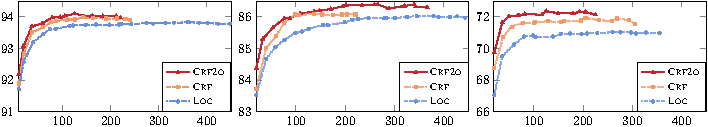
\includegraphics[width=\textwidth]{figures/convergency.pdf}
	\caption{
		PTB、CoNLL09和NLPCC19的dev数据的训练收敛曲线(LAS相对于训练迭代次数).}
	\label{fig:convergency}
\end{figure*}

\noindent\textbf{MBR解码的影响.}
对于\textsc{Crf}和\textsc{Crf2o},我们默认进行MBR解码,也就是直接在边缘概率上应用Eisner算法 \citep{smith-smith-2007-probabilistic}来找到最优的句法树.
\begin{equation}
	\begin{split}
		& {\boldsymbol{y}}^* = \arg\max_{\boldsymbol{y}} \sum_{i \rightarrow j \in \boldsymbol{y}}{p(i \rightarrow j\mid\boldsymbol{x})}
	\end{split}
\end{equation}
表~\ref{table:dev-test}报告了MAP解码(即根据依存分值直接寻找最优句法树,关于与MBR解码的联系详见附录~\ref{cha:mbr-decoding}).
除了PTB数据集的结果已经比较高了之外,MBR解码对于\textsc{Crf}和\textsc{Crf2o}都带来了不多但是一致的提升.

\noindent\textbf{收敛行为.}
图~\ref{fig:convergency}比较了不同模型的收敛曲线.
清晰起见,我们每20次迭代选择一个结果最高的数据点放入到图里面.
可以明显看到,结构化学习和高阶建模都带来了一致的提升.
\textsc{Crf2o}稳定的达到了最好的结果,并且收敛要远远快于基本的\textsc{Loc}.

\begin{table}[tb!]
    \setlength{\tabcolsep}{5pt}
    \centering
    \begin{tabular}{llccccc}
        \toprule
                                 &                & \multicolumn{3}{c}{SIB} & \multirow{2}{*}{UCM} & \multirow{2}{*}{LCM}                                   \\
                                 &                & P                       & R                    & F                                                      \\[2pt]
        \hline
        \\[-15pt]
        \multirow{3}{*}{PTB}     & \textsc{Loc}   & 91.16                   & 90.80                & 90.98                & 61.59          & 50.66          \\
                                 & \textsc{Crf}   & 91.24                   & 90.92                & 91.08                & 61.92          & 50.33          \\
                                 & \textsc{Crf2o} & \textbf{91.56}          & \textbf{91.11}       & \textbf{91.33}       & \textbf{63.08} & \textbf{50.99} \\[2pt]
        \hline
        \\[-15pt]
        \multirow{3}{*}{CoNLL09} & \textsc{Loc}   & 79.20                   & 79.02                & 79.11                & 40.10          & 28.91          \\
                                 & \textsc{Crf}   & 79.17                   & 79.55                & 79.36                & 40.61          & 29.38          \\
                                 & \textsc{Crf2o} & \textbf{81.00}          & \textbf{80.63}       & \textbf{80.82}       & \textbf{42.53} & \textbf{30.09} \\
        \bottomrule
    \end{tabular}
    \caption{test数据上子树和完全树的结果.}
    \label{table:dev-test-subtree}
\end{table}

\noindent\textbf{子树和完全树的结果.}
除了弧级别的准确率(UAS/LAS),我们还希望能够评估模型在子树和完全树上的性能.
表~\ref{table:dev-test-subtree}展示了相关的结果.
这里我们忽略了局部标注的NLPCC19数据.
UCM(Unlabeled Complete Match)代表无标签完全匹配率,即所有对应无标签树完全正确的句子的比率,而LCM进一步要求树上的所有标签也是正确的.

对于SIB,我们评估了模型在邻接兄弟子树上的结果(系统输出和对应的正确子树).
根据公式~\ref{eq:dep-2otree-score},当且仅当词$w_k$和词$w_j$都是词$w_i$的同侧孩子,并且没有其他词$w_i$的孩子在这两者之间,才称$i\rightarrow \{k,j\}$ 是一个邻接兄弟子树.
给定两棵树,我们可以收集所有的邻接兄弟子树,然后组成一个三元组集合.
之后我们评估相应的P/R/$\mathrm{F}_1$值.
请注意在局部标注下评估SIB是做不到的.

可以明显看到,通过建模邻接兄弟子树的分值,SIB的性能相比于\textsc{Crf}和\textsc{Loc}得到了更大的提升,并且这进一步带来了在完全树匹配率(UCM/LCM)上的进步.

\begin{figure}[tb!]
	\centering
	\begin{subfigure}[b]{0.4\textwidth}
		\centering
		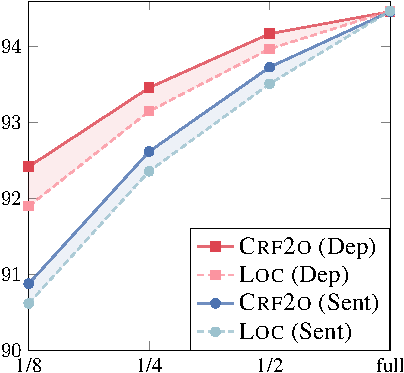
\includegraphics[width=1.\textwidth]{figures/part-gap-ptb.pdf}
	\end{subfigure}
	\begin{subfigure}[b]{0.4\textwidth}
		\centering
		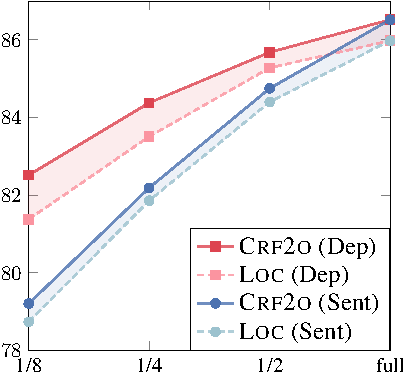
\includegraphics[width=1.\textwidth]{figures/part-gap-conll.pdf}
	\end{subfigure}
	\caption{
		PTB(左)和CoNLL09(右)的测试集有关训练数据量(弧数以及句子数)变化之后的LAS比较.
	}
	\label{fig:part-gap}
\end{figure}

\noindent\textbf{学习局部标注树的能力.}
为了更好的理解为什么\textsc{Crf2o}在局部标注的NLPCC19上表现的比较好,我们通过随机丢弃一定比例的训练数据来进行了更多的比较实验.
我们要么随机丢弃了一部分的句子(完全树),要么每个句子随机丢弃一部分弧(局部树).
图~\ref{fig:part-gap}列出了结果.

可以看到当我们渐渐地丢弃一定数量的训练句子的时候,性能差距相当稳定.
与此相反的是,当每个训练句子有更少的标注弧时,性能差距明显变得更大了.
这表明\textsc{Crf2o}在利用局部标注数据训练模型上要优于\textsc{Loc}.

\begin{table*}[tb]
    \setlength{\tabcolsep}{3.3pt}
    \centering
    \caption{UD2.2和UD2.3的test数据的LAS结果.
        同样地,$\dagger$和$\ddagger$各自表示基于\textsc{Loc}分析器,$p<0.05$以及$p<0.005$的显著性级别. }
    \begin{tabularx}{\textwidth}{lccccccccccccc}
        \toprule
                                      & bg             & ca             & cs                               & de                              & en                              & es                               & fr                              & it                               & nl                               & no                              & ro                               & ru                               & Avg.                             \\[1pt]
        \hline
        \\[-15pt]
        \multicolumn{14}{c}{UD2.2}                                                                                                                                                                                                                                                                                                                                                                                                                                   \\[1pt]
        $\textsc{Loc}_{\textsc{mst}}$ & 90.44          & 91.11          & 91.04                            & 80.21                           & 86.86                           & 90.67                            & 87.99                           & 91.19                            & 88.24                            & 90.35                           & 86.24                            & 93.01                            & 88.95                            \\
        \textsc{Loc}                  & 90.45          & 91.14          & 90.97                            & 80.02                           & 86.83                           & 90.56                            & 87.76                           & 91.14                            & 87.72                            & 90.74                           & 86.20                            & 93.01                            & 88.88                            \\
        \textsc{Crf}                  & 90.73          & 91.25          & 91.01                            & \textbf{80.56}\rlap{$^\dagger$} & 86.92                           & 90.81\rlap{$^\dagger$}           & \textbf{88.16}                  & 91.64\rlap{$^\dagger$}           & 88.10                            & 90.85                           & 86.50                            & 93.17\rlap{$^\dagger$}           & 89.14\rlap{$^\ddagger$}          \\
        \textsc{Crf2o}                & \textbf{90.77} & \textbf{91.29} & \textbf{91.54}\rlap{$^\dagger$}  & 80.46                           & \textbf{87.32}\rlap{$^\dagger$} & \textbf{90.86}\rlap{$^\dagger$}  & 87.96                           & \textbf{91.91}\rlap{$^\ddagger$} & \textbf{88.62}\rlap{$^\ddagger$} & \textbf{91.02}\rlap{$^\dagger$} & \textbf{86.90}\rlap{$^\ddagger$} & \textbf{93.33}\rlap{$^\ddagger$} & \textbf{89.33}\rlap{$^\ddagger$} \\[1pt]
        \multicolumn{14}{c}{using raw text}                                                                                                                                                                                                                                                                                                                                                                                                                          \\[1pt]
        Ji19                          & 88.28          & 89.90          & 89.85                            & 77.09                           & 81.16                           & 88.93                            & 83.73                           & 88.91                            & 84.82                            & 86.33                           & 84.44                            & 86.62                            & 85.83                            \\
        \textsc{Crf2o}                & \textbf{89.72} & \textbf{91.27} & \textbf{90.94}                   & \textbf{78.26}                  & \textbf{82.88}                  & \textbf{90.79}                   & \textbf{86.33}                  & \textbf{91.02}                   & \textbf{87.92}                   & \textbf{90.17}                  & \textbf{85.71}                   & \textbf{92.49}                   & \textbf{88.13}                   \\
        \hline
        \\[-15pt]
        \multicolumn{14}{c}{UD2.3}                                                                                                                                                                                                                                                                                                                                                                                                                                   \\[1pt]
        $\textsc{Loc}_{\textsc{mst}}$ & 90.56          & 91.03          & 91.98                            & 81.59                           & 86.83                           & 90.64                            & 88.23                           & 91.67                            & 88.20                            & 90.63                           & 86.51                            & 93.03                            & 89.23                            \\
        \textsc{Loc}                  & 90.57          & 91.10          & 91.85                            & 81.68                           & 86.54                           & 90.47                            & 88.40                           & 91.53                            & 88.18                            & 90.65                           & 86.31                            & 92.91                            & 89.19                            \\
        \textsc{Crf}                  & 90.52          & \textbf{91.19} & 92.02                            & 81.43                           & 86.88\rlap{$^\dagger$}          & 90.76\rlap{$^\dagger$}           & 88.75                           & 91.76                            & 88.08                            & \textbf{90.79}                  & 86.54                            & 93.16\rlap{$^\ddagger$}          & 89.32\rlap{$^\ddagger$}          \\
        \textsc{Crf2o}                & \textbf{90.76} & 91.12          & \textbf{92.15}\rlap{$^\ddagger$} & \textbf{81.94}                  & \textbf{86.93}\rlap{$^\dagger$} & \textbf{90.81}\rlap{$^\ddagger$} & \textbf{88.83}\rlap{$^\dagger$} & \textbf{92.34}\rlap{$^\ddagger$} & \textbf{88.21}\rlap{$^\dagger$}  & 90.78                           & \textbf{86.62}                   & \textbf{93.22}\rlap{$^\ddagger$} & \textbf{89.48}\rlap{$^\ddagger$} \\
        \multicolumn{14}{c}{using gold POS tags}                                                                                                                                                                                                                                                                                                                                                                                                                     \\[1pt]
        Zhang19                       & 90.15          & 91.39          & 91.10                            & 83.39                           & 88.52                           & 90.84                            & 88.59                           & 92.49                            & 88.37                            & 92.82                           & 84.89                            & 93.11                            & 89.85                            \\
        \textsc{Crf2o}                & \textbf{91.32} & \textbf{92.57} & \textbf{92.66}                   & \textbf{84.56}                  & \textbf{88.98}                  & \textbf{91.88}                   & \textbf{89.83}                  & \textbf{92.94}                   & \textbf{89.85}                   & \textbf{93.26}                  & \textbf{87.39}                   & \textbf{93.86}                   & \textbf{90.76}                   \\
        \bottomrule
    \end{tabularx}
    \label{table:ud-test}
\end{table*}



\subsection{多语言UD数据集上的结果}

表~\ref{table:ud-test}比较了UD数据上不同模型的结果.
在UD数据中包含了大量的非投影树.
我们采用了\citet{nivre-nilsson-2005-pseudo}的伪投影方法来将许多语言中大量存在的非投影树转换为投影树.
基本的想法是将非投影树转换为投影树的时候利用更多更复杂的标签来标记,以方便后处理的时候能够恢复.

可以看到在基础的局部模型上,直接的基于MST算法的非投影解析方法$\textsc{Loc}^{\textsc{mst}}$和伪投影方法\textsc{Loc}达到了非常相似的性能.

更重要的是,\textsc{Crf}和\textsc{Crf2o}在大部分语言上相比于基线模型都出现了一致的提升.
在UD2.2和UD2.3上,我们提出的\textsc{Crf2o}模型在12个语言中的10个上达到了最高的解析准确率,并且在超过7个语言上获得的提升是显著的.
总体上,平均分别在UD2.2和UD2.3各自达到了0.45和0.29的提升,这同样是显著的($p<0.005$).

在UD2.2上,我们和CoNLL18任务一样采用的是毛文本,并且我们的\textsc{Crf2o}分析器上比\citet{ji-etal-2019-graph}平均要高2.30.
在UD2.3上,\citet{zhang-etal-2019-empirical}使用了正确词性作为输入,我们平均比他们高0.91.
需要注意的是\citet{ji-etal-2019-graph}里德语(\textsc{De})结果错误地使用了正确的句子分割,符号化以及词性,而表中的结果是用了预测的词性,并重新运行他们的分析器得到的.
我们的\textsc{Crf2o}分析器在使用他们的词性之后平均的LAS达到了87.64.

\section{本章小结}
\label{sec:dep-conclusions}

本章首次在神经依存句法分析模型上提出了一个二阶TreeCRF的扩展,并提出使用Triaffine结构来为二阶子树打分.
我们提出了批次化的Inside算法,以适应在GPU上的并行运算.
我们同样从经验上验证了复杂的Outside算法可以隐式地通过高效的自动求导机制来完成,相应可以自然地产生梯度以及边缘概率.
我们在13个语言的27个数据集上进行了大量的实验和详尽的分析,发现结构化学习和高阶建模可以进一步地从不同的方面提升当前最佳的Biaffine Parser:1)更好的收敛行为;2)在子树和完全树上更优越的性能;3)对局部标注数据更好的利用.

\chapter{基于树形条件随机场的快速精准成分句法分析}
\label{cha:con-crf}

本章节提出了一个基于树状条件随机场的快速精准的神经成分句法分析器.
估计概率分布一直是自然语言处理领域的一个核心问题.
但是,在深度学习时代和前深度学习时代,不同于线性链条件随机场(linear chain CRF)在序列标注任务中的大量应用,由于Inside-Outside算法的高复杂度,还很少有工作将树形条件随机场应用到成分句法分析任务当中.
这里我们提出应用树状条件随机场到成分句法分析,核心的想法是批次化计算损失函数用到的Inside算法,使其能够支持在GPU上的大规模张量并行计算,与此同时结合基于高效自动求导机制的反向传播,避免了复杂的Outside算法的计算.
我们同样提出一个简单的两阶段解析方法,bracketing-then-labeling,来进一步提升分析器的效率.
为了提升解析的性能,受依存句法分析器的启发,我们引入了一个基于边界表示和仿射注意力的新打分架构,以及一个有效的Dropout策略.
在PTB、CTB5.1和CTB7上的实验表明我们的两阶段条件随机场分析器在使用和不使用BERT的两种设置上,达到了新的最佳性能,并且解析速度达到了1,000句每秒.

\section{引言}\label{sec:con-intro}

\begin{figure}[tb!]
	\centering
	\begin{subfigure}[b]{0.45\textwidth}
		\centering
		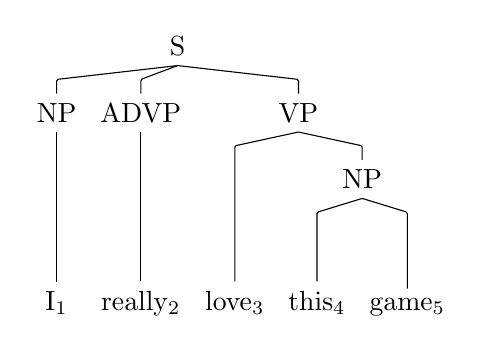
\begin{tikzpicture} [
				level distance=24pt,
				every tree node/.style={align=center,anchor=base},
				frontier/.style={distance from root=92pt},
				edge from parent/.style={draw,edge from parent path={(\tikzparentnode.south) {[rounded corners=0.5pt]-- ($(\tikzchildnode |- \tikzparentnode.south) + (0, -5pt)$) -- (\tikzchildnode)}}}
			]
			\Tree
			[.S
				[.NP I$_1$ ]
				[.ADVP really$_2$ ]
				[.VP love$_3$ [.NP this$_4$ game$_5$ ] ]
			];
		\end{tikzpicture}
		\caption{原始句法树}
		\label{fig:con-original-tree}
	\end{subfigure}
	\hfill
	\begin{subfigure}[b]{0.45\textwidth}
		\centering
		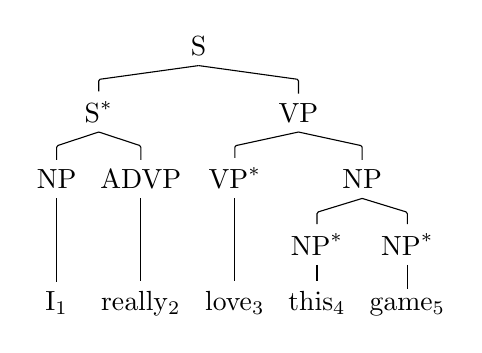
\begin{tikzpicture} [
				level distance=24pt,
				every tree node/.style={align=center,anchor=base},
				frontier/.style={distance from root=92pt},
				edge from parent/.style={draw,edge from parent path={(\tikzparentnode.south) {[rounded corners=0.5pt]-- ($(\tikzchildnode |- \tikzparentnode.south) + (0, -5pt)$) -- (\tikzchildnode)}}}
			]
			\Tree
			[.S
				[.$\textrm{S}^\ast$ [.NP I$_1$ ] [.ADVP really$_2$ ] ]
				[.VP
					[.$\textrm{VP}^\ast$ love$_3$ ]
					[.NP [.$\textrm{NP}^\ast$ this$_4$ ] [.$\textrm{NP}^\ast$ game$_5$ ] ]
				]
			];
		\end{tikzpicture}
		\caption{遵循乔姆斯基范式的左二叉化句法树}
		\label{fig:con-binaried-tree}
	\end{subfigure}
	\caption{
		成分句法树的例子.
		其中词性在这里被忽略
	}
	\label{fig:con-tree-full-figure}
\end{figure}

给定一个句子,成分句法分析旨在构建一个层次化的树结构. 如图\ref{fig:con-tree-full-figure},其中每个叶子结点是输入句子的每个词,而非终端结点作为区块(Constituents),如\texttt{$VP_{3,5}$}.

成分句法分析是自然语言处理领域一个基础但是富有挑战性的任务.
由于诸如宾州树库(Penn Treebank,PTB)、中文宾州树库(Penn Chinese Treebank,CTB)等大规模树库的标注,成分句法分析吸引了一大批研究者的关注.
同样的,句法分析输出的句法树也被证明对于大量的下游任务\cite{akoury-etal-2019-syntactically,wang-etal-2018-tree}都有用.

作为最有影响力的工作之一,\cite{collins-1997-three}概率上下文无关文法 (Probabilistic Context-Free Grammars,PCFGs)扩展到了词汇化文法(Lexicalized PCFGs).
由此开始,成分句法分析方法一直是这样的生成式模型(generative models)占据主导地位,并且其中广泛使用的Berkeley Parser采用了带隐式非终端结点标注的非词汇化概率上下文无关文法(Unlexicalized PCFGs)\cite{matsuzaki-etal-2005-probabilistic,petrov-klein-2007-improved}.
而在判别式方法(discriminative models),存在着两种主要方向.
第一种采取了以动态规划解码为基础的基于图的方法,训练时使用局部max-entropy估计\cite{kaplan-etal-2004-speed}或者全局max-margin方法\cite{taskar-etal-2004-max}.
第二类则通过基于贪婪解码或者集束搜索(beam search)产生shift-reduce这样的转移序列来构建一棵树,这种方法被称为基于转移的方法\cite{sagae-lavie-2005-classifier,zhu-etal-2013-fast}.

最近,得益于深度神经网络在上下文表示方面令人印象深刻的发展,成分句法分析取得了显著的进展.
其中,\cite{cross-huang-2016-span}的基于转移的分析器,以及\cite{stern-etal-2017-minimal}的基于图的分析器是两个具有代表性的工作.
作为判别式模型,两个分析器有很多的共同点,他们都使用了1)多层双向LSTM作为编码器;2)从双向LSTM的输出得到的minus features作为区块的表示;3)利用MLP层来为区块打分;4)max-margin的训练损失函数.
后续的大多数工作\cite{gaddy-etal-2018-whats,kitaev-klein-2018-constituency}的主要设置都和这两个分析器一样, 并且都相比传统的非神经网络模型达到了更好的准确率,这特别是得益于由在大规模无标记文本上训练的语言模型输出的上下文词表示的使用\cite{peters-etal-2018-deep,devlin-etal-2019-bert}.

然而尽管有这些显著的进展,现有的成分句法分析的研究仍然受两个相互关联的缺点困扰.
首先,解析速度(训练速度同理)很慢,并且很难满足现实系统的需要.
其次,显式的树/子树概率建模的缺失一定程度上影响来分析器输出的利用.
一方面,估计概率分布一直是自然语言处理领域的核心问题\cite{le-zuidema-2014-inside}.
另一方面,与没有上下姐的树的分值相比,树的概率可以作为一种软特征,更好的被更高层级的任务所利用\cite{jin-etal-2020-relation},且子树的边缘概率可以支持更加复杂的最小贝叶斯风险解码\cite{smith-smith-2007-probabilistic}.

事实上,\cite{finkel-etal-2008-efficient,durrett-klein-2015-neural}都通过建模树的条件概率$p(\boldsymbol{t}\mid\boldsymbol{x})$,提出了基于CRF\cite{lafferty-etal-2001-crf}的成分句法分析器.
但是,由于损失函数和梯度计算需要的Inside-Outside算法的高复杂度(尤其是Outside算法),这些模型都极端低效.
而在深度学习时代,由于以前所有的工作都直接在CPU上运行Inside-Outside算法,而让模型频繁在CPU和GPU切换所需要的时间代价是昂贵的,因此效率问题变得更加严重.

本章节通过极大拓展\cite{stern-etal-2017-minimal}的基于图的分析器,提出了一个CRF成分句法分析器.
主要的贡献在于我们为损失函数和梯度能够在GPU上能够直接计算,类似于章节\ref{cha:dep-crf},我们提出了Inside算法的批次化方法.
与此同时,我们发现Outside算法的可以通过自动的反向传播机制被高效的完成,这验证了\cite{eisner-2016-inside}出色的理论性能做,使得outside过程与Inside一样高效.
类似的,我们也批次化了CKY(Cocke–Kasami–Younger)算法,以支持高效的解码.

总体而言,我们做了如下的贡献.
\begin{itemize}
    \item 为了直接建模树和子树的概率,我们首次提出了一个快速精准的CRF成分句法分析器.
          通过批次化技术支持Inside算法和CKY算法在GPU上的直接计算,长期以来一直困扰句法分析社区的效率问题在这里被很好的解决了.

    \item 我们提出了一个两阶段的解析方法bracketing-then-labeling:先产生无标记树骨干树(bracketing)再标注标签(labeling)的解析方法,这不仅更加高效,并且达到了比一阶段解析方法稍好的性能.

    \item 我们提出了基于区块表示的一个新的打分架构,以及基于仿射注意力机制的打分方法,比minus-feature方法表现的更好.
          我们同样表明,通过更好的模型及参数设置,比如Dropout,解析的性能可以被极大提升.

    \item 在中英文的三个基准数据集上的实验表明,我们提出的两阶段解析方法在使用BERT和不使用BERT\cite{devlin-etal-2019-bert})的两种设置下,性能上达到了新的最佳水准.
          解析速度方面,我们的分析器可以达到1,000句每秒的解析速度.
\end{itemize}

\begin{figure}[tb]
    \centering
    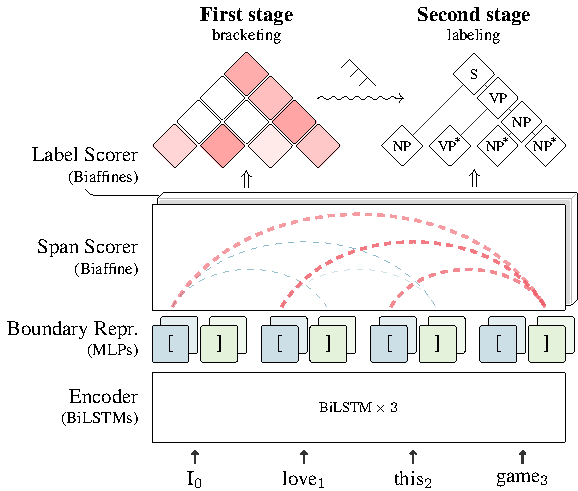
\includegraphics [scale=1.2]{figures/con-framework.pdf}
    \caption{模型架构.}
    \label{fig:con-framework}
\end{figure}

\section{两阶段CRF解析}\label{sec:2stage-parsing}

正式地,给定一个由$n$个词组成的句子$\boldsymbol{x}=w_0,\dots,w_{n-1}$,如图~\ref{fig:con-tree-original}所示,一棵成分句法树可以表示为$\boldsymbol{t}$,其中$(i,j,l) \in \boldsymbol{t}$是一个包含$w_{i}...w_{j}$的区块,对应的句法标签为$l \in \mathcal{L}$.
一棵树同样可以被分解为两个部分,即,$\boldsymbol{t}=(\boldsymbol{y}, \boldsymbol{l})$,其中$\boldsymbol{y}$是一棵无标签树(又称为bracketed tree),而$\boldsymbol{l}$是树中所有区块的标签按一定顺序产生的标签序列.
区块$(3,5,\texttt{VP})$可以等价表示为$\texttt{VP}_{3,5}$.

为了能够适应Inside算法和CKY算法,我们用NLTK工具包\footnote{\url{https://www.nltk.org}}将原始的树转换为了遵循乔姆斯基范式(Chomsky Normal Form,CNF)的二叉树形式,如图~\ref{fig:con-binaried-tree}所示.
特别地,连续的单链产生式被压缩为了一个标签,比如$\texttt{X}_{i,j} \rightarrow \texttt{Y}_{i,j}$会被压缩为一个$\texttt{X+Y}_{i,j}$.
根据前置实验,我们在二叉化原始树的时候,采用了左二叉.
在用CKY解码获得一棵最佳的树之后,CNF树会被恢复为原来的\textit{n}-ary形式.

\subsection{模型定义}\label{sub@sec:model-definition}

在这份工作中,我们对成分句法分析采用了一个两阶段的解析框架bracketing-then-labeling.
这与传统的一阶段解析方法\cite{stern-etal-2017-minimal,gaddy-etal-2018-whats}相比,不仅简化了模型架构,同样也提升了效率.

\noindent\textbf{第一阶段:bracketing.}
给定句子$\boldsymbol{x}$,第一阶段的目标是找到一个最优的无标签树$\boldsymbol{y}$.
一棵树的分值被分解为所有包含的区块的分值.
\begin{equation} \label{eq:tree-score}
    \mathrm{s}(\boldsymbol{x},\boldsymbol{y}) = \sum\limits_{(i,j)\in \boldsymbol{y}}\mathrm{s}(i,j)
\end{equation}
对于CRF,条件概率为
\begin{equation}\label{eq:tree-prob}
    \begin{split}
        & p(\boldsymbol{y}\mid\boldsymbol{x})  = \frac{\exp({\mathrm{s}(\boldsymbol{x},\boldsymbol{y}))}}{Z(\boldsymbol{x}) \equiv \sum\limits_{\boldsymbol{y'} \in \mathcal{Y}(\boldsymbol{x})} {\exp({\mathrm{s}(\boldsymbol{x},\boldsymbol{y'}))}}}
    \end{split}
\end{equation}
其中$Z(\boldsymbol{x})$被称为partition term,$\mathcal{Y}(\boldsymbol{x})$是输入句子$\boldsymbol{x}$对应的所有合法句法树的集合.

给定所有的区块分值$\mathrm{s}(i,j)$,我们可以用CKY算法来找到一棵最优的无标签句法树$\hat{\boldsymbol{y}}$.
\begin{equation} \label{eq:tree-argmax}
    \hat{\boldsymbol{y}} = \arg\max_{\boldsymbol{y}} \mathrm{s}(\boldsymbol{x}, \boldsymbol{y}) = \arg\max_{\boldsymbol{y}} p(\boldsymbol{y} \mid \boldsymbol{x})
\end{equation}

\noindent\textbf{第二阶段:labeling.}
给定一个句子$\boldsymbol{x}$和一棵树$\boldsymbol{y}$,第二阶段独立地给每个区块$(i,j) \in \boldsymbol{y}$预测一个标签.
\begin{equation} \label{eq:label-argmax}
    \hat{l} = \arg\max_{l \in \mathcal{L}} \mathrm{s}(i,j,l)
\end{equation}
请注意训练时我们使用正确的无标签树来进行损失函数的计算.
对于一个长度为$n$的句子,所有的CNF树都包含同样$2n-1$多个的区块.
因此,这一阶段的时间复杂度为$O(n|\mathcal{L}|)$.

\noindent\textbf{时间复杂度分析.}
CKY的时间复杂度为$O(n^3)$.
因此,我们两阶段解析方法的总时间复杂度为$O(n^3+n|\mathcal{L}|)$.
相对应的,对于一阶段解析的CKY而言,算法需要为所有$n^2$个区块决定最优的标签,因此需要$O(n^3+n^2|\mathcal{L}|)$,其中$|\mathcal{L}|$通常来说都很大(比如对于表~\ref{table:con-statistics}中的英语来说为138).

\subsection{打分架构}

本章节引入了给区块和标签打分的模型架构,如图~\ref{fig:con-framework},大部分设置都遵循\cite{stern-etal-2017-minimal},除了两个重要的修改:1)针对分值计算的边界表示和仿射注意力;2)和\cite{Timothy-d17-biaffine}一样的更好的参数设置.

\noindent\textbf{模型输入.}
对于第$i$个词,其对应的输入向量$\mathbf{e}_i$是词向量和字级别表示的拼接:
\begin{equation} \label{eq:token-representation}
    \mathbf{e}_i = \mathbf{e}^{word}_i \oplus \mathrm{CharLSTM}(w_i)
\end{equation}
其中$\mathrm{CharLSTM}(w_i)$是将字序列输入到双向LSTM一样的输出向量\cite{lample-etal-2016-neural}.
以前的工作表明将词性表示用$\mathrm{CharLSTM}(w_i)$代替会带来稳定的提升\cite{kitaev-klein-2018-constituency}.
这同样简化了模型,因为不再需要额外预测词性.

\noindent\textbf{双向LSTM编码器.}
我们在输入向量上应用了三层双向LSTM以得到上下文表示.
我们分别用$\mathbf{f}_i$和$\mathbf{b}_i$来表示词$w_i$在顶层LSTM的前向和后向输出向量.

在这里,我们借用了大部分\cite{Timothy-d17-biaffine}的依存句法分析器的参数设置(参考章节\ref{sec:dep-exps}).
我们发现其中的Dropout设置对于解析性能特别关键,这和原始的实现\cite{stern-etal-2017-minimal}有两方面的不同.

首先,对于每个词$w_i$,$\mathbf{e}^{word}_i$和$\mathrm{CharLSTM}(w_i)$都作为一个整体被dropout,要么保持版本,要么称为$\mathbf{0}$向量.
如果其中一个向量被设置为了$\mathbf{0}$,则另一个会被乘以2倍作为补偿.
其次,相同LSTM层在不同的时间步(词)共享相同的dropout掩码\cite{yarin-etal-2016-dropout}.

\noindent\textbf{边界表示.}
对于每个词$w_i$,我们参考\cite{stern-etal-2017-minimal}的做法来组成上下文词向量\footnote{我们的前置实验表明$\mathbf{f}_i \oplus \mathbf{b}_{i+1}$相比于$\mathbf{f}_i \oplus \mathbf{b}_i$有稳定的提升. 可能的原因是$\mathbf{f}_i$和$\mathbf{b}_i$都使用$\mathbf{e}_i$作为输入,因此提供的信息冗余.}
\begin{equation}
    \mathbf{h}_i = \mathbf{f}_i \oplus \mathbf{b}_{i+1}
\end{equation}
$\mathbf{h}_i$的维度为800.

不同于直接应用一个单一的MLP层到$\mathbf{h}_i$上,我们发现一个词在一棵给定树的所有的区块中都必须作为其左边界或右边界.
因此,我们应用来两个MLP层来做这样的区分,并且分别获取左边界和右边界的表示向量.
\begin{equation}
    \label{mlp-borlders}
    \mathbf{r}_i^{l}; \mathbf{r}_i^{r} =\mathrm{MLP}^{l} \left( \mathbf{h}_i \right); \mathrm{MLP}^{r} \left( \mathbf{h}_i \right)
\end{equation}
$\mathbf{r}_i^{l/r}$的维度$d$为500.
正如\cite{Timothy-d17-biaffine}所指出的,MLP层缩减了$\mathbf{h}_i$的维度,并且更重要的是只保留了句法相关的信息,因此能够减轻过拟合的风险.

\noindent\textbf{仿射打分.}
给定边界表示,对于候选区块$(i,j)$,我们在左边界词$w_i$的表示和右边界词$w_j$的表示上利用仿射注意力为该区块打分.
\begin{equation} \label{eq:biaffine}
    \mathrm{s}(i,j) =  \left[
        \begin{array}{c}
            \mathbf{r}_{i}^{l} \\
            1
        \end{array}
        \right]^\mathrm{T}
    \mathbf{W} \mathbf{r}_{j}^{r}
\end{equation}
其中$\mathbf{W} \in \mathbb{R}^{d \times d}$.

计算区块标签的分值$\mathrm{s}(i,j,l)$使用的是类似的方式.
需要在$\mathbf{h}_i$上应用额外两层MLP来获取相应的边界表示$\bar{\mathbf{r}}^{l/r}_i$(维度为$\bar{d}$).
接着我们使用$|\mathcal{L}|$个Biaffine($\mathbb{R}^{\bar{d} \times \bar{d}}$)来获取所有标签的分值.
由于$|\mathcal{L}|$非常大,我们对于$\bar{\mathbf{r}}^{l/r}_i$使用了稍小的维度$\bar{d}=100$(对于${\mathbf{r}}^{l/r}_i$则是500)以减轻内存和计算负担.

\noindent\textbf{前人打分方法.}
\cite{stern-etal-2017-minimal}对双向LSTM的输出使用了minus featured方法来得到区块的表示\cite{wang-chang-2016-graph,cross-huang-2016-span},然后用MLP层得到区块的分值.
\begin{equation} \label{eq:minus-score}
    \mathrm{s}(i,j)=\mathrm{MLP}(\mathbf{h}_{i}-\mathbf{h}_{j})
\end{equation}
在实验部分我们表明我们的打分方法要明显更优越.

\subsection{训练损失函数}

对于一个训练的例子$(\boldsymbol{x},\boldsymbol{y},\boldsymbol{l})$,训练损失函数由两部分组成.
\begin{equation} \label{eq:final-loss}
    \mathit{L(\boldsymbol{x}, \boldsymbol{y}, \boldsymbol{l})} = \mathit{L}^{bracket}(\boldsymbol{x}, \boldsymbol{y}) + \mathit{L}^{label}(\boldsymbol{x}, \boldsymbol{y}, \boldsymbol{l})
\end{equation}
第一项是句子级的全局CRF损失,目的是最大化树的条件概率:
\begin{equation}\label{eq:bracket-loss}
    \begin{split}
        \mathit{L}^{bracket}(\boldsymbol{x},\boldsymbol{y})
        &= -\mathrm{s}(\boldsymbol{x}, \boldsymbol{y}) + \log Z(\boldsymbol{x})
    \end{split}
\end{equation}
其中$\log Z(\boldsymbol{x})$可以利用Inside算法在$O(n^3)$的时间复杂度内被计算.

第二项是在labeling阶段,区块级别的标准交叉熵损失函数.

\section{高效的训练和解码}
\label{sec:efficient-training-decoding}

\begin{algorithm}[tb]
  \caption{批次化的Inside算法.}
  \begin{algorithmic}[1]
    \setlength{\commentindent}{.3\textwidth}
    \setlength{\algorithmicindent}{1.5em}
    \renewcommand{\algorithmiccomment}[1]{\unskip\hfill\makebox[\commentindent][l]{$\rhd$~#1}\par}
    \LetLtxMacro{\oldalgorithmic}{\algorithmic}
    \renewcommand{\algorithmic}[1][0]{%
      \oldalgorithmic[#1]%
      \renewcommand{\ALC@com}[1]{%
        \ifnum\pdfstrcmp{##1}{default}=0\else\algorithmiccomment{##1}\fi}%
    }
    %\begin{spacing}{1.2}
    % \begin{footnotesize}
    % \STATE $\forall 0 \le i \le n ~ C_{i, i} = 0$
    % \COMMENT $\rhd$ initialization
    \STATE \textbf{define:} $S \in \mathbb{R}^{n \times n \times B}$ \COMMENT{$B$ is \#sents in a batch}
    % \STATE \hspace{\algorithmicindent}
    % \STATE \textbf{Output:} $ C_{0, n} = \log Z(\boldsymbol{x})$
    %   \COMMENT{balabala}

    \STATE \textbf{initialize:} all $S_{:, :} = 0$
    % \STATE $S_{i, i+1} = s_{i, i+1}$ \COMMENT{$w$ is 1}
    \FOR [span width]{$w = 1$ \TO $n$}
    \STATE \emph{Parallel computation on $0 \le i$,$j<n$,$~r$,$0\le b<B$}
    \STATE $S_{i, j=i+w} = \log \sum\limits_{i \le r < j} \exp \left( S_{i, r}+S_{r+1, j} \right)  + s(i, j) $ \label{line:sum-product}\\
    %\textbf{batchify:} $0 \le i$; $j=i+w < n$
    \ENDFOR
    \RETURN $S_{0, n-1} \equiv \log Z(\boldsymbol{x})$
    % \end{footnotesize}
    %\end{spacing}
  \end{algorithmic}
  \label{alg:inside}
\end{algorithm}


这里我们描述如何通过批次化Inside算法和CKY算法以支持在GPU上的直接计算,来进行高效的训练和解码.
我们同样表明对于成分句法分析,复杂的Outside算法可以被自动求导机制支持的反向传播完成.

\subsection{批次化的Inside算法}

对于公式~\ref{eq:bracket-loss}里的$\log Z(\boldsymbol{x})$和特征梯度,所有以前在CRF解析上的工作\cite{finkel-etal-2008-efficient,durrett-klein-2015-neural}都显式地在CPU上进行了Inside-Outside算法的计算.
不同于线性链CRF,树状结构的CRF看起来要复杂很多.

在这里,我们发现实现一个批次化的Inside算法是可行的,如算法~\ref{alg:inside}所示.
关键的想法是将一个批次的所有实例中宽度相同的区块分值打包到一个大的张量中.
这使得我们可以通过高效的大规模张量操作进行计算和合并.
由于对所有的$0 \le i$,$j<n$,$~r$,$0\le b<B$而言,在GPU上的计算都是并行的,因此算法仅需要$O(n)$步.
我们的代码会给出更多的技术细节.

\subsection{Outside算法的替代:反向传播}

传统上,Outside算法被认为对于子树边缘概率和特征梯度的计算是不可或缺的.
事实上,Outside算法通常至少要两倍慢于Inside算法.
而Outside算法的批次化也要复杂的多.
幸运的是,这个问题在深度学习时代被很好的解决了,基于自动求导机制支持的反向传播可以方便的获取梯度.
\cite{eisner-2016-inside}提出了理论上关于反向传播和Outside过程的等价性证明,和章节~\ref{cha:dep-crf}一样,我们给出的简化版本证明在附录~\ref{sec:outside-backprop}.
由于我们在前向过程使用来批次化的Inside算法,因此反向传播过程也是通过大规模张量并行计算的,可以视为同样高效.

值得注意的是通过用区块分值$\mathrm{s}(i,j)$对$\log Z(\boldsymbol{x})$求偏导(同样由自动的反向传播完成),我们可以自然的得到区块$(i,j)$的边缘概率,也就是梯度.
\begin{equation} \label{eq:partial-derivative}
    p((i, j)\mid\boldsymbol{x}) = \frac{\partial \log Z(\boldsymbol{x})}{\partial \mathrm{s}(i, j)}
\end{equation}
边缘概率在很多下游任务都可以作为一种很有用的软特征.
更多细节可以参考\cite{eisner-2016-inside}.

\subsection{解码}

正如上面提到的,解析过程中,我们应用CKY算法来获取一棵最佳的句法树,如公式~\ref{eq:tree-argmax}所示.
和Eisner算法一样,CKY算法和成分句法分析的Inside算法几乎一样,除了其中的sum-product被替换为了max product(参考算法~\ref{alg:inside}的行~\ref{line:sum-product}),因此可以被同样高效的批次化.
为了进行MBR解码,我们直接将区块分值$\mathrm{s}(i,j)$换成式~\ref{eq:tree-score}和式~\ref{eq:tree-argmax}的边缘概率$p((i,j)\mid\boldsymbol{x})$.
然而,我们发现这在成分句法上带来了很微弱的提升.

\begin{table}[tb!]
    \centering
    \caption{成分句法分析数据集的数据统计,包含句子数和标签数.
        对于``\#labels'',我们列出了原始树和CNF树对应的标签数.}
    \begin{tabular}{lrrr|cc}
        \toprule
               & \multirow{2}{*}{\#Train} & \multirow{2}{*}{\#Dev} & \multirow{2}{*}{\#Test} & \multicolumn{2}{c}{\#labels}       \\
               &                          &                        &                         & original                     & CNF \\[1pt]
        \midrule
        % \\[-8pt]
        PTB    & 39,832                   & 1,700                  & 2,416                   & 26                           & 138 \\
        CTB5.1 & 18,104                   & 352                    & 348                     & 26                           & 162 \\
        CTB7   & 46,572                   & 2,079                  & 2,796                   & 28                           & 265 \\
        \bottomrule
    \end{tabular}
    \label{table:con-statistics}
\end{table}

\section{实验}
\label{sec:con-experiments}
\noindent\textbf{数据.}
我们主要在三个中文和英文的数据集上进行实验.
前两个数据集,即PTB和CTB5.1,是句法分析社区中比较常用的两个数据集.
我们遵循了传统的train/dev/test数据的分割.
考虑到CTB5.1的dev/test都只有大约350句,为了得到更加稳定一致的结果,我们同样在更大的CTB7数据上进行了实验,相关的数据分割设置参考了官方手册建议.
表~\ref{table:con-statistics}列出了相关数据的统计信息.
可以看到CNF转换引入了很多新的区块标签,其中大部分(大约75\%)是源于连续单链的折叠过程.

\noindent\textbf{评价.}
正如前面提到的,在解析之后,我们将最佳的CNF树转化为了\textit{n}-ary树再进行评价.
这里有必要提及一些有用的细节.
由于解码算法没有相应的约束,预测的最佳CNF树可能包含很多不合法的产生式.
以图~\ref{fig:con-binaried-tree}为例,模型可能输出$\texttt{VP}_{3,5} \rightarrow \texttt{PP}^{\ast}_{3,3} ~ \texttt{NP}_{4,5}$,其中 $\texttt{VP}$和$\texttt{PP}^{\ast}$是不兼容的.
在\textit{n}-ary后处理过程中,我们直接忽略了``$\mathtt{\ast}$''符号之前具体的字符串$\texttt{PP}$.
有鉴于此,如果解码的时候增加一定的约束,结果有可能进一步提高,这里我们留待后续的工作.

我们使用了标准的区块级别的准确率、召回率和F值(P/R/F)作为评价指标,并使用\texttt{EVALB}工具\footnote{\url{https://nlp.cs.nyu.edu/evalb}}来评价.
特别地,一个诸如$\texttt{VP}_{3,5}$的预测区块如果出现在了正确树中,那就被认为是正确的.\footnote{
    由于一些研究者可能会实现他们自己的评价叫门,为了比较的公平,需要澄清一些细节:
    1)一些诸如\{-NONE-\}的空区块在预处理的时候被移除了.
    2)评价的时候作为根结点的区块(英语里是\{TOP,S1\},中文里是空字符串) 被忽略了.
    3)包含一些例如\{:,``,'',.,?,!\}这些标点的区块也被忽略了. 请注意中文标点会作为正常的字符被评价.
    4)一些在同一集合中的标签,例如\{ADVP,PRT\},被认为是等价的.}

\noindent\textbf{参数设置.}
我们直接采用\cite{Timothy-d17-biaffine}的依存句法分析器里面的大部分参数设置,没有进一步的改动.
唯一的区别是我们用了CharLSTM词表示,而非词性embedding.
CharLSTM里自向量、词向量以及CharLSTM输出向量的维度分别为50、100和100.
所有Dropout的比率为0.33.
一个批次数据的大小约为5,000个词.
训练过程持续至多不超过1,000次迭代,并且如果Dev数据上的最高结果连续100次不提示,那么训练就会提前停止.

\begin{table*}[tb!]
    % \setlength{\tabcolsep}{8.6pt}
    \centering
    \begin{tabularx}{\textwidth}{lccccccccc}
        \toprule
                                   & \multicolumn{3}{c}{PTB} & \multicolumn{3}{c}{CTB5.1} & \multicolumn{3}{c}{CTB7}                                                                                                       \\
        % \cmidrule(lr){2-4}\cmidrule(lr){6-8}\cmidrule(lr){10-12}
                                   & P                       & R                          & F                        & P              & R              & F              & P              & R              & F              \\
        \midrule
        % \\[-8pt]
        Max Margin (one-stage)     & 93.70                   & 93.73                      & 93.72                    & 90.60          & 90.48          & 90.54          & 86.85          & 86.08          & 86.47          \\
        \textsc{Crf} (one-stage)   & 93.44                   & 93.75                      & 93.60                    & 91.08          & 90.98          & 91.03          & 87.10          & 86.75          & 86.93          \\[3pt]
        \textsc{Crf} (two-stage)   & 93.77                   & 93.96                      & 93.86                    & 90.91          & 91.09          & 91.00          & 87.27          & 87.00          & 87.13          \\
        \qquad w/o MBR             & 93.75                   & 93.85                      & 93.80                    & \textbf{90.93} & 91.10          & 91.02          & 87.21          & 86.89          & 87.05          \\
        % \hline
        \qquad minus feature       & 93.40                   & 93.35                      & 93.37                    & 90.60          & 90.51          & 90.56          & 86.96          & 86.24          & 86.60          \\
        \qquad vanilla dropout     & 92.80                   & 93.00                      & 92.90                    & 89.68          & 89.68          & 89.68          & 85.55          & 85.54          & 85.54          \\
        \textsc{Crf2o} (two-stage) & \textbf{93.87}          & \textbf{93.98}             & \textbf{93.93}           & 90.86          & \textbf{91.24} & \textbf{91.05} & \textbf{87.34} & \textbf{87.16} & \textbf{87.25} \\

        \bottomrule
    \end{tabularx}
    \caption{Dev数据上的结果. 所有模型都使用了随机初始化的词向量.}
    \label{table:con-dev}
\end{table*}

\subsection{Dev数据上的模型比较}

We conduct the model study on dev data from two aspects: 1) CRF vs. max-margin training loss; 2) two-stage vs. one-stage parsing.
The first three lines of
Table~\ref{table:con-dev} shows the results.
The three models use the same scoring architecture and parameters.
Following previous practice \cite{stern-etal-2017-minimal},one-stage models use only scores of labeled constituents $\mathrm{s}(i,j,l)$.
%on the dev data,including the max-margin and our CRF approach.
% \footnote{We perform MBR decoding on all datasets for the CRF approach and the improvement brought by MBR is very slight. We ignore the exhibition of the results without MBR due to space limitation.}
% For fairness,we retain the biaffine scoring in the max-margin method.
In order to verify the effectiveness of the two-stage parsing,we also list the results of ``CRF (one-stage)'',which directly scores labeled constituents.
\begin{equation} \label{eq:tree-label-score}
    \mathrm{s}(\boldsymbol{x},\boldsymbol{y},\boldsymbol{l}) =
    %\sum_{(i,j)\in \boldsymbol{y}} {\mathrm{s}(i,j) +
    \sum_{(i,j,l) \in (\boldsymbol{y}, \boldsymbol{l})} \mathrm{s}(i,j,l)
\end{equation}
As discussed in the last paragraph of Section \ref{sub@sec:model-definition},the inside and CKY算法s become a bit more complicated for the one-stage parser that two-stage.

From the first two rows,we can see that
under the one-stage parsing framework,the CRF loss leads to similar performance on English
but consistently outperforms the max-margin loss by about 0.5 F-score on both Chinese datasets.
The max-margin loss has one extra hyper-parameter,namely the margin value,which is set to 1 according to preliminary results on English and not tuned on Chinese for simplicity.
We suspect that the performance on Chinese with max-margin loss may be improved with more tuning.
%First,we compare the one-stage CRF approach,with widely used max-margin loss.
%The results of max-margin are very close to that of CRF in English.
%But on Chinese,CRF outperforms the max-margin consistently by about 0.5.
%This is partly because we do not tune hyper-parameters for max-margin specifically.
%We believe that max-margin still has the potential to catch up with our CRF approach with a proper setting.
% the CRF parsing span and label together is named as ``CRF w/ label''. its architecture is identical to ``Max-margin'' but loss function.
Overall,we can conclude that the two training loss settings achieve very close performance,and CRF has an extra advantage of probabilistic modeling.

Comparing the second and third rows,the two CRF parsers achieve nearly the same performance on CTB5.1 and the two-stage parser achieves modest improvement over the one-stage parser by about 0.2 F-score on both PTB and CTB7.
Therefore,we can conclude that our proposed two-stage parsing approach is superior in simplicity and efficiency (see Table~\ref{table:speed}) without hurting performance.

\begin{table}[tb!]
	% \setlength{\tabcolsep}{15pt}
	\centering
	\caption{PTB的Test数据上的解析速度比较.}
	\begin{tabular}{lcr}
		\toprule
		                                                      & F$_1$                    & Sents/sec     \\
		\midrule
		% \\[-8pt]
		\citet{petrov-klein-2007-improved}  (Berkeley Parser) & 90.1\textcolor{white}{0} & 6             \\
		\citet{zhu-etal-2013-fast} (ZPar)                     & 90.4\textcolor{white}{0} & 90            \\
		\citet{stern-etal-2017-minimal}                       & 91.79                    & 76            \\
		\citet{shen-etal-2018-straight}                       & 91.8\textcolor{white}{0} & 111           \\
		\citet{kitaev-klein-2018-constituency}                & 93.55                    & 332           \\
		\citet{gomez-rodriguez-vilares-2018-constituent}      & 90.0\textcolor{white}{0} & 780           \\[3pt]
		\textsc{Crf} (one-stage)                              & 93.71                    & 990           \\
		\textsc{Crf2o} (two-stage)                            & \textbf{94.22}           & 598           \\
		\textsc{Crf} (two-stage) w/ MBR                       & 94.12                    & 743           \\
		\textsc{Crf} (two-stage) w/o MBR                      & 94.08                    & \textbf{1092} \\
		
		
		\bottomrule
	\end{tabular}
	\label{table:speed}
\end{table}
\begin{table*}[tb]
    \centering
    \caption{Test数据的结果.}
    \begin{tabularx}{\textwidth}{lccccccccc}
        \toprule
                                                        & \multicolumn{3}{c}{PTB}  & \multicolumn{3}{c}{CTB5.1} & \multicolumn{3}{c}{CTB7}                                                                                                                                     \\
                                                        & P                        & R                          & F                        & P                        & R                        & F                        & P              & R              & F              \\
        \midrule
        % \\[-8pt]
        % \multicolumn{4}{l}{\textbf{Random word embeddings}} \\
        % \cite{liu-zhang-2017-shift}                     &         92.1\textcolor{white}{0}   &         91.3\textcolor{white}{0}   &         91.7\textcolor{white}{0}   &&         85.9\textcolor{white}{0}   &         85.2\textcolor{white}{0}   &         85.5\textcolor{white}{0}   &&         -      & -              & -              \\
        \cite{stern-etal-2017-minimal}                  & 92.98                    & 90.63                      & 91.79                    & -                        & -                        & -                        & -              & -              & -              \\
        % \cite{liu-2018-improving}                       &         -      &         -      &         91.2   &&         -      &         -      &         84.1   &&         -      & -              & -              \\
        % \cite{fried-klein-2018-policy}                       &         -      &         -      &         92.2   &&         -      &         -      &         87.0   &&         -      & -              & -              \\
        % \cite{stern-etal-2017-effective}                &         92.57   &          92.56   &         92.56  \\
        \cite{gaddy-etal-2018-whats}                    & 92.41                    & 91.76                      & 92.08                    & -                        & -                        & -                        & -              & -              & -              \\
        \cite{kitaev-klein-2018-constituency}           & 93.90                    & 93.20                      & 93.55                    & 88.09                    & 86.78                    & 87.43                    & -              & -              & -              \\
        \cite{gomez-rodriguez-vilares-2018-constituent} & -                        & -                          & 90.0\textcolor{white}{0} & -                        & -                        & 84.4\textcolor{white}{0} & -              & -              & -              \\
        \cite{shen-etal-2018-straight}                  & 92.0\textcolor{white}{0} & 91.7\textcolor{white}{0}   & 91.8\textcolor{white}{0} & 86.6\textcolor{white}{0} & 86.4\textcolor{white}{0} & 86.5\textcolor{white}{0} & -              & -              & -              \\
        \cite{teng-zhang-2018-two} %(w/ pretrained)
                                                        & 92.5\textcolor{white}{0} & 92.2\textcolor{white}{0}   & 92.4\textcolor{white}{0} & 87.5\textcolor{white}{0} & 87.1\textcolor{white}{0} & 87.3\textcolor{white}{0} & -              & -              & -              \\

        \cite{vilares-etal-2019-better}                 & -                        & -                          & 90.60                    & -                        & -                        & 85.61                    & -              & -              & -              \\
        \cite{zhou-zhao-2019-head} w/ pretrained        & 93.92                    & 93.64                      & 93.78                    & 89.70                    & 89.09                    & 89.40                    & -              & -              & -              \\[3pt]
        \textsc{Crf}                                    & 93.84                    & 93.58                      & 93.71                    & 89.18                    & 89.03                    & 89.10                    & 87.66          & 87.21          & 87.43          \\
        \textsc{Crf2o}                                  & 94.06                    & 93.84                      & 93.95                    & 89.04                    & 88.68                    & 88.86                    & 87.86          & 87.40          & 87.63          \\
        \textsc{Crf} w/ pretrained                      & 94.23                    & 94.02                      & 94.12                    & 89.71                    & \textbf{89.89}           & \textbf{89.80}           & 88.84          & 88.36          & 88.60          \\
        \textsc{Crf2o} w/ pretrained                    & \textbf{94.29}           & \textbf{94.15}             & \textbf{94.22}           & \textbf{89.97}           & 89.47                    & 89.72                    & \textbf{88.95} & \textbf{88.56} & \textbf{88.76} \\[1pt]
        \midrule
        \\[-20pt]
        \cite{kitaev-klein-2018-constituency} w/ ELMo   & 95.40                    & 94.85                      & 95.13                    & -                        & -                        & -                        & -              & -              & -              \\
        \cite{kitaev-etal-2019-multilingual} w/ BERT    & 95.73                    & 95.46                      & 95.59                    & 91.96                    & 91.55                    & 91.75                    & -              & -              & -              \\[3pt]
        \textsc{Crf} w/ BERT                            & \textbf{95.85}           & \textbf{95.53}             & \textbf{95.69}           & 92.51                    & 92.04                    & 92.27                    & 91.73          & \textbf{91.38} & 91.55          \\
        \textsc{Crf2o} w/ BERT                          & 95.73                    & 95.45                      & 95.59                    & \textbf{92.75}           & \textbf{92.18}           & \textbf{92.47}           & \textbf{91.93} & 91.31          & \textbf{91.62} \\
        \bottomrule
    \end{tabularx}
    \label{table:con-test}
\end{table*}



\subsection{dev数据上的消融实验}

To gain insights into the contributions of individual components in our proposed framework,
we then conduct the ablation study by undoing one component at a time. % to \cite{stern-etal-2017-minimal}.
Results are shown in the bottom four rows of Table~\ref{table:con-dev}.

\noindent\textbf{MBR解码的影响.}
By default,we employ CKY decoding over marginal probabilities,a.k.a. MBR decoding.
The ``w/o MBR'' row presents the results of performing decoding over span scores.
Such comparison is very interesting since it is usually assumed that MBR decoding is theoretically superior to vanilla decoding.
However,the results clearly show that
the two decoding methods achieve nearly identical performance.

\noindent\textbf{打分架构的影响.}
In order to measure the effectiveness of our new scoring architecture,we revert the biaffine scorers to the ``minus features'' method adopted by \cite{stern-etal-2017-minimal} (refer to Equation~\ref{eq:minus-score}).
It is clear that our proposed scoring method is superior to the widely used minus-feature method,and
achieves a consistent and substantial improvement of about 0.5 F-score on all three datasets.

\noindent\textbf{Dropout策略的影响.}
We keep other model settings unchanged and only replace the dropout strategy borrowed from \cite{Timothy-d17-biaffine} with the vanilla dropout strategy adopted by \cite{stern-etal-2017-minimal}.
This leads to a very large and consistent performance drop of 0.96,1.39 and 1.59 in F-score on the three datasets,respectively.
\cite{kitaev-klein-2018-constituency} replaced 双向LSTMs with a self-attention encoder in \cite{stern-etal-2017-minimal} and achieved a large improvement of 1.0 F-score by separating content and position attention.
Similarly,this work shows that the 双向LSTM-based parser can be very competitive with proper parameter settings.

\subsection{速度比较}
Table~\ref{table:speed} compares different parsing models in terms of parsing speed.
Our models are both run on a machine with Intel Xeon E5-2650 v4 CPU and Nvidia GeForce GTX 1080 Ti GPU.
Berkeley Parser and ZPar are two representative non-neural parsers without access to GPU.
\cite{stern-etal-2017-minimal} employ max-margin training and perform CKY-like decoding on CPUs.
\cite{kitaev-klein-2018-constituency} use a self-attention encoder and perform decoding using Cython for acceleration.


We can see that our one-stage CRF parser is much more efficient than previous parsers by directly performing decoding on GPU.
Our two-stage parser can parse 1,092 sentences per sentence,which is three times faster than \cite{kitaev-klein-2018-constituency}.
Of course,it is noteworthy that those parsers \cite{stern-etal-2017-minimal,kitaev-klein-2018-constituency} may be equally efficient by adopting our batchifying techniques.

The parser of \cite{gomez-rodriguez-vilares-2018-constituent} is also very efficient by treating parsing as a sequence labeling task. However,the parsing performance is much lower,as shown in Table~\ref{table:test}.

The two-stage parser is only about 10\% faster than the one-stage counterpart. The gap seems small considering the significant difference in time complexity as discussed (see Section~\ref{sub@sec:model-definition}).
The reason is that the two parsers share the same encoding and scoring components,which consume a large portion of the parsing time.

Using MBR decoding requires an extra run of the inside and back-propagation algorithms for computing marginal probabilities,and thus is less efficient.
As shown in Table~\ref{table:con-dev},the performance gap is very slight between w/ and w/o MBR.

\subsection{Test数据上的结果和比较}
%The results of English and Chinese on the test data is shown in
Table~\ref{table:test} shows the final results on the test datasets under two settings,i.e.,w/o and w/ ELMo/BERT.

Most previous works do not use pretrained word embedding but use randomly initialized ones instead,except for \cite{zhou-zhao-2019-head},who use Glove for English and structured skip-gram embeddings.
For pretrained word embeddings,we use Glove (100d) %\cite{pennington-etal-2014-glove}
for English PTB\footnote{\url{https://nlp.stanford.edu/projects/glove}},
and adopt the embeddings of \cite{li-etal-2019-attentive} trained on Gigaword 3rd Edition for Chinese.
% Looking at the results of using pretrained word embeddings,
It is clear that our parser benefits substantially from the pretrained word embeddings.\footnote{
    We have also tried the structured skip-gram embeddings kindly shared by \cite{zhou-zhao-2019-head} for Chinese,and achieved similar performance by using our own embeddings.
}

We also make comparisons with recent related works on constituency parsing,as discussed in Section~\ref{sec:relwork}.
We can see that our 双向LSTM-based parser outperforms the basic \cite{stern-etal-2017-minimal} by a very large margin,mostly owing to the new scoring architecture and better dropout settings.
Compared with the previous state-of-the-art self-attentive parser \cite{kitaev-klein-2018-constituency},
our parser achieves an absolute improvement of 0.16 on PTB and 1.67 on CTB5.1 without any language-specific settings.

The CTB5.1 results of \cite{zhou-zhao-2019-head} is obtained by rerunning their released code using predicted POS tags.
We follow their descriptions\footnote{\url{https://github.com/DoodleJZ/HPSG-Neural-Parser}} to produce the POS tags.
% predicted by the Stanford tagger \cite{toutanova-etal-2003-feature}.
It is noteworthy that their reported results accidentally use gold POS tags on CTB5.1,which is confirmed after several turns of email communication. We are grateful for their patience and help.
We reran their released code using gold POS tags,and got 92.14 in F-score on CTB5-test,very close to the results reported in their paper.
Our parser achieves 92.66 F-score with gold POS tags.
Another detail about their paper should be clarified: for dependency parsing on Chinese,they adopt two different data split settings,both using Stanford dependencies 3.3.0 and gold POS tags.

The bottom three rows list the results under the setting of using ELMo/BERT.
We use bert-large-cased\footnote{\url{https://github.com/huggingface/transformers}} (24 layers,1024 dimensions,16 heads) for PTB following \cite{kitaev-etal-2019-multilingual},and bert-base-chinese (12 layers,768 dimensions,12 heads) for CTB.
It is clear that using BERT representations can help our parser by a very large margin on all datasets. %,which is consistent with previous works.
Our parser also outperforms the multilingual parser of \cite{kitaev-etal-2019-multilingual},which uses extra multilingual resources.
In summary,we can conclude that our parser achieves state-of-the-art performance in both languages and both settings.

\section{本章小结}\label{sec:con-conclusions}

In this work,we propose a fast and accurate neural CRF constituency parser. We show that the inside and CKY算法s can be effectively batchified to accommodate direct large tensor computation on GPU,leading to dramatic efficiency improvement.
The back-propagation procedure is equally efficient and erases the need for the Outside算法 for gradient computation.
Experiments on three English and Chinese benchmark datasets lead to several promising findings.
First,the simple two-stage bracketing-then-labeling approach is more efficient than one-stage parsing without hurting performance.
Second,our new scoring architecture achieves higher performance than the previous method based on minus features.
Third,the dropout strategy we introduce can improve parsing performance by a large margin.
Finally,our proposed parser achieves new state-of-the-art performances with a parsing speed of over 1,000 sentences per second.

\chapter{基于变分推断的高效句法分析方法}
\label{cha:vi}

本章节在提出了章节~\ref{cha:dep-crf}和~\ref{cha:con-crf}提出的高阶句法解析器的基础上,尝试利用基于平均场变分推断来近似得到树的后验概率,并与精确推断的CRF相比较.
我们在依存句法和成分句法的中英文常见的5个基准数据集上做了实验,并对比了加入BERT之后的效果.
结果表明,我们采用的变分推断近似方法不仅从准确率上可以与章节~\ref{cha:dep-crf}和~\ref{cha:con-crf}里提出的二阶基于图的解析器相匹敌,并且训练和测试的速度要远远快于二阶CRF解析器.

\section{引言}\label{sec:vi-intro}
近年来句法分析领域有了长足的进步.
研究者针对句法分析任务提出了一系列的方法\citep{dozat-etal-2017-biaffine,gomez-rodriguez-vilares-2018-constituent,ji-etal-2019-graph,zhang-etal-2020-fast,wei-etal-2020-span},将英语基准数据集宾州树库(Penn Treebank, PTB)的准确率刷新到了很高的水平.
本章中我们主要关注于基于图的句法分析方法.

基于图的方法选择将一棵句法树分解为多个部分,然后分别打分,组成树的分值,并训练模型使得能够找到分值最大的句法树.
其中最简单的一阶方法让树中的每个变量都互相独立.
在深度学习时代之前,一阶方法通常需要结合结构化学习\citep{mcdonald-etal-2005-online,koo-etal-2007-structured,taskar-etal-2004-max}.
得益于深度神经网络的强大上下文建模能力,近期的一些工作通常基于更简单的训练方法,其中\citet{dozat-etal-2017-biaffine}(Biaffine Parser)提出一个简单的基于头选择目标的解析器,训练时最大化每条弧的头的概率.
\citet{gaddy-etal-2018-whats}则提出一个基于二分类目标的成分句法分析方法,训练模型判断每个可能位置是否组成组块.
由于其高效率,并且取得了不逊色于结构化学习方法的结果\citep{zhang-etal-2019-empirical,falenska-kuhn-2019-non},这些方法是目前最为流行的句法分析方法.

与此对应的,研究者通常也尝试更多结构化约束引入神经网络模型中.
一方面利用TreeCRF、Max Margin\citep{ma-hovy-2017-neural,falenska-kuhn-2019-non,stern-etal-2017-minimal}等结构化学习算法来全局最大化句法树的概率.
另一方面,则是尝试利用高阶特征,建模兄弟、祖父等子树结构\citep{mcdonald-pereira-2006-online,koo-collins-2010-efficient}.
我们在章节~\ref{cha:dep-crf}和章节~\ref{cha:con-crf}的工作证明,在神经网络模型中,引入结构化学习给句法分析任务会给带来了一定的提升.
在依存句法分析中我们还进一步尝试了二阶兄弟特征的高阶句法分析,是依存分析的结果超越了一系列前人的工作,达到了最佳水平.

尽管在神经网络上被证明有效,高阶结构化学习方法的一些固有缺陷限制了其应用.
由于需要精确推断得到树概率,这需要$O(n^3)$的时间复杂度,因此大大慢于一阶方法.
此外,如果进一步考虑其他高阶特征,例如共同父亲等等,这可能会导致动态规划结构难以设计,或者算法复杂度难以忍受.

考虑到这种限制,因此,在本章中我们参考前人的一些工作\citep{smith-eisner-2008-dependency,wang-etal-2019-second,wang-tu-2020-second},在利用高阶特征的同时,尝试用平均场变分推断(Mean Field Variational Inference, \textsc{Mfvi})方法来近似获得后验概率.
在本章中,我们在依存句法分析和成分句法分析这两个句法分析任务上尝试了应用基于变分推断的近似学习算法.
针对依存解析和成分解析两种任务的特性,我们分别在依存句法的变分推断中参考\cite{wang-tu-2020-second}引入了头选择的结构约束,而在成分句法中则采用了二分类的学习目标.
我们发现近似算法在获取了和精确推断接近的准确率的同时,解析速度能够大大提高.

% 近似方法\citep{smith-eisner-2008-dependency,gormley-etal-2015-approximation},并使用$AD^3$\citep{martins-etal-2011-dual,martins-etal-2013-turning}来进行解码.
总体而言,我们在本章节的工作如下:
\begin{itemize}
  \item 我们提出在句法分析任务上应用引入二阶特征的变分推断方法近似得到后验概率来进行结构化学习,并和前述章节的精确推断方法做了比较.
  \item 针对依存句法分析和成分句法分析任务的特性,我们分别探索了基于头选择的变分推断方法和基于二分类的变分推断方法用到两种句法分析任务上.
  \item 我们在中文和英文数据上做了实验,在加入BERT之后,我们的变分推断方法在一些数据集上达到了新的最佳结果,
        并且,在依存和成分句法分析上分别可以达到到1,126句和905句每秒的解析速度.
\end{itemize}

\section{方法}\label{sec:vi-approach}

本章和章节~\ref{cha:dep-crf}以及章节~\ref{cha:con-crf}一致,利用Biaffine Parser \citep{dozat-etal-2017-biaffine,wang-tu-2020-second}作为模型的基本架构.
具体而言,给定一个句子$\boldsymbol{x}$,模型将对应的词向量输入到3层双向LSTM来计算上下文表示,然后将上下文表示分别输入到两个不同的模块进行两阶段解析.

第一阶段,我们的目标是找到一棵最优的无标签树$\boldsymbol{y}$.
无标签树$\boldsymbol{y}$被分为多个独立的部分.
依存句法中无标签树由多条有向弧组成,成分句法则由多个组块构成一棵合法的$\boldsymbol{y}$.
我们希望得到最佳的一棵树$\boldsymbol{y}=\arg\max_{\boldsymbol{y}^{\prime}}P(\boldsymbol{y}^{\prime}\mid\boldsymbol{x})$.
训练时,对于精确推断方法,我们需要计算共同的配分项$Z(\boldsymbol{x})\equiv\sum_{\boldsymbol{y}^{\prime}\in\mathcal{Y}}\mathrm{s}(\boldsymbol{x},\boldsymbol{y}^{\prime})$来得到正确树$\boldsymbol{y}^{\ast}$的概率.
$Z(\boldsymbol{x})$代表指数级别空间的所有可能树的分值之和,由$O(n^3)$的复杂度的Inside算法得到.
在本节我们展示了无需计算$Z(\boldsymbol{x})$,并通过\textsc{Mfvi}得到近似的树概率的方法.

第二阶段,我们的目标是为无标签树找到所有的标签$\boldsymbol{l}$.
依存树上$\boldsymbol{l}$被分解为每条弧的标签,成分树上$\boldsymbol{l}$由每个组块的标签组成.
我们采取和前述一样的方法,以贪婪解码的方式,为无标签依存句法树的每条弧$i\rightarrow j$找到一个分值最大的标签,成分句法树的每个组块$(i,j)$找到一个最优的标签.

\subsection{打分架构}

在对句子中的每个词编码之后,我们得到上下文表示,其中第$i$个词的输出为$\mathbf{h}_i$.
之后,我们将无标签树$\boldsymbol{y}$分解,并对每个结构打分.
对于依存句法,我们利用公式~\ref{eq:biaffine}得到每条弧$i\rightarrow j$的分值$s(i\rightarrow j)$,对于成分句法,我们采用公式~\ref{eq:con-biaffine}得到每个组块$(i, j)$的分值$s(i, j)$.

在\textsc{Mfvi}中,我们和前面一致,利用了二阶子结构特征.
依存句法中,和章节~\ref{cha:dep-crf}一样,我们利用公式~\ref{eq:triaffine}得到$s(i\rightarrow\{k,j\})$,代表子树$i\rightarrow \{k,j\}$的分值,其中$k$是$j$的兄弟并且父亲为$i$.
成分句法中,我们利用公式~\ref{eq:con-triaffine}得到$s(i,k,j)$,代表子树$i,k,j$的分值,$k$和$j$是两个组块的右边界位置,并且左边界为$i$,即由$(i,k)$和$(i,j)$组块构成的子树.

对于标签的分值,我们利用Biaffine结构,分别得到依存树每条弧的每个标签的分值$s(i,\rightarrow,l)$,成分句法树每个组块上的每个标签的分值$s((i,j),l)$.

\subsection{变分推断}

\begin{figure}[tb!]
  \centering
  \begin{subfigure}[b]{0.8\textwidth}
    \centering
    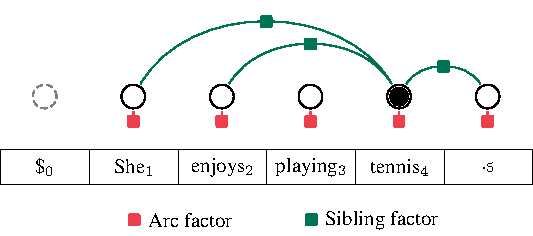
\includegraphics[scale=1]{figures/dep-factors.pdf}
    \caption{依存句法模型的因子图}
    \label{fig:dep-factors}
  \end{subfigure}
  \begin{subfigure}[b]{0.8\textwidth}
    \centering
    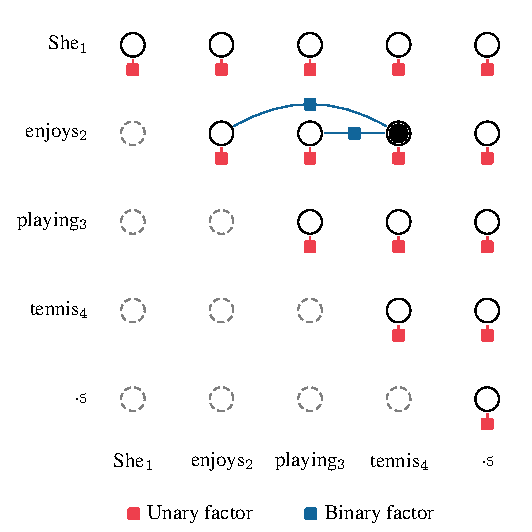
\includegraphics[scale=1]{figures/con-factors.pdf}
    \caption{成分句法模型的因子图}
    \label{fig:con-factors}
  \end{subfigure}
  \caption{一个例句和其依存/成分句法模型对应的因子图,我们在例句上方标出了对应的正确无标签依存句法树和成分句法树,其中成分句法树进行了左二叉化.
    灰色虚线圆圈代表被屏蔽的变量.
    图中标出了所有的一阶(红色)因子,为了简洁起见,对于二阶因子,依存句法图中我们只标出了涉及弧$3\rightarrow 4$的兄弟(绿色)因子,成分句法图中只标出了和组块$(3, 4)$连接的二阶(蓝色)因子.}
  \label{fig:vi-factors}
\end{figure}

在得到分值之后,我们的句法分析方法分为两阶段:1)构建无标签树;2)预测标签.
在第二阶段预测标签的时候,我们以贪婪的方式给依存树的每条弧(见章节~\ref{sub@sec:dep-crf-labeling})或者成分树的每个组块(见章节~\ref{sub@sec:con-crf-model-definition})打上标签.
而在第一阶段构建无标签树时,我们的目的是选择后验概率最大的句法树$\boldsymbol{y} = \arg\max_{\boldsymbol{y}^{\prime}} P(\boldsymbol{y}^{\prime}\mid \boldsymbol{x})$.
通常这样的推断的复杂度较高,以至于无法计算.
在句法分析领域我们可以应用复杂度为$O(n^3)$的Inside算法来进行精确计算,尽管在前面章节我们展示了可以通过批次化以及张量并行计算来降低复杂度,但是仍然十分影响计算效率.
因此在本节我们提出利用基于平均场理论的变分推断法(Mean Field Variational Inference, \textsc{Mfvi})来近似得到后验概率.
\textsc{Mfvi}假设句法树$\boldsymbol{y}$每个位置的变量相互独立,因此可以在线性时间内通过迭代的方法得到后验概率的近似值$Q(\boldsymbol{y})$.

关于\textsc{Mfvi}的通用更新公式以及相关推导见附录~\ref{appendix:mfvi-derivation}.
根据依存句法和成分句法任务目标的不同,我们在下面两小节详细阐述了通用公式针对具体任务的特化版本,以及相关的势函数(potential function)和因子图(factor graph)的设计.

\noindent\textbf{基于头选择的变分推断.}
目前广泛使用的一阶局部模型(对应于章节~\ref{cha:dep-crf}的\textsc{Loc}方法,这里我们称为\textsc{Loc}$_{dep}$)在训练的时候采用了头选择(head selection)训练目标,要求句子中除了根结点之外的每个词有且仅有一个头.
和\citep{wang-tu-2020-second}一样,我们选择在依存句法对应变分推断方法中引入头选择约束,相应的因子图见图~\ref{fig:dep-factors}..
对于每个位置$j$,我们定义变量取值为$y_j\in \{0,1,\cdots,i\neq j,\cdots,n\}$,代表词$w_j$的可能的头索引.

具体地,对于每个变量$y_j$,一阶的势函数定义为
\begin{equation}
  \label{eq:dep-1o-potential}
  \psi_j(y_j)=\exp(s(y_j\rightarrow j))
\end{equation}
$s(y_j\rightarrow j)$是弧$y_j\rightarrow j$对应的分值,由公式~\ref{eq:biaffine}计算得到.

对于两个变量$y_{j}$和$y_{k}$,我们使用和章节~\ref{cha:dep-crf}一致的二阶特征,对应的二阶势函数定义为
\begin{equation}
  \label{eq:2o-dep-potential}
  \psi_{j,k}(y_j,y_k)=\left\{
  \begin{array}{rcl}
    \exp \mathrm{s}(y_j\rightarrow \{k,j\}) &  & {y_j=y_k}   \\
    1                                       &  & {otherwise}
  \end{array}
  \right.
\end{equation}
$s(y_j\rightarrow \{k,j\})$是兄弟子树$y_j\rightarrow \{k,j\}$的分值,由公式~\ref{eq:triaffine}计算得到.
需要注意的是这里的兄弟$k$和二阶TreeCRF不一样,并不需要一定和$j$邻近.

\textsc{Mfvi}迭代式地更新近似分布$Q(\cdot)$,来最小化其与真实分布$P(\cdot)$的KL散度,依存句法模型的迭代更新公式如下\citep{wang-tu-2020-second}:
\begin{equation}
  \label{eq:mfvi-dep}
  Q_{j}^{(t)}(i)\propto \exp\left(s(i\rightarrow j) +\sum_{k\neq i,j} Q_{k}^{(t-1)}(i)\cdot s(i\rightarrow {k,j}) \right)
\end{equation}
后验概率$Q_j^{(0)}(i)$初始化为一阶势函数$\psi_j(i)$.
每次迭代时,我们都会将$Q_j^{(0)}(\cdot)$的值在所有可能的头取值上进行归一化.

\noindent\textbf{基于二分类的变分推断.}
我们的成分句法分析模型采用了\citep{gaddy-etal-2018-whats}的方法作为基线方法,称为\textsc{Loc}$_{con}$.
具体来说,模型对短语树所有可能的位置进行一个简单的二分类,预测该位置是否是一个区块.
\citep{dozat-manning-2018-simpler,wang-etal-2019-second}在语义依存分析中应用了这样的训练目标.
\citep{gormley-eisner-2015-structured,naradowsky-etal-2012-grammarless}在成分句法分析中应用了这种方法,并采用循环置信传播(Loopy Belief Propagation, LBP)来近似获得后验概率,并设计了若干种局部和全局因子,比如\textsc{Exactly1}、\textsc{Tree}等.
我们将其引入到了基于\textsc{Mfvi}的成分句法分析中,但是简单起见仅仅采用了一个一阶因子和一个二阶因子,对应的因子图见图~\ref{fig:con-factors}.
我们考虑将引入更多因子约束的近似算法留待作为未来工作.


具体地,每个位置$ij$的可能的变量取值$y_{ij}\in \{0,1\}$. 对于单个变量$y_{ij}$,一阶的势函数定义为
\begin{equation}
  \label{eq:con-1o-potential}
  \psi_{ij}(y_{ij})=\left\{
  \begin{array}{rcl}
    \exp\left(\mathrm{s}(i,j)\right) &  & {y_{ij}=1}  \\
    1                                &  & {otherwise}
  \end{array}
  \right.
\end{equation}
$s(i,j)$是区块$(i,j)$的分值,由公式~\ref{eq:con-biaffine}计算得到,这里我们要求$i<j$.

给定两个变量$y_{ij}$和$y_{lk}$,我们考虑使用和章节~\ref{cha:con-crf}一致的二阶兄弟特征,因此二阶的势函数定义为
\begin{equation}
  \label{eq:2o-con-potential}
  \psi_{ij,lk}(y_{ij},y_{lk})=\left\{
  \begin{array}{rcl}
    \exp\left(\mathrm{s}(i,k,j)\right) &  & {i=l}       \\
    1                                  &  & {otherwise}
  \end{array}
  \right.
\end{equation}
$s(i,k,j)$可以视为$(i,j)$和$(i,k)$都作为组块时,组成的子树的分值,由公式~\ref{eq:con-triaffine}计算得到,这里$k$的位置不受动态规划算法的约束,并不要求一定位于$(i,j)$之间,即有$i<j,k$.

成分句法模型的\textsc{Mfvi}迭代更新公式如下:
\begin{equation}
  \label{eq:mfvi-con}
  \begin{array}{l}
    Q_{ij}^{(t)}(0)\propto 1 \\
    Q_{ij}^{(t)}(1)\propto \exp\left(s(i,j) +\sum_{k\neq i,j} Q_{ik}^{(t-1)}(1)\cdot s(i,k,j) \right)
  \end{array}
\end{equation}
后验概率$Q_{ij}^{(0)}(y_{ij})$初始化为一阶势函数$\psi_{ij}(y_{ij})$.
每次迭代时,我们将$Q_{ij}^{(0)}(\cdot)$在取值$\{0,1\}$上进行归一化.


\subsection{训练}

我们的训练损失函数分为两部分,分别是无标签树的损失和对应标签的损失.
给定所有正确标签,我们的目标是最大化树上每个标签的概率,和前面的章节一致,我们采用了弧/区块级别的标准交叉熵损失函数.
给定输入句子$\boldsymbol{x}$和对应正确的无标签句法树$\boldsymbol{y}^{\ast}$,我们的目标是最大化句法树的概率$P(\boldsymbol{y}^{\ast}\mid\boldsymbol{x})$.
由于\textsc{Mfvi}将概率在每个变量上分解,得到近似概率$Q(\boldsymbol{y}^{\ast})$,因此训练目标等价于最大化每个变量的后验概率.

对于每个句子,依存句法分析相应无标签句法树的目标函数为
\begin{equation}
  \label{eq:dep-vi-arc-loss}
  L_{dep}^{arc}=-\sum_{j\neq 0}\log Q_j(\boldsymbol{y}^{\ast}_j)
\end{equation}

成分句法的无标签句法树的目标函数为
\begin{equation}
  \label{eq:con-vi-bracket-loss}
  L_{con}^{bracket}=-\sum_{i<j}\log Q_{ij}(\boldsymbol{y}^{\ast}_{ij})
\end{equation}
对于最终的目标函数,我们新引入了一个参数$\lambda$用于平衡无标签句法树以及标签的损失,相应的最终训练目标为
\begin{equation}
  \label{eq:con-vi-loss}
  L_{con}=\lambda L_{con}^{label}+(1-\lambda)L_{con}^{bracket}
\end{equation}

\subsection{解码}
在\textsc{Mfvi}模型中,解码时我们直接应用了MBR解码.
我们直接用\textsc{Mfvi}近似得到的后验概率作为解码算法的输入.
依存句法中,我们将由公式~\ref{eq:mfvi-dep}得到的概率$Q_i(\cdot)$作为输入,并利用了Eisner算法来解码,加速时采用了算法~\ref{alg:eisner-2o}的批次化技术.
成分句法中,我们将由公式~\ref{eq:mfvi-con}得到的概率$Q_{ij}(\cdot)$作为输入,并利用了和章节~\ref{cha:con-crf}一样的类CKY算法来解码,采用了算法~\ref{alg:inside}的批次化技术来加速.


\section{实验}\label{sec:vi-exp}

\noindent\textbf{数据.}
为了方面和章节~\ref{cha:dep-crf}提出的精确推断的高阶模型进行比较,我们主要在英文的PTB和中文的CNLL09上进行了依存句法的实验.
同样的,我们在英文的PTB,中文的CTB51以及CTB7进行了成分句法分析实验.
实验数据的详细设置在章节~\ref{cha:dep-crf}和章节~\ref{cha:con-crf}有详细的设置,这里简洁起见不再重复.

\noindent\textbf{评价.}
在依存句法分析上,我们主要采用了有标签和无标签附着分值(UAS/LAS)作为评价指标,英文PTB的标点被忽略.
在成分句法分析上,我们采用了惯用的区块级别的准确率、召回率和$\mathrm{F}_1$值(P/R/$\mathrm{F}_1$)的指标,由标准工具\texttt{EVALB}来得到.
成分句法树在训练和评价时采用的预处理和后处理行为我们保持和章节~\ref{cha:con-crf}一致.

\noindent\textbf{参数设置.}
我们保持两种句法分析模型的编码器和训练方法与前面的章节基本一致.
对于二阶模型,我们设置依存句法分析中使用的兄弟特征以及成分句法分析使用的二阶特征的MLP层输出维度为100.
我们设置变分推断的迭代次数统一为3次.
对于在成分句法分析中的用于平衡标签和无标签树的训练损失的参数$\lambda$,我们设置$\lambda$为0.1.

\begin{table}[tb!]
  \centering
  \caption{依存句法分析模型在PTB和CoNLL09的Test数据上不同推断算法的结果.}
  \begin{tabular}{lcccc}
    \toprule
                   & \multicolumn{2}{c}{PTB} & \multicolumn{2}{c}{CoNLL09}                                   \\
                   & UAS                     & LAS                         & UAS            & LAS            \\[2pt]
    \midrule
    \\[-15pt]
    \textsc{Loc}   & 96.08                   & 94.47                       & 89.15          & 85.98          \\
    \textsc{Crf}   & 96.02                   & 94.33                       & 89.28          & 86.18          \\
    \textsc{Mfvi}  & \textbf{96.11}          & \textbf{94.49}              & 89.35          & 86.25          \\
    \textsc{Crf2o} & \textbf{96.11}          & 94.46                       & \textbf{89.63} & \textbf{86.52} \\
    \multicolumn{5}{c}{+BERT}                                                                                \\[3pt]
    \textsc{Loc}   &                                                                                         \\
    \textsc{Crf}   &                                                                                         \\
    \textsc{Mfvi}  &                                                                                         \\
    \textsc{Crf2o} &                                                                                         \\
    \bottomrule
  \end{tabular}
  \label{table:vi-dep-test}
\end{table}




\subsection{结果}
表格~\ref{table:vi-dep-test}和表格~\ref{table:vi-con-test}分别给出了我们尝试的多种推断算法在依存句法和成分句法分析上的比较性实验结果.
和章节~\ref{cha:dep-crf}以及章节~\ref{cha:con-crf}一样,我们在所有模型中都使用了预训练词向量作为输入.
英文数据我们统一使用了100维的Glove词向量,中文数据则使用了word2vec在Giga数据上训练的100维词向.
我们还汇报了BERT的结果,对于英文数据,我们使用了24层1024维的\texttt{bert-large-cased}作为双向LSTM的输入,并在训练时固定参数.
中文数据我们则使用了12层768维的\texttt{bert-base-chinese}.

可以看到在依存句法的结果上(表格~\ref{table:vi-dep-test}),由于英文PTB的结果非常高,因此这四种推断方法的结果都十分接近,\textsc{MFVI}方法超越了\textsc{Loc},达到了最好的性能.
中文CoNLL09上,精确推断的\textsc{Crf2o}仍然是最好的,但是\textsc{MFVI}超越了\textsc{Crf}达到了86.25的LAS.
在两种语言上,\textsc{MFVI}都一致超越了没有全局结构约束的\textsc{Loc}方法.
这验证了在近似推断的\textsc{MFVI}方法上应用二阶结构约束的有效性.

在成分句法分析上(表格~\ref{table:vi-con-test}),中英文三个数据的结果中,无论是一阶\textsc{Crf}还是二阶\textsc{Crf2o},精确推断算法都仍然是表现最好的.
然而\textsc{Mfvi}都达到了和一阶\textsc{Crf}十分相近的性能.
并且,\textsc{Mfvi}一致超越了基于二分类学习的\textsc{Loc}模型,在PTB、CTB51和CTB7上分别提升了0.11、0.52和0.35.

当使用BERT之后,上述的几种推断算法在结果上没有显著差异.
依存句法上,PTB中\textsc{Mfvi}表现最好,LAS为95.37,达到或超越了当前的最佳性能\citep{zhou-zhao-2019-head,wang-tu-2020-second},CoNLL09上人仍然\textsc{Crf2o}最佳,但是\textsc{Mfvi}的差距十分微弱.
成分句法中在PTB和CTB51这两个数据上,\textsc{Mfvi}的表现都是最好的,分别达到95.71和92.56的$\mathrm{F}_1$值,高于当前最佳的模型\cite{kitaev-etal-2019-multilingual}.
在CTB7上表现最好的仍是\textsc{Crf2o},$\mathrm{F}_1$值为91.62,而\textsc{Mfvi}的差距不到0.1.
然而,基于\textsc{Mfvi}方法的近似推断在解析效率上有很大的优越性(见章节~\ref{sub@sec:vi-speed}的复杂度分析).

\begin{table}[tb!]
  \centering
  \caption{成分句法分析模型在英文PTB、中文CTB5.1和CTB7的Test数据上不同推断算法的结果.}
  \begin{tabular}{lccccccccc}
    \toprule
                   & \multicolumn{3}{c}{PTB} & \multicolumn{3}{c}{CTB51} & \multicolumn{3}{c}{CTB7}                                                                                                       \\
                   & $\mathrm{P}$            & $\mathrm{R}$              & $\mathrm{F}_1$           & $\mathrm{P}$   & $\mathrm{R}$   & $\mathrm{F}_1$ & $\mathrm{P}$   & $\mathrm{R}$   & $\mathrm{F}_1$ \\[2pt]
    \midrule
    \\[-15pt]
    \textsc{Loc}   & 94.16                   & 93.85                     & 94.01                    & 89.39          & 89.16          & 89.28          & 88.54          & 87.96          & 88.25          \\
    \textsc{Crf}   & 94.23                   & 94.02                     & 94.12                    & 89.71          & \textbf{89.89} & 89.80          & 88.84          & 88.36          & 88.60          \\
    \textsc{Mfvi}  & 94.11                   & 93.96                     & 94.04                    & 89.82          & 89.79          & \textbf{89.81} & 88.71          & 88.16          & 88.43          \\
    \textsc{Crf2o} & \textbf{94.29}          & \textbf{94.15}            & \textbf{94.22}           & \textbf{89.97} & 89.47          & 89.72          & \textbf{88.95} & \textbf{88.56} & \textbf{88.76} \\
    \multicolumn{10}{c}{+BERT}                                                                                                                                                                            \\[3pt]
    \textsc{Loc}   & 95.70                   & 95.43                     & 95.57                    & 92.47          & 92.09          & 92.28          & 91.90          & 91.24          & 91.57          \\
    \textsc{Crf}   & 95.85                   & 95.53                     & 95.69                    & 92.51          & 92.04          & 92.27          & 91.73          & \textbf{91.38} & 91.55          \\
    \textsc{Mfvi}  & 95.85                   & \textbf{95.57}            & \textbf{95.71}           & \textbf{92.78} & \textbf{92.35} & \textbf{92.56} & 91.89          & 91.31          & 91.60          \\
    \textsc{Crf2o} & \textbf{95.86}          & 95.47                     & 95.67                    & 92.75          & 92.18          & 92.47          & \textbf{91.93} & 91.31          & \textbf{91.62} \\
    \bottomrule
  \end{tabular}
  \label{table:vi-con-test}
\end{table}



% \subsection{分析}


\subsection{样例学习}

\begin{figure}[tb!]
  \centering
  \begin{subfigure}[b]{0.9\textwidth}
    \centering
    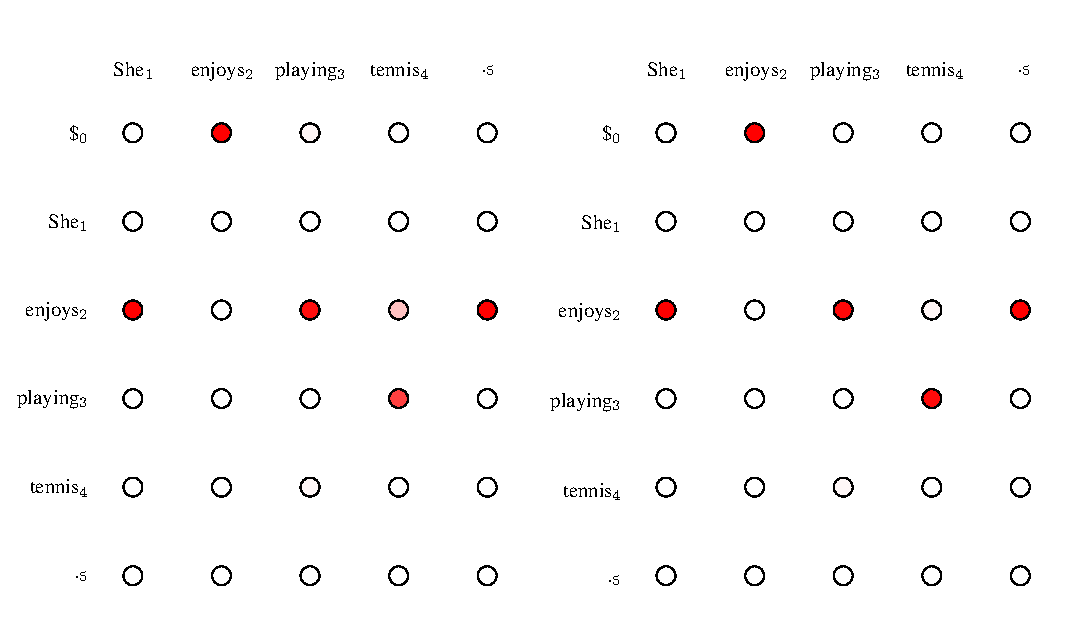
\includegraphics[scale=0.75]{figures/dep-probs.pdf}
    \caption{依存句法树每个位置对应的分值和后验概率}
    \label{fig:dep-probs}
  \end{subfigure}
  \begin{subfigure}[b]{0.9\textwidth}
    \centering
    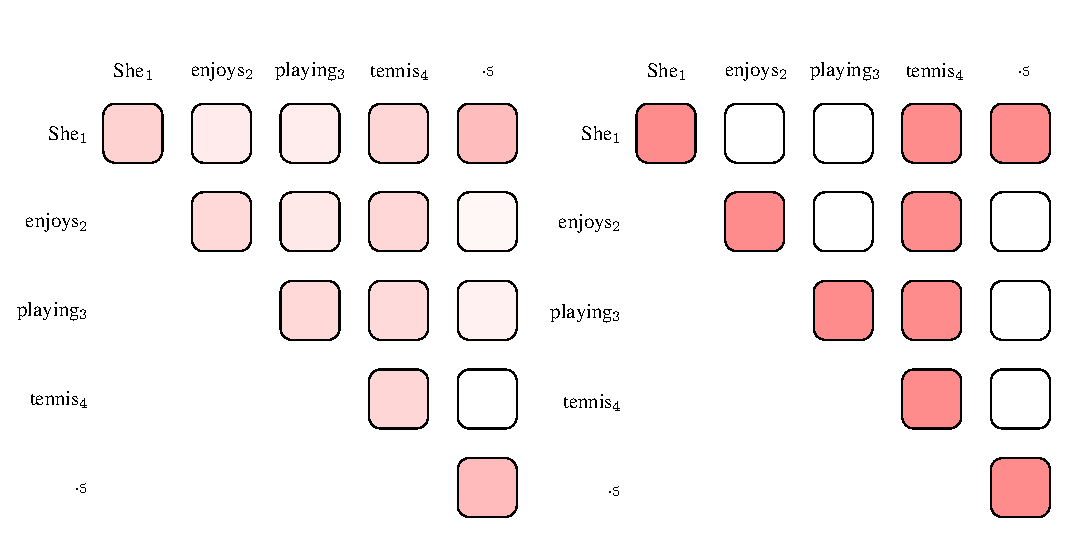
\includegraphics[scale=0.75]{figures/con-probs.pdf}
    \caption{成分句法树每个位置对应的分值和后验概率}
    \label{fig:con-probs}
  \end{subfigure}
  \caption{一个例句对应的依存句法模型和成分句法模型的输出. 左边的图是每个位置的分值(log potential),为了方便显示,我们首先对分值进行了归一化.
    右边的图是变分推断得到的后验概率. 灰色虚线圆圈代表被屏蔽的不合法位置.}

  \label{fig:vi-probs}
\end{figure}

图~\ref{fig:vi-probs}给出了一个例句分别在依存和成分句法模型上的分值(log potentials)与经过\textsc{Mfvi}迭代近似得到的后验概率的热力图对比.
图中颜色的深浅反应了分值/概率的大小.

左边的图反应的是模型直接输出的分值之间的对比,这对应于一阶模型的输出.
可以看到模型的输出的分值数值相对来说都比较均匀.
由于依存句法模型基于的是头选择的训练目标,可以看到图中的每一列都有一个极值存在,比如词$She_i$对应的列中,颜色最深(分值最高)的位置为词$enjoys_2$,这对应了句法树中的弧$enjoys_2\rightarrow She_1$.
成分句法的热力图中,由于采用了二分类的目标,因此颜色较深的位置表示更可能成为一个区块.
然而由于没有类似于依存句法的头约束,直接通过对每个位置$\arg\max$得到的所有区块可能无法组成一棵合法的句法树,因此我们仍需要CKY算法来获得全局最优的合法句法树.

当我们利用\textsc{Mfvi}算法,得到的近似后验概率的热力图如右边图所示.
可以看到,在进一步考虑了二阶特征的分值并聚合到每个变量位置之后,后验概率的置信度远远高于分值.
对于依存句法而言,每个词都有一个最可能的头,并且概率几乎为1,对应于热力图中每列仅有一个红色结点.
对于成分句法而言,如果对图中每个位置的后验概率取$\arg\max$得到可能的区块,每个区块的概率同样近似为1,并且对于图中的例句而言,这种贪婪解码得到的句法树可以直接组成一棵合法的短语结构树,例如,红色结点$(She_1,tennis_4)$和$(playing_3,tennis_4)$对应了例句正确的无标签树左二叉化之后的两个区块.
这显示了\textsc{Mfvi}在引入二阶结构打分之后,对于模型结构预测更强大的约束作用.


\subsection{速度和时间复杂度比较}
\label{sub@sec:vi-speed}
\begin{table}[tb!]
  \centering
  \caption{依存句法和成分句法使用不同推断算法的时间复杂度,以及相应的在PTB的Test数据上的解析时间的比较.
    依存句法统一使用了Eisner算法解码,成分句法统一使用了CKY算法解码}
  \begin{tabular}{llcccr}
    \toprule
     & \multirow{2}{*}{Inference} & \multicolumn{2}{c}{Complexity} & \multirow{2}{*}{Decoding Alg.} & \multirow{2}{*}{Sents/sec}                 \\
     &                            & CPU                            & GPU                            &                            &               \\[2pt]
    \midrule
    \multirow{3}{*}{Dependency}
    % & \textsc{Loc}               & $O(n)$                         & $O(1)$                         & Eisner                     & 990           \\
     & \textsc{Crf}               & $O(n^3)$                       & $O(n^2)$                       & Eisner                     & 653           \\
     & \textsc{Crf2o}             & $O(n^3)$                       & $O(n^2)$                       & Eisner                     & 431           \\
     & \textsc{Mfvi}              & $O(n^3)$                       & $O(n)$                         & Eisner                     & \textbf{1126} \\
    \midrule
    \multirow{3}{*}{Constituency}
    % & \textsc{Loc}               & $O(n)$                         & $O(1)$                         & CKY                        & 990           \\
     & \textsc{Crf}               & $O(n^3)$                       & $O(n^2)$                       & CKY                        & 743           \\
     & \textsc{Crf2o}             & $O(n^3)$                       & $O(n^2)$                       & CKY                        & 598           \\
     & \textsc{Mfvi}              & $O(n^3)$                       & $O(n)$                         & CKY                        & \textbf{905}  \\

    \bottomrule
  \end{tabular}
  \label{table:vi-speed}
\end{table}
表~\ref{table:vi-speed}给出了\textsc{Mfvi}和前面章节提及的精确推断模型的速度和复杂度的比较.
为了统一比较,所有的设置下都应用了MBR解码,并且每个任务都用了相同的解码算法.
可以看到,无论是依存句法还是成分句法模型,他们相应的\textsc{Mfvi}在CPU上每一次迭代都需要$O(n^3)$的复杂度,这和精确推断的2阶Inside算法的复杂度相当.
而当利用GPU进行并行计算时,\textsc{Mfvi}每个位置的变量仅需要一次遍历来收集其他位置的信息\footnote{尽管现代的CUDA技术可以通过二叉树等数据结构让并行化的归约操作,例如$\mathrm{sum}$、$\mathrm{min}$和$\mathrm{max}$等,缩减到$O(\log n)$复杂度的时间\citep{wang-etal-2020-ain},但是这里我们统一假设归约操作的复杂度为$O(n)$.},因此GPU上的算法复杂度为$O(n)$,大大快于精确推断所需要的$O(n^2)$复杂度.

从表中可以看到,利用\textsc{Mfvi}的依存句法在PTB的Test数据的解析速度为1126句/秒,是精确推断的二阶\textsc{Crf2o}(431)的近三倍快,同样也大大快于一阶\textsc{Crf}的653句/秒.
成分句法的\textsc{Mfvi}模型的解析速度大约为905句/秒,同样显著快于一阶\textsc{Crf}的743句/秒和二阶\textsc{Crf2o}的598句/秒.

\section{本章小结}

在本章我们将包含二阶特征的\textsc{Mfvi}方法方法引入到了依存句法和成分句法分析中.
根据两种句法分析的特点,在依存句法分析上,我们参考\citep{wang-tu-2020-second}实现了一个包含头选择约束的\textsc{Mfvi}方法,在成分句法分析上,我们引入了一个基于二分类学习目标的\textsc{Mfvi}方法.
在这两个任务的中英文个五个数据集上的结果表明,\textsc{Mfvi}方法均超越了基于局部学习的\textsc{Loc}方法,并达到和精确推断的二阶\textsc{Crf2o}方法可比较的性能.
此外\textsc{Mfvi}方法相比于精确推断的解析速度大大加快.
在加入BERT之后,基于\textsc{Mfvi}方法的近似推断模型在所有的数据集上都达到或者接近了当前最佳的模型.
\chapter{总结与展望}

\section{总结}
得益于深度学习技术的迅速发展,以及神经网络模型的强大建模能力,近年来句法分析领域得到了长足的进步。
\citet{dozat-etal-2017-biaffine}提出的依存句法分析器Biaffine Parser作为当前最流行的句法分析器,代表了这样一个发展趋势:采用一个强大的编码器,结合一个简单的训练目标。
本文将Biaffine Parser作为依存句法和成分句法分析两个任务的骨干架构,探索了进一步提升句法分析模型的途径。

首先,与现有方法采用的局部损失函数或者Max Margin训练方法不同,本文采用了TreeCRF作为主要的推断方法,在训练时寻求最大化句法树的概率。
一方面TreeCRF考虑到了全局树约束,带来了更好的性能。
另一方面,TreeCRF可以显式获得树和子树的概率,对于下游任务而言更加有用。
为了解决TreeCRF带来的低效问题,本文分别采用了:1)批次化Inside算法;2)高效的反向传播机制代替Outside算法;这两项技术来加速。

其次,考虑到在前人方法中采用高阶特征能够带来显著的提升。
本文在一阶模型的基础上提出了一个二阶TreeCRF的扩展,并采用了一个新颖的Triaffine结构来为二阶子树打分。
在两种句法分析任务上的结果表明,二阶TreeCRF都明显超越了一阶基于局部训练目标的模型。

二阶TreeCRF进一步增加了推断算法的复杂度,因此本文还提出利用基于平均场变分推断的近似算法代替二阶TreeCRF。
变分推断方法和二阶TreeCRF采用了相同的高阶子树特征,但是显著降低了复杂度。
在多个数据集上的结果表明,变分推断方法显著超越了一阶模型的结果,并且速度相比于二阶方法要大大提升。

总的来说,本文的主要内容如下:
\begin{enumerate}
	\item 基于TreeCRF的高阶依存句法分析\\
	      \indent 本文以当前最佳的神经依存句法分析模型Biaffine Parser为基础,提出了一个二阶TreeCRF的扩展。
	      对于二阶子树,本文提出了一个新颖的Triaffine结构来打分。
	      为了解决TreeCRF低效的问题,我们提出对于$O(n^3)$复杂的Inside算法进行批次化,利用GPU并行计算的能力将算法复杂度降低到了$O(n^2)$。
	      此外我们将复杂的Outside过程用基于自动求导机制的高效反向传播。
	      我们的加速方法让二阶模型的解析速度达到400句每秒,相比于传统在CPU上运算的方式有数十倍的提升,并且没有明显慢于一阶模型。
	      我们在13个语言的27个数据集上进行了大量的分析和实验,发现二阶模型带来了显著的准确率提升,并且尤其在全局指标,以及局部标注数据上表现良好。
	\item 基于TreeCRF的高阶成分句法分析\\
	      \indent 本文提出在已有神经网络模型的基础上应用高阶TreeCRF到成分句法分析中。
	      为了解决高复杂度问题,我们采用了和依存句法中一致的加速策略,将训练和解码算法进行了高度批次化,并且用支持自动求导机制的反向传播传播算法代替了复杂的Outside算法,从而显著提升了解析速度。
	      此外,我们提出了简单的两阶段解析方法,比前人的一阶段解析更加高效,并且没有损害性能。
	      为了提升解析效果,我们参考依存句法分析对模型架构进行了修改。
	      我们提出用双仿射打分机制代替前人的minus feature方法,并且发现在双向LSTM编码器中引入的一些诸如Dropout的参数修改可以极大提升解析的性能,达到不输于Transformer的效果。
	      在中英文的三个基准数据集上的实验结果表明,我们提出的一阶和二阶成分句法模型显著超越了前人的方法。
	      速度方面,一阶和二阶模型分别可以解析1,000和598句每秒。
	      在使用BERT之后,我们的模型在大部分数据集上都达到了新的最佳结果。
	\item 基于变分推断的高效句法分析方法\\
	      \indent 考虑到精确推断的TreeCRF方法的高复杂度问题,本文中我们将包含二阶特征的平均场变分推断引入到了依存句法和成分句法分析中,使得算法在GPU上的复杂度从$O(n^2)$降低到了$O(n)$。
	      根据两种句法分析任务的不同学习特性,我们采取了不同的变分推断更新策略,在依存句法分析上我们采取了一个包含头选择约束的更新方法,在成分句法分析上我们则引入了一个基于二分类学习目标的更新方法。
	      我们在中英文共五个数据集上做了实验,结果表明我们的方法显著超越了采用局部学习目标的方法,并达到了和精确推断的二阶TreeCRF方法可比较的性能。
	      在使用BERT之后,变分推断方法在所有数据上都达到或接近了现有模型的最佳水平。
\end{enumerate}

\section{未来展望}
本文在依存句法和成分句法分析两个任务上分别尝试了基于树形随机场的融入高阶特征的结构化学习方法,让句法分析模型达到了新的最佳水平。
本文还尝试了应用基于变分推断的近似推断算法,显著降低了高阶TreeCRF的复杂度,大大提升了句法分析速度。
未来,本文打算基于已有成果从一下几个方面继续探索:
\begin{enumerate}
	\item 本文的句法分析模型主要采用了3层双向LSTM作为编码器。
	      考虑到Transformer的迅速发展,以及BERT预训练语言模型的强大作用,未来我们将尝试利用Transformer替换已有编码器,探讨自注意力机制的效果,以及语言模型不同的利用方式,例如特征集成和微调对模型性能的影响。
	\item 本文中为了方便起见我们只采用了一种高阶特征,例如依存模型中我们只采用了邻接兄弟特征,成分模型中采用了区块分割点特征。
	      在未来我们将尝试更多的特征设计,探讨他们对模型效果的影响。
	\item 在本文中我们只尝试了基于平均场变分推断的近似推断算法。
	      然而,仍然有其他的近似算法在NLP社区有广泛的应用,例如循环置信传播、对偶分解、整数线性规划等等。
	      在未来我们打算尝试更多近似算法,并对他们做一些经验性比较。
\end{enumerate}


% % 参考文献,4或者小4楷体
% !Mode:: "TeX:UTF-8"
%\cleardoublepage

\addcontentsline{toc}{chapter}{参考文献}
% \nocite{*}
\begin{kai}
    \bibliography{thesis}
\end{kai}
% \cleardoublepage


% % 附录,4或者小4楷体
\appendix
\chapter{关于Outside算法以及反向传播机制等价性的推导}

\section{Outside算法与反向传播机制的等价性证明}\label{sec:outside-backprop}
我们可以直接用$\log Z(\boldsymbol{x})$(partition term)对每个位置的分值$\mathrm{s}(i, j)$(log potential)求偏导
\begin{equation}
  \label{eq:partial-derivative}
  \begin{split}
    \frac{\partial \log Z}{\partial \mathrm{s}(i, j)} & = \frac{\partial \log Z}{\partial Z} \cdot \frac{\partial Z}{\partial \mathrm{s}(i, j)}\\
    & =\frac{1}{Z} \cdot \frac{\partial \sum_{\boldsymbol{y}} \exp \left(\mathrm{s}(\boldsymbol{x}, \boldsymbol{y}) \right)}{\partial \mathrm{s}(i, j)}\\
    & =\frac{1}{Z} \cdot \frac{\partial \sum_{\boldsymbol{y}:(i,j) \in \boldsymbol{{y}}} \exp \left(\mathrm{s}(\boldsymbol{x}, \boldsymbol{y}) \right)}{\partial \mathrm{s}(i, j)}\\
    & =\frac{1}{Z} \cdot \frac{\sum_{\boldsymbol{y}:(i,j) \in \boldsymbol{{y}}} \exp \left( \sum_{(i^{\prime}, j^{\prime}) \in \boldsymbol{y}\setminus (i,j)} \mathrm{s}(i^{\prime}, j^{\prime}) \right)\cdot \partial \exp(\mathrm{s}(i, j))}{\partial \mathrm{s}(i, j)}\\
    & =\sum_{\boldsymbol{y}:(i,j) \in \boldsymbol{{y}}} \frac{\exp \left( \sum_{(i^{\prime}, j^{\prime}) \in \boldsymbol{y}\setminus (i,j)} \mathrm{s}(i^{\prime}, j^{\prime})\right)\cdot \exp(\mathrm{s}(i,j))}{Z}\\
    &= \sum_{\boldsymbol{y}:(i,j) \in \boldsymbol{{y}}} p(\boldsymbol{y}\mid\boldsymbol{x})\\
  \end{split}
\end{equation}
因此偏导数等价于所有包含$(i,j)$的弧的句法树的概率之和,这正是边缘概率$p(i \rightarrow j\mid\boldsymbol{x})$的定义.

\noindent$\blacksquare$


\section{MBR解码}\label{sec:mbr-decoding}
大体上讲,解码过程是将一个模型输出的概率分布转化为对应的系统输出.
给定输入$\boldsymbol{x}$,理想情况下一个解码器将选择一个$\boldsymbol{y}$,使得$\ell(\boldsymbol{y},\boldsymbol{y}^{\ast})$最小化,其中$\ell(\boldsymbol{y},\boldsymbol{y}^{\ast})$称为代价函数,衡量$\boldsymbol{y}$与真实分配$\boldsymbol{y}^{\ast}$的差异性.
由于通常情况下解码时不存在正确答案,因此我们转而用正确答案的所有可能取值$\boldsymbol{y}^{\prime}$的平均来代替
\begin{equation}
  \label{eq:mbr}
  \boldsymbol{y}= \arg\min_{\boldsymbol{y}}\sum_{\boldsymbol{y}^{\prime}}p(\boldsymbol{y}^{\prime}\mid\boldsymbol{x})\cdot\ell(\boldsymbol{y},\boldsymbol{y}^{\prime})
\end{equation}
上述正是\textbf{最小贝叶斯风险}(Minimum Bayesian Risk, MBR)的内涵:给定输入$\boldsymbol{x}$及对应的后验分布,选择$\boldsymbol{y}$,使得\textit{期望}代价(即风险,\textit{Risk})最小化\citep{stoyanov-eisner-2012-minimum}.

对句法分析,或其他结构化预测任务而言,通常我们采用的是最大后验概率(Maximum \textit{A Posteriori}, MAP)解码,即寻求一个使得后验概率最大化的答案.
这是MBR解码的一个特例,而对应的代价函数$\ell^{MAP}(\cdot)$为一个简单的0-1指示函数,判断$\boldsymbol{y}$与$\boldsymbol{y}^{\prime}$是否一致
\begin{equation}
  \ell^{MAP}(\boldsymbol{y},\boldsymbol{y}^{\prime}) = \mathbbm{1}(\boldsymbol{y}\neq\boldsymbol{y}^{\prime})
\end{equation}
代入到公式~\ref{eq:mbr}得到
\begin{equation}
  \label{eq:map}
  \begin{split}
    \boldsymbol{y}^{MAP}&= \arg\min_{\boldsymbol{y}}\sum_{\boldsymbol{y}^{\prime}}p(\boldsymbol{y}^{\prime}\mid\boldsymbol{x})\cdot\ell^{MAP}(\boldsymbol{y},\boldsymbol{y}^{\prime})\\
    &=\arg\min_{\boldsymbol{y}}\sum_{\boldsymbol{y}^{\prime}}p(\boldsymbol{y}^{\prime}\mid\boldsymbol{x})\cdot\mathbbm{1}(\boldsymbol{y}\neq\boldsymbol{y}^{\prime})\\
    &=\arg\min_{\boldsymbol{y}} 1-p(\boldsymbol{y}\mid\boldsymbol{x})\\
    &=\arg\max_{\boldsymbol{y}}p(\boldsymbol{y}\mid\boldsymbol{x})
  \end{split}
\end{equation}
上式与MAP解码的选择概率最大的$\boldsymbol{y}$的目标等价.

以基于弧分解假设的一阶句法分析模型为例,式~\ref{eq:map}的MAP解码进一步写为
\begin{equation}
  \label{eq:map-dep}
  \begin{split}
    \boldsymbol{y}^{MAP}&=\arg\max_{\boldsymbol{y}}p(\boldsymbol{y}\mid\boldsymbol{x})\\
    &=\arg\max_{\boldsymbol{y}}\frac{\sum_{(i,j)\in \boldsymbol{y}}\mathrm{s}(i,j)}{Z(\boldsymbol{x})\equiv \sum_{\boldsymbol{y}^{\prime}}\sum_{(i^{\prime},j^{\prime})\in \boldsymbol{y}^{\prime}}\mathrm{s}(i^{\prime},j^{\prime})}\\
    &=\arg\max_{\boldsymbol{y}}\sum_{(i,j)\in \boldsymbol{y}}\mathrm{s}(i,j)
  \end{split}
\end{equation}
去掉共同的分母,分子为对应句法树的分值,上式的含义是获取分值最大的句法树,这个目标可以通过常见的一些解码算法(如Eisner,MST等)达到.

而对于MBR解码,我们定义代价函数为在每条弧上的指示函数,
\begin{equation}
  \ell^{MBR}(\boldsymbol{y},\boldsymbol{y}^{\prime}) = \sum_{(i,j)\in\boldsymbol{y},(i,j^{\prime})\in\boldsymbol{y}^{\prime}}\mathbbm{1}(j\neq j^{\prime})
\end{equation}
代入到公式~\ref{eq:mbr}得到
\begin{equation}
  \label{eq:mbr-dep}
  \begin{split}
    \boldsymbol{y}^{MBR}&= \arg\min_{\boldsymbol{y}}\sum_{\boldsymbol{y}^{\prime}}p(\boldsymbol{y}^{\prime}\mid\boldsymbol{x})\cdot\ell^{MBR}(\boldsymbol{y},\boldsymbol{y}^{\prime})\\
    &=\arg\min_{\boldsymbol{y}}\sum_{\boldsymbol{y}^{\prime}}p(\boldsymbol{y}^{\prime}\mid\boldsymbol{x})\cdot\sum_{(i,j)\in\boldsymbol{y},(i,j^{\prime})\in\boldsymbol{y}^{\prime}}\mathbbm{1}(j\neq j^{\prime})\\
    &=\arg\min_{\boldsymbol{y}}\sum_{(i,j)\in\boldsymbol{y},(i,j^{\prime})\in\boldsymbol{y}^{\prime}}\sum_{\boldsymbol{y}^{\prime}}p(\boldsymbol{y}^{\prime}\mid\boldsymbol{x})\cdot\mathbbm{1}(j\neq j^{\prime})\\
    &=\arg\min_{\boldsymbol{y}}\sum_{(i,j)\in\boldsymbol{y}}\sum_{\boldsymbol{y}^{\prime}:(i,j)\notin \boldsymbol{y}^{\prime}}p(\boldsymbol{y}^{\prime}\mid\boldsymbol{x})\\
    &=\arg\min_{\boldsymbol{y}}\sum_{(i,j)\in\boldsymbol{y}}\left(1-\sum_{\boldsymbol{y}^{\prime}:(i,j)\in \boldsymbol{y}^{\prime}}p(\boldsymbol{y}^{\prime}\mid\boldsymbol{x})\right)\\
    &=\arg\max_{\boldsymbol{y}}\sum_{(i,j)\in\boldsymbol{y}}\sum_{\boldsymbol{y}^{\prime}:(i,j)\in \boldsymbol{y}^{\prime}}p(\boldsymbol{y}^{\prime}\mid\boldsymbol{x})\\
    &=\arg\max_{\boldsymbol{y}}\sum_{(i,j)\in\boldsymbol{y}}p(i\rightarrow j\mid\boldsymbol{x})
  \end{split}
\end{equation}
式~\ref{eq:mbr-dep}和式~\ref{eq:map-dep}的唯一区别在于要求和的项是边缘概率而非分值.
因此,在一阶依存句法分析的场景下,MBR解码只需要给定弧的边缘概率,然后直接应用和MAP解码一样的解码算法即可\citep{smith-smith-2007-probabilistic, smith-2011-linguistic}.

\noindent$\blacksquare$


\chapter{用于结构化预测的平均场变分推断的推导}
\label{appendix:mfvi-derivation}
对于一般的结构化任务而言,我们需要得到后验分布$P(\boldsymbol{y}\mid\boldsymbol{x})$。
我们可以将输出$\boldsymbol{y}$按照对应的因子图分解为若干个因子的集合 \citep{sutton-etal-2012-crf},相应的$P(\boldsymbol{y}\mid\boldsymbol{x})$定义为\footnote{后面方便起见我们省略输入$\boldsymbol{x}$的标记}
\begin{equation}\label{eq:posterior}
	P(\boldsymbol{y}\mid\boldsymbol{x}) =\frac{\prod_{\alpha} \psi_{\alpha}(y_{\alpha})}{Z(\boldsymbol{x})\equiv\sum_{\boldsymbol{y}^{\prime}}\prod_{\alpha} \psi_{\alpha}(y^{\prime}_{\alpha})}
\end{equation}
其中$Z$为配分项,$\psi_{\alpha}(\cdot)$为因子$\alpha$的势函数,我们定义未归一化的分布$\tilde{P}(\boldsymbol{y})=\prod_{\alpha} \psi_{\alpha}(y_{\alpha})$。

变分推断建模一个近似分布$Q(\boldsymbol{y})$,并最小化其与真实分布的KL散度(Kullback–Leibler Divergence)
\begin{equation}
	\begin{split}
		Q^{\ast}(\boldsymbol{y})
		&=\arg\min_{Q} KL(Q\|P)\\
		&=\arg\min_{Q} E_{Q}\left[\log\frac{Q(\boldsymbol{y})}{P(\boldsymbol{y})}\right]\\
		&=\arg\min_{Q} E_{Q}\left[\log Q(\boldsymbol{y})\right] - E_{Q}\left[\log P(\boldsymbol{y})\right]\\
		&=\arg\min_{Q} \log Z-\underbrace{\left(E_{Q}\left[\log \tilde{P}(\boldsymbol{y})\right]-E_{Q}\left[\log Q(\boldsymbol{y})\right]\right)}_{ELBo}
	\end{split}
\end{equation}
去掉配分项,定义
\begin{equation}
	\mathcal{L}(Q)=ELBo=E_{Q}\left[\log \tilde{P}(\boldsymbol{y})\right]-E_{Q}\left[\log Q(\boldsymbol{y})\right]
\end{equation}
我们将最小化KL散度的目标函数代替为最大化ELBo
\begin{equation}
	\begin{split}
		Q^{\ast}(\boldsymbol{y}) &= \arg\max_{Q}\mathcal{L}(Q)\\
		&= \arg\max_{Q}E_{Q}\left[\log \tilde{P}(\boldsymbol{y})\right]-E_{Q}\left[\log Q(\boldsymbol{y}))\right]
	\end{split}
\end{equation}


Mean Field假设每个变量相互独立,即有$Q(\boldsymbol{y})=\prod_i{Q_i(y_i)}$。
因此上式可应用坐标上升法(Coordinate Ascent),每次迭代优化一个变量$Q_j(y_j)$,保持其余变量$Q_{-j}(y_{-j})$不变。
对于目标函数
\begin{equation}
	\mathcal{L}(Q)=\underbrace{E_{Q}\left[\log \tilde{P}(\boldsymbol{y})\right]}_{\tcircle{1}}-\underbrace{E_{Q}\left[\log Q(\boldsymbol{y})\right]}_{\tcircle{2}}
\end{equation}
分别有
\begin{equation}
	\begin{split}
		\tcircle{1}&=E_{Q}\left[\log \tilde{P}(\boldsymbol{y})\right]\\
		&=\int_{\boldsymbol{y}}Q(\boldsymbol{y}) \log \tilde{P}(\boldsymbol{y})d\boldsymbol{y}\\
		&=\int_{\boldsymbol{y}}\prod_i{Q_i(y_i)} \log \tilde{P}(\boldsymbol{y})d\boldsymbol{y}\\
		&=\int_{y_j}Q_j(y_j)\left(\int_{y_{-j}}Q_{-j}(y_{-j})\log \tilde{P}(\boldsymbol{y}) dy_{-j}\right) dy_j\\
		&=\int_{y_j}Q_j(y_j)E_{Q_{-j}}\left[\log \tilde{P}(\boldsymbol{y}) \right] dy_j\\
		\tcircle{2}&=E_{Q}\left[\log Q(\boldsymbol{y}))\right]\\
		&=\int_{\boldsymbol{y}}Q(\boldsymbol{y}) \sum_i\log Q_i(y_i) d\boldsymbol{y}\\
		&=\int_{\boldsymbol{y}}\prod_i{Q_i(y_i)} \sum_i\log Q_i(y_i) d\boldsymbol{y}\\
		&=\sum_i\int_{\boldsymbol{y}}Q_i(y_i)Q_{-i}(y_{-i})\log Q_i(y_i) d\boldsymbol{y}\\
		&=\sum_i\int_{y_i}Q_i(y_i)\log Q_i(y_i) dy_i\int_{y_{-i}} {Q_{-i}(y_{-i})}dy_{-i}\\
		&=\sum_i\int_{y_i}Q_i(y_i)\log Q_i(y_i) dy_i\\
		&=\int_{y_j}Q_j(y_j)\log Q_j(y_j) dy_j + \sum_{i\neq j}\int_{y_i}Q_i(y_i)\log Q_i(y_i) dy_i  \\
		&=\int_{y_j}Q_j(y_j)\log Q_j(y_j) dy_j + C
	\end{split}
\end{equation}
$C$代表常数项,因此有
\begin{equation}
	\begin{split}
		\mathcal{L}(Q)&=\tcircle{1}-\tcircle{2}\\
		&=\int_{\boldsymbol{y_j}}Q_j(y_j)\underbrace{E_{Q_{-j}}\left[\log \tilde{P}(\boldsymbol{y}) \right]}_{\log \dot{P}_j(y_j)} dy_j-\int_{y_j}Q_j(y_j)\log Q_j(y_j) dy_j +C\\
		&=\int_{\boldsymbol{y_j}}Q_j(y_j)\log\frac{\dot{P}_j(y_j)}{Q_j(y_j)} dy_j +C\\
		&=-KL\left(Q_j(y_j)\|\dot{P}_j(y_j)\right)+C
	\end{split}
\end{equation}
因此最大化$\mathcal{L}(Q)$即最小化$KL\left(Q_j(y_j)\|\dot{P}_j(y_j)\right)$。
当两个分布相等时KL散度最小,因此相应的更新公式为
\begin{equation}
	\begin{split}
		Q^{\ast}_j(y_j)
		&=\exp\left(E_{Q_{-j}}\left[\log \tilde{P}(\boldsymbol{y}) \right]\right)\\
		&=\exp\left(E_{Q_{-j}}\left[\log \prod_{\alpha}\psi_{\alpha}(y_{\alpha}) \right]\right)\\
		&=\exp\left(\int_{y_{-j}} Q_{-j}(y_{-j})\sum_{\alpha}\log \psi_{\alpha}(y_{\alpha}) dy_{-j}\right)\\
		&=\exp\left(\sum_{\alpha}\int_{y_{-j}} Q_{-j}(y_{-j})\log \psi_{\alpha}(y_{\alpha}) dy_{-j}\right)\\
		&\propto\exp\left(\sum_{\alpha:j\in \mathcal{N}(\alpha)}\int_{y_{-j}} Q_{-j}(y_{-j})\log \psi_{\alpha}(y_{\alpha}) dy_{-j}\right)\\
	\end{split}
\end{equation}
$\mathcal{N}(\alpha)$代表与因子$\alpha$连接的变量,上式中,所有与变量$j$无关的因子对应的积分之和为一个常数项。
继续推导得
\begin{equation}
	\begin{split}
		Q^{\ast}_j(y_j)
		&\propto\exp\left(\sum_{\alpha:j\in \mathcal{N}(\alpha)}\int_{y_{-j}} Q_{-j}(y_{-j})\log \psi_{\alpha}(y_{\alpha}) dy_{-j}\right)\\
		&\propto\exp\left(\sum_{\alpha:j\in \mathcal{N}(\alpha)}\int_{y_{\mathcal{N}(\alpha)-j}} Q_{\mathcal{N}(\alpha)-j}(y_{\mathcal{N}(\alpha)-j})\log \psi_{\alpha}(y_{\alpha}) dy_{\mathcal{N}(\alpha)-j}\int_{y_{-\mathcal{N}(\alpha)}} Q_{-\mathcal{N}(\alpha)}(y_{-\mathcal{N}(\alpha)}) dy_{-\mathcal{N}(\alpha)}\right)\\
		&\propto\exp\left(\sum_{\alpha:j\in \mathcal{N}(\alpha)}\int_{y_{\mathcal{N}(\alpha)-j}} Q_{\mathcal{N}(\alpha)-j}(y_{\mathcal{N}(\alpha)-j})\log \psi_{\alpha}(y_{\alpha}) dy_{\mathcal{N}(\alpha)-j}\right)\\
		&\propto\exp\left(\sum_{\alpha:j\in \mathcal{N}(\alpha)}E_{Q_{\mathcal{N}(\alpha)-j}}\log \psi_{\alpha}(y_{\alpha})\right)\\
	\end{split}
\end{equation}
因此,更新公式为
\begin{equation}
	Q^{\ast}_j(y_j)\propto\exp\left(\sum_{\alpha:j\in \mathcal{N}(\alpha)}E_{Q_{\mathcal{N}(\alpha)-j}}\log \psi_{\alpha}(y_{\alpha})\right)
\end{equation}
对于包含高阶因子的模型,我们引入记号$\alpha$和$\beta$分别代表一阶因子和高阶因子。
容易得,相应的更新公式为
\begin{equation}
	Q^{\ast}_j(y_j)\propto\psi_{\alpha}(y_{\alpha})\cdot\exp\left(\sum_{\beta:j\in \mathcal{N}(\beta)}E_{Q_{\mathcal{N}(\beta)-j}}\log \psi_{\beta}(y_{\beta})\right)
\end{equation}
\noindent$\blacksquare$


% 附页标题样式
\backmatter
% 附页
\chapter{攻读学位期间的成果}

\begin{itemize}
	\setlength{\itemsep}{5pt}
	% \setlength{\parsep}{2em}
	
	\item \textbf{\heiti\sihao{论文}}
	      \begin{enumerate}
	      	\setlength{\itemsep}{-\itemsep}  %调整间距
	      	% \usecounter{numcount} % 使用计数器,初始值为0
	      	% \setlength{\leftmargin}{3em} %左边界
	      	% \setlength{\parsep}{-0.5ex} %段落间距
	      	% \setlength{\topsep}{-10ex} %列表到上下文的垂直距离
	      	% \setlength{\itemsep}{0.5ex} %条目间距
	      	% \setlength{\labelsep}{0.3em} %标号和列表项之间的距离,默认0.5em
	      	% \setlength{\itemindent}{1.1em} %标签缩进量
	      	% \setlength{\listparindent}{0em} %段落缩进量
	      	
	      	\item Annual Meeting of the Association for Computational Linguistics (ACL, CCF-A会议). 2020. 一作. 已录用
	      	\item International Joint Conference on Artificial Intelligence (IJCAI, CCF-A会议). 2020. 一作. 已录用
	      	\item Natural Language Processing and Chinese Computing (NLPCC, CCF-C会议). 2020. 共同一作. 已录用
	      	\item International Workshop on Semantic Evaluation (SemEval). 2019. 三作. 已录用
	      	      
	      \end{enumerate}
	      
	\item \textbf{\heiti\sihao{比赛}}
	      \begin{enumerate}
	      	\item *2020语言与智能技术竞赛比赛,第六名.
	      	\item *2019语义分析国际评测比赛,第一名.
	      \end{enumerate}
	      
	\item \textbf{\heiti\sihao{实习}}
	      \begin{enumerate}
	      	\item \textsc{2020/8--2021/2}. 杭州-阿里巴巴-达摩院.
	      \end{enumerate}
	      
\end{itemize}

\chapter{致谢}

养天地正气,法古今完人.
从本科到硕士,转眼间在美丽的苏州大学校园内度过了七年的求学时光.
在这段不算短的人生旅途中,无论是学识上还是生活阅历上我都成长良多.

首先,我要感谢我的导师李正华老师.
李老师永远以饱满的热情和专注的态度面对工作和生活,永远是我以后希望成为一个独立研究者的榜样.

感谢尊敬的张民老师,张老师以高标准要求每一个学生,营造了组内专一浓厚的科研氛围.
此外,张老师敏锐的思维、渊博的知识、平易近人的风格、深深的影响了我,平时的相处让我获益良多.
感谢陈文亮老师,陈老师开朗热情,在学业上也给予了我很多指导.

同样感谢周国栋、朱巧明、李寿山、洪宇和李军辉等苏州大学自然语言处理实验室的所有老师,各位老师严谨的治学态度和进取的专业精神是我的榜样.

感谢同组的夏庆荣师兄、龚晨师姐、李英师姐和张月师姐,各位师兄师姐总是十分热心的解决我生活和研究上遇到的困难.
感谢章波、黄德朋、江心舟师兄,彭雪师姐,在我还是萌新的时候对我的帮助,以及平时对我的关照.
感谢同届的同学蒋炜、陆凯华、吴锟、刘亚慧,大家在一起互相帮助,互相进步.
感谢周厚全、沈嘉钰、李嘉诚、侯洋、李帅克、周仕林、刘泽洋、李扬师弟,还有周明月、杨浩萍师妹,十分珍惜与大家相处的美好时光.
此外,还要感谢实习期间相处的蒋勇师兄以及王新宇同学,特别是感谢蒋勇师兄在我实习期间对我的关照,以及在课题研究上的悉心帮助和指导.

感谢我的父母还有家人们,你们总是我心灵上的港湾和寄托,无论何时都能给我最无私的帮助.

最后,我还要感谢各位评审老师,感谢各位老师们在百忙之中抽取时间对本文进行评审,并提出宝贵的修改意见.



\end{document}
